\documentclass[a4paper]{article}

\usepackage{mypckg}

\makeindex
\begin{document}
\Titel{Gewöhnliche Differentialgleichungen}{Prof. Dr. Peter Müller}{Sommersemester 2022}{LMU München}

\section{Allgemeine Grundlagen}
\subsection{Nomenklatur und Systematik}
Sei $\KK\in\{\RR,\CC\}$.

\begin{Def}{}{1.1}
\index{Differentialgleichung}\index{DGL}\index{gewöhnliche Differentialgleichung}\index{Differentialgleichung!Ordnung}\index{Lösungsintervall}
Seien $k,d\in\NN$, $D\subseteq \RR\times \KK^{d(k+1)}$ und $F\colon D\to\KK^d$. Die Gleichung
\begin{equation}\label{eqn:1}
F(x,y,y',\ldots,y^{(k)})=0\in\KK^d
\end{equation}
mit Variablen $x\in\RR$ und $y,y',\ldots,y^{(k)}$ heißt (\textbf{gewöhnliche}) \textbf{Differentialgleichung} (=:DGL) $\mathbf{k}$\textbf{-ter Ordnung}. Falls es ein (uneigentliches) Intervall $I\subseteq\RR$ und $\vp\colon I\to\KK^d$ $k$-mal diffbar gibt, mit
\begin{itemize}
    \item $(x,\vp(x),\vp'(x),\ldots,\vp^{(k)}(x))\in D$
    \item $F(x,\vp(x),\vp'(x),\ldots,\vp^{(k)}(x))=0$\,,
\end{itemize}
für alle $x\in I$, so heißt $\vp$ \textbf{Lösung} der DGL mit \textbf{Existenz-/ Lösungsintervall} $I$.
\end{Def}

\begin{Bemerkung}{}{1.2}
\index{Differentialgleichung!System}\index{Differentialgleichung!autonom}\index{Differentialgleichung!implizit}\index{Differentialgleichung!explizit}
\begin{itemize}
    \item[(a)] \glqq gewöhnlich\grqq{} $\longleftrightarrow x\in\RR$
    \item[(b)] $d$ Gleichungen für $d$ unbekannte Funktionen
    \item[(c)] Für $d>1$ spricht man von einem \textbf{System} aus $d$ Differentialgleichungen.
    \item[(d)] Falls $I\cap\pp I\ne\emptyset$, ist $\vp'(x)$ für $x\in I\cap\pp I$ nur einseitig definiert.
    \item[(e)] Der Begriff der DGL reicht historisch zurück bis auf Newton: Bewegungsgleichungen in der (klassischen) Mechanik;\\ ubiquitär in quantitativen Wissenschaften: sehr häufig als (zeitliche) Evolutionsgleichungen. Daher oft folgende Notation: $x\rightsquigarrow t$ (Zeit), $y'\rightsquigarrow \dot{y}$ usw.
    \item[(f)] Ist eine DGL in der Darstellung wie in \eqref{eqn:1}, so ist sie \textbf{implizit}. Falls nach $y^{(k)}$ aufgelöst werden kann, spricht man von einer \textbf{expliziten} DGL: $y^{(k)}=f(x,y,y',\ldots,y^{(k-1)})$
    \item[(g)] \textbf{autonome} DGL $:\iff$ $F$ ist unabhängig von $x$.
\end{itemize}
\end{Bemerkung}

\begin{Beispiel}{}{1.3}
\index{harmonischer Oszillator}\index{radioaktiver Zerfall}
\begin{itemize}
    \item[(a)] radioaktiver Zerfall für die Anzahl $t\mapsto M(t)$ und der Zerfallsrate $\gamma>0$: \[\dot{M}=-\gamma M\]
    \item[(b)] Newtonsche Bewegungsgleichung des harmonischen Oszillators: \[m\ddot{x}=-\kappa x\]
   mit der Masse $m>0$, der Federkonstanten $\kappa>0$ und der Auslenkung $t\mapsto x(t)$
   \item[(c)] implizite DGL für $x\mapsto y(x)\in\KK$:
   \[(y')^2=yx\]
\end{itemize}
\end{Beispiel}

\begin{Satz}{Reduktion auf Systeme erster Ordnung}{1.4}
Gegeben eine DGL $k$-ter Ordnung wie in \eqref{eqn:1}, betrachte das System 1. Ordnung
\begin{equation}\label{eqn:2}
\hat{F}(x,\hat{y},\hat{y}')=0
\end{equation}
mit 
\[\hat{y}':=\vv{\hat{y}_1'\\\vdots\\\hat{y}_k'}\in \KK^{dk},\;\;\; \hat{F}\colon \hat{D}\to \KK^{dk},\;\;\;\hat{F}(x,\hat{y},\hat{y}'):=\vv{\hat{y}_2-\hat{y}_1'\\\vdots\\\hat{y}_k-\hat{y}_{k-1}'\\F(x,\hat{y}_1,\ldots,\hat{y}_k,\hat{y}_k')}\]
und $\hat{D}:=\{(x,\hat{y},\hat{y}')\in \RR\times \KK^{2dk}:\; (x,\hat{y}_1,\ldots,\hat{y}_k,\hat{y}_k')\in D\}$.
Dann gilt
\begin{itemize}
    \item[(a)] 
    \[\vp\colon I\to\KK^d\text{ ist Lösung von \eqref{eqn:1}}\implies \hat{\vp}:=(\vp,\vp',\ldots,\vp^{(k-1)})\colon I\to\KK^{dk}\text{ ist Lösung von \eqref{eqn:2}}\]
    \item[(b)]
    \[\hat{\vp}=:(\hat{\vp_1},\ldots,\hat{\vp}_k)\colon I\to \KK^{dk}\text{ ist Lösung von \eqref{eqn:2}}\implies \hat{\vp}_1\colon I\to \KK^d\text{ ist Lösung von \eqref{eqn:1}}\]
\end{itemize}
\end{Satz}

\begin{Beweis}
\begin{itemize}
\item[(a)] Nach Voraussetzung gilt:
\begin{itemize}
\item $(x,\hat{\vp},\hat{\vp}'(x))\in\hat D$ $\forall x\in I$
\item $\hat{\vp}_j=\vp^{(j-1)}=(\vp^{(j-2)})'=\hat{\vp}_{j-1}'\;\;\;\forall j=2,\ldots,k$
\item $0\overset{\text{n.V.}}{=} F(x,\vp(x),\ldots, \vp^{(k)}(x))=F(x,\hat{\vp}_1(x),\ldots,\hat{\vp}_k(x),\hat{\vp}_k'(x))$
\end{itemize}
\item[(b)] Nach Voraussetzung ist $\hat{\vp}_j=\hat{\vp}_1^{(j-1)}$ $\forall j=2,\ldots k$. Also
\[(x,\hat{\vp}_1(x),\hat{\vp}_1'(x),\ldots, \hat{\vp}_1^{(k)}(x))\in D\;\;\forall x\in I\]
und
\[0=F(x,\hat{\vp}_1(x),\ldots,\hat{\vp}_k(x),\hat{\vp}_k'(x))=F(x,\hat{\vp}_1(x),\ldots,\hat{\vp}_1^{(k-1)},\hat{\vp}_1^{(k)}(x))\,.\]
\end{itemize}
\qed
\end{Beweis}

\begin{Bemerkung}{}{1.5}
\begin{itemize}
    \item[(a)] Moral: es genügt Systeme 1. Ordnung zu betrachten!
    \item[(b)] Analog: es genügt Systeme mit $\KK=\RR$ zu betrachten! (siehe Übung)
\end{itemize}
\end{Bemerkung}

\begin{Beispiel}{Harmonischer Oszillator als Hamiltonsches System}{1.6}
\index{harmonischer Oszillator}\index{Hamiltonfunktion}
Setze $p:=m\dot{x}$ (Impuls) also $\dot{p}=-\kappa x$. Dann ist
\[m\ddot{x}=-\kappa x\iff\frac{\dd}{\dd t}\vv{x\\p}=\underbrace{\vv{p/m\\-\kappa x}}_{\mathclap{=\vv{\pp H(x,p)/\pp p\\-\pp H(x,p)/\pp x}}}=A\vv{x\\p}\]
mit $A=\vv{1/m&0\\0&-\kappa}$ ($\rightsquigarrow$ lineare DGL) und der \textbf{Hamiltonfunktion} $H(x,p):=\frac{p^2}{2m}+\frac{1}{2}\kappa x^2$.
\end{Beispiel}


\begin{Satz}{Reduktion auf autonome DGL}{1.7}
Wir betrachten (nach Satz \ref{Satz:1.4} o.E.) folgende DGL erster Ordnung:
\[
    F(x,y,y')=0\tag{$1$}\label{eqn:3}
\]
mit $F\colon D\to\KK^d$ und das um eine Dimension größere System
\[
    \tilde{F}(\tilde{y},\tilde{y}')=0\tag{$2$}\label{eqn:4}
\]
mit
\[\tilde{y}':=\vv{\tilde{y}_1'\\\tilde{y}_2'}\in\RR\times \KK^d,\;\;\;\tilde{F}\colon \tilde{D}\to \RR\times \KK^d,\;\;\; \tilde{F}(\tilde{y},\tilde{y}'):=\vv{\tilde{y}_1-1\\ F(\tilde{y}_1,\tilde{y}_2,\tilde{y}_2')}\;,\]
wobei $\tilde{D}:=\{(\tilde{y},\tilde{y}')\in (\RR\times \KK^d)^2\,:\,(\tilde{y}_1,\tilde{y}_2,\tilde{y}_2')\}$.
Dann gilt:
\begin{itemize}
    \item[(a)] 
    \[\vp\colon I\to \KK^d\text{ ist Lösung von \eqref{eqn:3}}\implies \tilde{\vp}:=\vv{\id\\\vp}\colon I\to\RR\times \KK^d\text{ ist Lösung von \eqref{eqn:4}}\]
    
    \item[(b)] 
    \begin{align*}
    &\tilde{\vp}=:(\tilde{\vp}_1,\tilde{\vp}_2)\colon I\to\RR\times \RR^d\text{ ist Lösung von \eqref{eqn:4} \textbf{und} }\exists x_0\in I:\; \tilde{\vp}_1(x_0)=x_0\\\implies& \tilde{\vp}_2\colon I\to \KK^d\text{ ist Lösung von \eqref{eqn:3}}
    \end{align*}
\end{itemize}
\end{Satz}

\begin{Beweis}
\begin{itemize}
\item[(a)] Sei $x\in I$, dann ist $(x,\vp(x),\vp'(x))\in D$, also $(\tilde{\vp}(x),\tilde{\vp}'(x))\in\tilde{D}$ und
\[\tilde{F}(\tilde{\vp}(x),\tilde{\vp}'(x))=\vv{\id'(x)-1\\F(x,\vp(x),\vp'(x))}=0\,.\]
\item[(b)] Sei $x\in I$, dann ist $\tilde{\vp}_1(x)-1=0$ und somit $\tilde{\vp}_1(x)=x+\gamma$ für ein $\gamma\in\RR$. Wegen $\tilde{\vp}_1(x_0)=x_0$ folgt $\gamma=0$, also $\tilde{\vp}_1(x)=x$ $\forall x\in I$.
\[\overset{\forall x\in I}{\implies} (\underbrace{\tilde{\vp}_1(x)}_{=x},\tilde{\vp}_2(x),\tilde{\vp}_2'(x))\in D\;\te{und }\;0\overset{\ms{\text{n.V.}\\\downarrow}}{=} (\underbrace{\tilde{\vp}_1(x)}_{=x},\tilde{\vp}_2(x),\tilde{\vp}_2'(x))\]
\end{itemize}
\qed
\end{Beweis}

Moral: Es genügt reelle, autonome Systeme 1. Ordnung zu betrachten.

\begin{Lemma}{Translationsinvarianz autonomer DGL'en}{1.8}
\index{Translationsinvarianz}
Sei $D\subseteq \KK^{2d}$, $F\colon D\to\KK^d$ und $\vp\colon I\to\KK^d$ eine Lösung der autonomen DGL $F(y,y')=0$. Sei $\xi\in\RR$. Dann ist auch $
\vp_{\xi}\colon\begin{array}{clc}
I-\xi&\to&\KK^d\\
x\mapsto \vp(x+\xi)
\end{array}$
eine Lösung.
\end{Lemma}

\begin{Beweis}
$x\in I-\xi\implies x+\xi\in I\overset{\text{n.V.}}{\implies} (\underbrace{\vp_{\xi}}_{:=\vp(x+\xi)},\underbrace{\vp_{\xi}'}_{\vp'(x+\xi)})\in D$ und $F(\vp_{\xi}(x),\vp_{\xi}'(x))=0$
\\\qed
\end{Beweis}

\begin{Def}{Anfangswertproblem}{1.9}
\index{Anfangswertproblem}\index{AWP}
Sei $F\colon D\to \RR\times \KK^{dk}$, $x_0\in\RR$, $y_{0,0},\ldots, y_{0,k-1}\in\KK^d$. Dann:
\[\left. \begin{array}{c}
\vp\colon I\to\KK^d \textbf{löst}\text{ das }\\
\textbf{Anfangswertproblem}\text{ (=:AWP): }\\
\left\{\begin{array}{c}
        F(x,y,\ldots, y^{(k)})=0\\
        (x_0;y_{0,0},\ldots,y_{0,k-1})
    \end{array}\right.
\end{array}\right\} 
\iff 
\left\{\begin{array}{c}
         \vp \text{ ist Lösung der DGL zu $F(x,y,\ldots,y^{(k)})=0$,} \\
         x_0\in I\text{ und }\vp^{(j)}(x_0)=y_{0,j}\;\;\;\forall j=0,\ldots,k-1
    \end{array}\right.\]    
\end{Def}

\begin{Bemerkung}{}{1.10}
 Die Äquivalenz in Satz \ref{Satz:1.4} gilt auch für die zugehörigen AWP's.
 \end{Bemerkung}

\begin{Satz}{Volterra-Integralgleichung für explizite DGL 1. Ordnung}{1.11}
\index{Volterra-Integralgleichung}
Sei $D \subseteq\RR\times \KK^d$, $f\colon D\to \KK^d$ stetig, $x_0\in I$ und $(x_0,y_0)\in D$. Sei $\vp\colon I\to\KK^d$ stetig. Dann löst $\vp$ das AWP
\[\left\{\begin{array}{c}
     y'=f(x,y)  \\
     y(x_0)=y_0
\end{array}\right.\]
 genau dann, wenn $\vp$ die Volterra-Integralgleichung erfüllt, d.h. $\{(t,\vp(t))\,:\,t\in I\}\subseteq D$ und
 \[\vp(x)=y_0+\int_{x_0}^xf(t,\vp(t))\dd t\;\;\forall x\in I\;.\tag{VI}\label{VI}\]
 (Das Integral ist komponentenweise gemeint.)
\end{Satz}
\begin{Beweis}
\glqq $\implies $\grqq{} $\vp$ erfülle das AWP.
\begin{align*}
\implies& \vp \te{diffbar und $f$ stetig}\implies \vp\in C^1(I,\KK^d) \te{(d.h. stetig diffbar)}\\
\overset{\text{HDI}}{\implies} & \vp(x)=\underbrace{\vp(x_0)}_{=y_0}+\int_{x_0}^x\underbrace{\vp'(t)}_{f(t,\vp(t))}\dd t\;\;\forall x\in I
\end{align*}

\glqq $\Longleftarrow$\grqq{}
\begin{itemize}
\item $\vp(x_0)=y_0$ klar
\item Nach Voraussetzung ist $t\mapsto f(t,\vp(t))$ stetig, also ist die rechte Seite von \eqref{VI} diffbar in $x$. Somit ist $\vp$ diffbar und $\vp'(x)=f(x,\vp(x))$ $\forall x\in I$.
\end{itemize}
\qed
\end{Beweis}
\newpage
\subsection{Elementare Lösungsmethoden: exakte Differentialgleichungen}

\begin{Def}{}{1.12}
\index{Differentialgleichung!exakt}\index{Stammfunktion}\index{Differentialgleichung!Stammfunktion}
Sei $D\subseteq\RR\times \RR$, $P,Q\colon D\to\RR$. Die Differentialgleichung 
\[
P(x,y)+Q(x,y)y'=0\tag{$*$}\label{eqn:*}
\]
heißt \textbf{exakt} gdw. es eine diffbare Funktion $V\colon D\to\RR$ gibt mit
\[P=\frac{\pp V}{\pp x}\;\;\wedge\,\,Q=\frac{\pp V}{\pp y}\;.\]
In diesem Fall heißt $V$ \textbf{Stammfunktion}.
\end{Def}
\begin{Satz}{}{1.13}
\begin{itemize}
    \item[(a)] Sei $D\subseteq \RR^2$ sternförmig, $P,Q$ stetig partiell diffbar. Dann gilt:
    \[\text{Die DGL \eqref{eqn:*} ist exakt}\iff \frac{\pp P}{\pp y}=\frac{\pp Q}{\pp x}\text{ auf D}\]
    \item[(b)] Die  DGL \eqref{eqn:*} sei exakt mit Stammfunktion $V$ und $\vp\colon I\to\RR$ diffbar. Dann gilt:
    \[\vp\text{ löst \eqref{eqn:*}}\iff V(x,\vp(x))=\mathrm{const}\;\;\;\forall x\in I\]
\end{itemize}
\end{Satz}

\begin{Beweis}
\begin{itemize}
\item[(a)] Aus der Analysis ist bekannt:
\begin{align*}
&\vv{P\\Q\\0}\colon D\times \RR\to\RR^3\text{ ist ein Gradientenfeld}
\overset{D\times \RR\te{sternf.}}{\iff} \nabla\times \vv{P\\Q\\0}=0
\iff \frac{\pp Q}{\pp x}-\frac{\pp P}{\pp y}=0
\end{align*}
\item[(b)] Aus der Kettenregel folgt:
\[\frac{\dd}{\dd x}V(x,\vp(x))=\underbrace{\frac{\pp V}{\pp x}(x,\vp(x))}_{P(x,\vp(x))}+\underbrace{\frac{\pp V}{\pp y}(x,\vp(x))}_{Q(x,\vp(x))}\vp'(x)\]
\end{itemize}
\qed
\end{Beweis}

\begin{Bemerkung}{}{1.14}
\begin{itemize}
    \item[(a)] Die Voraussetzung \glqq sternförmig\grqq{} in \ref{Satz:1.13}(a) kann zu \glqq einfach zusammenhängend\grqq{} abgeschwächt werden.
    \item[(b)] Moral: Suche Äquipotentiallinien von $V$!
\end{itemize}
\end{Bemerkung}

\begin{Kor}{}{1.15}
Die DGL \eqref{eqn:*} sei exakt mit Stammfunktion $V\in C^1(D)$ und $(x_0,y_0)\in D$ ein innerer Punkt mit $Q(x_0,y_0)\ne 0$. Dann gibt es eine Umgebung $I$ von $x_0$ und genau ein $\vp\in C^1(I)$, sodass $\vp$ eine Lösung von \eqref{eqn:*} ist und $\vp(x_0)=y_0$.
$\vp$ ist die lokal eindeutige Lösung von $V(x,\vp(x))=V(x_0,y_0)$ für alle $x\in I$.
\end{Kor}
\begin{Beweis}
Nach Voraussetzung und dem Satz von den impliziten Funktionen hat die Gleichung $V(x,\vp(x))=V(x_0,y_0)$ lokal um $x_0$ eine eindeutige $C^1$-Lösung. Somit folgt die Behauptung mit Satz \ref{Satz:1.13} (b).\\\qed
\end{Beweis}

\begin{Bemerkung}{}{1.16}
\index{integrierender Faktor}
\begin{itemize}
    \item[(a)] Falls $Q(x_0,y_0)=0$ aber $P(x_0,y_0)\ne 0$, gibt es genau eine lokale $C^1$-Lösung $V(\psi(y),y)=V(x_0,y_0)$. Aber $\psi$ ist nicht notwendigerweise umkehrbar oder die Umkehrfunktion nicht differenzierbar, siehe Beispiel \ref{Beispiel:1.17}
    \item[(b)] Falls \eqref{eqn:*} nicht exakt, hilft manchmal weiter: Finde $R\colon \tilde{D}\to\RR$, $\tilde{D}\subseteq D$, $R(x,y)\ne 0,\;\forall (x,y)\in\tilde{D}$, sodass mit $\tilde{Q}:=RQ$, $\tilde{P}:=RP\colon \tilde{D}\to\RR$ die DGL
    \[\tilde{P}(x,y)+\tilde{Q}(x,y)y'=0\]
    exakt ist. In diesem Fall heißt $R$ \textbf{integrierender Faktor}.
\end{itemize}
\end{Bemerkung}

\begin{Beispiel}{}{1.17}
$D=\RR\times\RR$, betrachte folgende DGL:
\[\underbrace{4x+3y^2}_{=:P(x,y)}+\underbrace{2xy}_{=:Q(x,y)}y'=0\tag{$*$}\label{1}\]
\eqref{1} ist nicht exakt:
\[\frac{\pp P}{\pp y}(x,y)=6y\ne 2y =\frac{\pp Q}{\pp x}(x,y)\]
Ansatz: $R(x,y)=x^2$, $\tilde{D}=\RR\setminus \{0\}\times \RR$, also $\tilde{P}(x,y)=4x^3+2x^2y^2$ und $\tilde{Q}(x,y)=2x^3y$.
\[\implies\frac{\pp\tilde{Q}}{\pp y}=\frac{\pp\tilde{P}}{\pp x}\,,\]
also ist die neue DGL exakt! Finde Stammfunktion:
\begin{align*}
    &\tilde{V}(x,y)\overset{!}{=}\int \tilde{Q}(x,y)\dd y+g(x)=x^3y^2+g(x)\\
    &\tilde{V}(x,y)\overset{!}{=}\int \tilde{P}(x,y)\dd x+h(y)=x^4+x^3y^2+h(y)\\
    \implies& \tilde{V}(x,y)=x^4+x^3y^2\overset{!}{=}c=\tilde{V}(x_0,y_0)\tag{$**$}\label{2}\\
    \implies & y^2=\frac{c}{x^3}-x= \left(\frac{x_0^3}{x}\right)^3(x_0+y_0^2)-x
\end{align*}
\begin{itemize}
\item Für $x_0,y_0\ne0$ ($\iff \tilde{Q}(x_0,y_0)\ne 0$) existiert eine offene Umgebung $I\ni x_0$ in $\RR$, sodass
\[x\mapsto \vp(x):=\sgn y_0\left(\frac{x_0^3(x_0+y_0^2)}{x^3}-x\right)^{1/2}\in C^1(I)\]
die einzige Lösung von \eqref{1} auf $I$ mit $\vp(x_0)=y_0$ ist.
\item Für $x_0\ne 0$, $y_0=0$ liegt $x_0$ auf dem Rand des Definitionsbereiches $\{x\in\RR:\, \dfrac{x_0^4}{x^3}-x\ge 0\}$. Z.B. für $x_0>0$:
\[y^2=\frac{x_0^4}{x^3}-x\implies \frac{x_0^4}{x^3}\overset{!}{\ge} x\overset{\substack{\text{$x>0$ in Umg.}\\\text{von $x_0$}}}{\implies} x_0^4\ge x^4\]
Jedoch sind
\[\vp_{\pm}(x):=\pm\sqrt{\frac{
x_0^4}{x^3}-x}=\sqrt{\frac{1}{x^3}(x_0-x)(x_0+x)(x_0^2+x^2)},\;\;\,\;x\in (0,x_0]\]
\textbf{keine} Lösungen (da in $x_0$ nicht diffbar).
\begin{center}
\begin{minipage}{0.35\linewidth}
\centering
\begin{tikzpicture}[scale=0.5]
	%\draw[color=red,thick, variable = \t, samples=200, domain=1.662:3] plot ({\t},{(81/(\t^3)-\t)^(1/2)});
	%\draw[color=blue,thick, variable = \t, samples=200, domain=1.662:3] plot ({\t},{-(81/(\t^3)-\t)^(1/2)});
	%\draw[step=1, darkgray, opacity=0.5](-3.9,-3.9)grid(3.9,3.9);
	\tzfn[myred,thick]{(81/(\x^3)-\x)^(1/2)}[1.662:3]{};
	\tzfn[mydarkblue,thick]{-(81/(\x^3)-\x)^(1/2)}[1.662:3]{};
	\draw[black,thick,->](-4,0)--(4,0)node[right=1pt]{$x$};
    \draw[black,thick, ->](0,-4)--(0,4)node[above=1pt]{$y$};
    \tickx[1.6]{3}{$\;\;\,\,x_0$}{black};
    \path(1.5,2)node[color=red]{$\vp_+$};
    \path(1.5,-2)node[color=blue]{$\vp_-$};
\end{tikzpicture}
\end{minipage}
\begin{minipage}{0.2\linewidth}
\centering
$\tilde{P}(x_0,0)\ne 0\implies$ $\exists_!$ Umkehrfunktion aus Bemerkung \ref{Bem:1.16} (a):
\end{minipage}
\begin{minipage}{0.35\linewidth}
\centering
\begin{tikzpicture}[scale=0.5]
	\draw[color=black,thick, variable = \t, samples=200, domain=1.662:3] plot ({(81/(\t^3)-\t)^(1/2)},{\t});
	\draw[color=black,thick, variable = \t, samples=200, domain=1.662:3] plot ({-(81/(\t^3)-\t)^(1/2)},{\t});
	%\draw[step=1, darkgray, opacity=0.5](-3.9,-3.9)grid(3.9,3.9);
	\draw[black,thick,->](-4,0)--(4,0)node[right=1pt]{$y$};
    \draw[black,thick, ->](0,-4)--(0,4)node[above=1pt]{$x$};
    \draw(1.6*4pt,3)--(-1.6*4pt,3)node[left=3pt, yshift=4pt]{\strut $x_0$};
\end{tikzpicture}
\end{minipage}
\end{center}
\item Sind Lösungen von \eqref{1} verloren gegangen wegen $\tilde{D}\subsetneq D$? Das heißt: Gibt es eine Lösung $\vp\colon I\to \RR$ mit $0\in I$?
Eine solche Lösung wäre auch eine von $\tilde{P}+\tilde{Q}y'=0$ auf $I\setminus\{0\}$. Wegen $\vp(0)\in\RR$ gilt \eqref{2} mit $c=0$, das heißt $x^4+x^3(\vp(x))^2=0$.
\[\implies (\vp(x))^2=-x\implies I\subseteq (-\infty,0]\te{und } \vp(x)=\pm \sqrt{-x}\]
Aber $\pm\sqrt{-x}$ ist nicht diffbar in $x=0$. Somit sind keine Lösungen verloren gegangen.
\end{itemize}
\end{Beispiel}

\subsubsection*{Wichtiger Spezialfall von exakten DGL'en}

\begin{Satz}{Trennung der Variablen}{1.18}
\index{Trennung der Variablen}
Seien $f\colon D_x\to\RR$, $g\colon D_y\to \RR$ stetig und $x_0\in D_x$, $y_0\in D_y$ innere Punkte. Sei $g(y_0)\ne 0$. Dann $\exists$ eine Umgebung $I\ni x_0$, sodass das AWP
\[\left\{\begin{array}{c}
y'=f(x)g(y)\\
(x_0;y_0)
\end{array}\right.\]
eine eindeutige Lösung $\vp\colon I\to \RR$ hat. Diese ist die eindeutige (lokale) Lösung von
\[\int_{y_0}^{\vp(x)}\frac{\dd y}{g(y)}=\int_{x_0}^xf(t)\dd t\,.\]
\end{Satz}

\textbf{Merkregel}:
\begin{center}
\boxed{\frac{\dd y}{\dd x}=f(x)g(y)\overset{\text{Variablen}}{\underset{\text{trennen}}{\implies}}\;\; "{}\frac{\dd y}{g(y)}=f(x)\dd x"{} \implies \int_{y_0}^y\frac{\dd\tilde{y}}{g(\tilde{y})}=\int_{x_0}^xf(\tilde{x})\dd \tilde{x}}
\end{center}
Löse dann nach $y$ auf.

\begin{Beweis}
Gegebenenfalls verkleinere $D_y$, sodass $g(y)\ne0$ $\forall y\in D_y$. Dann:
\begin{align*}
&y'=f(x)g(y)\iff f(x)-\frac{1}{g(y)}=0\\
\implies & V(x,y)=\int^xf(\tilde{x})\dd\tilde{x}-\int^y\frac{1}{g(\tilde{y})}\dd \tilde{y}\te{ist Stammfunktion und }V\in C^1(D_x\times D_y)\,.
\end{align*}
Da $(x_0,y_0)$ ein innerer Punkt von $D_x\times D_y$ ist und $1/g(y_0)\ne 0$ folgt mit Korollar \ref{Kor:1.15}, dass es eine Umgebung $I\ni x_0$ und genau eine Lösung $\vp\in C^1(I)$ von $f-\frac{1}{g}y'=0$ gibt mit $\vp(x_0)=y_0$. Diese löst $V(x,\vp(x)=V(x_0,y_0)\;\;\;\forall x\in I$, also
\[\int_{x_0}^xf(\tilde{x})\dd \tilde{x}-\int_{y_0}^{\vp(x)}\frac{\dd \tilde{y}}{g(\tilde{y})}=0\,.\]
\qed
\end{Beweis}

\begin{Beispiel}{}{1.19}
Betrachte das AWP $\left\{\begin{array}{c}
y'=-\frac{x}{y}\\(1;1)
\end{array} \right.$. Definiere
\[f\colon\begin{array}{clc}
\RR&\to&\RR\\
x&\mapsto& -x
\end{array},\;\;\;\;
g\colon\begin{array}{clc}
\RR\setminus\{0\}&\to&\RR\\
y&\mapsto& \frac{1}{y}
\end{array}\]
Dann:
\begin{align*}
&"{}y\dd y=-x\dd x"{}\\
\implies& \int_{y_0}^y\tilde{y}\dd \tilde{y}=-\int_{x_0}^x\tilde{x}\dd \tilde{x}\\
\implies& y^2-\underbrace{y_0^2}_{=1}=-x^2+\underbrace{x_0^2}_{=1}\\
\implies & y^2=2-x^2\\
\implies & I=]-\sqrt2,\sqrt2[,\;\;\vp(x)\overset{\vp(1)=+1}{=}\sqrt{2-x^2}, \;\;\forall x\in I
\end{align*}
\end{Beispiel}

\section{Existenz und Eindeutigkeit von Lösungen}
Existenz als Fixpunktproblem der Volterra-Integralgleichung \ref{Satz:1.11}:
\[\vp=G\vp,\;\;\;(G\vp)(x)=y_0+\int_{x_0}^xF(t,\vp(t))\dd t\]
\subsection{Fixpunktsätze von Brouwer und Schauder}
\textit{Bekannt}: Fixpunktsatz von Banach für Kontraktionen (lipschitz-stetig mit Konstante $<1$) auf Banachräumen.\\
\textit{Ziel}: schwäche die Voraussetzung der Kontraktion ab\\
\textit{Weg}:\begin{itemize}
\item Fixpunktsatz für stetige Funktionen auf konvexen und kompakten Teilmengen von $\RR^n$ (Folgerung aus Brouwer)
\item Übertragen auf $\infty$-dimensionale Räume mittes Kompaktheitsarguments
\end{itemize}
\textit{Nachteil}: Arbeit\\
\textit{Vorteil}: (Funktional-)Analytische Allgemeinbildung

\begin{Def}{}{2.1}
\index{Fixpunkteigenschaft}
Sei $X$ ein topologischer Raum. 
\[X\te{hat \textbf{Fixpunkteigenschaft}}:\iff \forall f\colon X\to X\te{stetig }\exists x\in X:\;\; f(x)=x\]
\end{Def}

\begin{Satz}{Fixpunktsatz von Brouwer}{2.2}
\index{Brouwer!Fixpunktsatz von}\index{Fixpunktsatz!Brouwer}
$\overline{B}:=\{x\in\RR^d\,:\,|x|\le 1\}$ hat die Fixpunkteigenschaft. ($|\cdot|$ bezeichnet die euklidische Norm.)
\end{Satz}

\begin{Bemerkung}{}{2.3}
\begin{itemize}
\item[(a)] Die Fixpunkteigenschaft ist eine topologische Eigenschaft und daher unter Homöomorphismen erhalten: Sind $X,Y$ homöomorphe topologische Räume, so gilt:
\[X\te{hat die Fixpunkteigenschaft}\iff Y\te{hat die Fixpunkteigenschaft}\]
\item[(b)] Daher hat auch die abgeschlossene Einheitskugel in $\CC^d$ die Fixpunkteigenschaft (wegen Satz \ref{Satz:2.2}).
\end{itemize}
\end{Bemerkung}

\textit{Erinnerung}:\index{konvex} Eine Teilmenge $A$ eines Vektorraums heißt \textbf{konvex} gdw. 
\[\forall x,y\in A:\;\; \lambda x+(1-\lambda)y\in A\;\;\forall \lambda\in(0,1)\,.\]

\begin{Kor}{}{2.4}
Sei $\emptyset\ne A\subset \RR^d$ konvex und kompakt. Dann hat $A$ die Fixpunkteigenschaft.
\end{Kor}

\begin{Beweis}
Sei $x\in \RR^d$.\\
\textit{Behauptung}: $\exists_1 y_x=y\in A$: $|x-y|=\inf_{\tilde{y}\in A}|x-\tilde{y}|$
\begin{itemize}
\item Existenz: Die Abbildung $A\ni \tilde{y}\mapsto |x-\tilde{y}|$ ist stetig und $A$ ist kompakt, also wird das Infimum angenommen.
\item Eindeutigkeit: Seien $y_0,y_1$ Minimalpunkte mit $d_{\min}:=|x-y_0|=|x-y_1|$. Weil $A$ konvex ist, ist dann $\forall \lambda\in [0,1]$
\[y_{\lambda}:=\lambda y_1+(1-\lambda)y_0\in A\]
ein Minimalpunkt, denn
\[|x-y_{\lambda}|=|\lambda(x-y_1)+(1-\lambda)(x-y_0)|\overset{\Delta\te{-Ungl.}}{\le}\lambda d_{\min}+(1-\lambda)d_{\min}=d_{\min}\,.\]
\begin{center}
\begin{tikzpicture}[scale=.6]
  \tkzDefPoint(0,0){A}
  \tkzDefPoint(4,3){B}
  \tkzDefPoint(2,1.5){C}
  \tkzDrawLine[add= 0.2 and 0.2,color=black](A,B)
  \tkzDrawPoints(A,B,C)
  \tkzLabelPoint[below=3pt](A){\small $y_0$}
  \tkzLabelPoint[below=3pt](B){\small $y_1$}
  \tkzLabelPoint[below=3pt](C){\small $y_{\frac{1}{2}}$}
  \tkzDefLine[orthogonal=through C](A,B) \tkzGetPoint{D}
  \tkzDrawLine[add = .2 and .2,color=black, dashed](C,D)
  \tkzDrawPoints(D)
  \tkzLabelPoint[below=3pt](D){\small $x$}
  \tkzMarkRightAngle[size=0.5,fill=gray!20,
opacity=.4](A,C,D)
\end{tikzpicture}
\end{center}
Also folgt
\begin{align*}
&(y_{1/2}-x)\cdot(y_0-y_1)=\frac{1}{2}[(y_0-x)+(y_1-x)][(y_0-x)-(y_1-x)]\\
&=\frac{1}{2}(y_0-x)^2-\frac{1}{2}(y_1-x)^2=0\tag{$*$}\\
\implies& \underbrace{(y_0-x)^2}_{d_{\min}^2}=[(y_{1/2}-x)+\frac{1}{2}(y_0-y_1)]^2\overset{(*)}{=}\underbrace{(y_{1/2}-x)^2}_{d_{\min}^2}+\frac{1}{4}\underbrace{(y_0-y_1)^2}_{\overset{!}{=}0}\\
\implies& y_0=y_1
\end{align*}
\end{itemize}
Sei $P\colon \begin{array}{clc}
\RR^d &\to& A\\
x&\mapsto& y_x
\end{array}$.
Es gilt:
\begin{itemize}
\item $P(x)=x$ $\forall x\in A$
\item $P$ ist stetig (Übung)
\end{itemize}

Sei $K\supseteq A$ eine abgeschlossene Kugel in $\RR^d$ (existiert, weil $A$ kompakt ist). Dann folgt mit Bemerkung \ref{Bem:2.3} (a) und Brouwer (\ref{Satz:2.2}), dass $K$ die Fixpunkteigenschaft hat.\\
Sei $f\colon A\to A$ stetig. Dann ist $f\circ P\colon K\to A$ ($\subseteq K$) stetig. 
\[\implies \exists \xi\in K:\;\; \underbrace{(f\circ P)(\xi)}_{\overset{\xi\in A}{=}f(\xi)}=\xi\in A\]
Also hat $f$ einen Fixpunkt.\\\qed
\end{Beweis}
\begin{Beweis}
(von Satz \ref{Satz:2.2}) (\`{a} la Milnor und Rogers)\\
O.E. sei $f\in C^1(\overline{B},\overline{B})$, denn: Sei die Behauptung für $C^1(\overline B,\overline{B})$ gezeigt. Wegen $\overline{C^1(\overline{B},\overline{B})}^{\|\cdot\|_{\infty}}=C(\overline{B},\overline{B})$ (Übung) gibt es eine Folge $(f_n)_n\subseteq C^1(\overline{B},\overline{B})$ mit $\|f_n-f\|_{\infty}\xrightarrow{n\to\infty}0$. Falls $\exists \xi_n\in\overline{B}$: $f_n(\xi_n)=\xi_n$, $\forall n\in\NN$ folgt aufgrund der Kompaktheit von $\overline B$ die Existenz einer Teilfolge $(\xi_{n_k})_k\subset \overline{B}$ und eines $\xi\in \overline{B}$: $\xi_{n_k}\xrightarrow{k\to\infty}\xi$. Also
\[|f(\xi)-\xi|\overset{f\text{ stetig}}=\lim_{k\to\infty}|f(\xi_{n_k})-\underbrace{\xi_{n_k}}_{f_{n_k}(\xi_{n_k})}|\le \lim_{k\to\infty}\|f-f_{n_k}\|_{\infty}=0\;\;\checkmark\]

Sei nun also $f\in C^1(\overline{B},\overline{B})$.\\
\textit{Annahme}: $f$ hat keinen Fixpunkt.\\
Sei $x\in\overline{B}$ beliebig aber fest. Definiere die Parabel
\[\RR\ni \lambda\mapsto P(\lambda):=|x+\lambda(f(x)-x)|^2=a\lambda^2+2b\lambda+c\ge0\]mit:
\begin{itemize}
\item \[a:=|f(x)-x|^2\ge \inf_{x\in\overline{B}}|f(y)-y|^2=:\gamma\overset{\mathclap{\substack{f\te{hat keinen FP und ist stetig},\\ \overline{B}\te{kompakt}\\ \downarrow}}}{>}0\tag{$1$}\label{5}\]
\[b:=x\cdot (f(x)-x),\;\;\;c=|x|^2\le 1\]
\item \[P(0)\le 1,\;\;\;P(1)\le 1\tag{$2$}\label{6}\]
\item Also $\exists_1\lambda_1\equiv \lambda_1(x)\le 0,\;\lambda_2\equiv \lambda_2(x)\ge 1$: $P(\lambda_1)=P(\lambda_2)=1$, denn die Gleichung $P(\lambda)=1$ hat zwei die zwei Lösungen
\[\lambda_{1/2}=\frac{1}{a}\left(-b\mp\sqrt{b^2+a(1-c)}\right)\,.\]
Wegen \eqref{6} gilt $\lambda_1\le 0$ und $\lambda_2\ge 1$ (siehe Skizze):\\
\begin{minipage}{0.5\textwidth}
\begin{center}
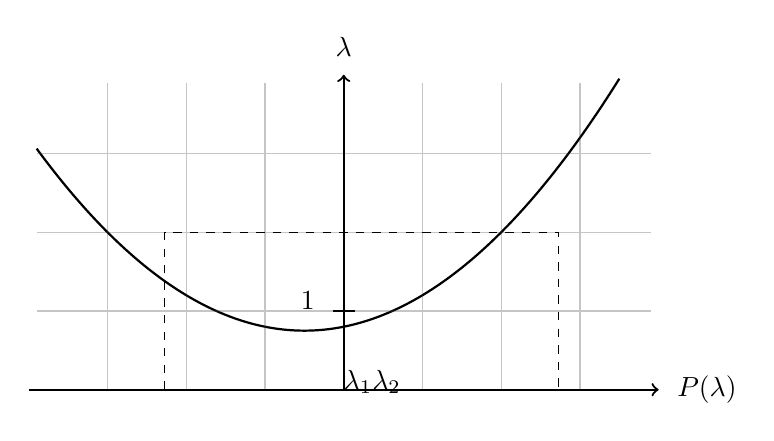
\begin{tikzpicture}
\draw[color=black,thick, variable = \t, samples=200, domain=-3.9:3.5] plot ({\t},{0.2*(\t*\t+\t+4)});
	\draw[step=1, darkgray, opacity=0.3](-3.9,0)grid(3.9,3.9);
	\draw[black,thick,->](-4,0)--(4,0)node[right=3pt]{$P(\lambda)$};
    \draw[black,thick, ->](0,0)--(0,4)node[above=3pt]{$\lambda$};
    \tickx{1}{1}{black};
    \draw(4pt,1)--(-4pt,1)node[left=3pt, yshift=3pt]{\strut 1};
    \tickx{-3}{$\lambda_1$}{black};
    \tickx{2}{$\lambda_2$}{black};
    \tickx{0}{0}{black};
    \draw[dashed](-3,0)--(-3,2)--(2,2)--(2,0);
\end{tikzpicture}
\end{center}
\end{minipage}
\begin{minipage}{0.49\textwidth}
\begin{align*}
&\overbrace{\underbrace{\lambda_2}_{\ge 1}-\underbrace{\lambda_1}_{\le 0}}^{\frac{2}{a}\sqrt{b^2+a(1-c)}}\ge 1\\
\implies& b^2+a(1-c)\ge \left(\frac{a}{2}\right)^2>\frac{\gamma^2}{4}\overset{\eqref{5}}{>}0 \\
\overset{\eqref{5}}{\implies}& x\mapsto \lambda_1(x)\in C^1(\overline{B},\RR)
\end{align*}
\end{minipage}
\end{itemize}
Setze:
\begin{itemize}
\item $x\mapsto g(x):=\lambda_1(x)(f(x)-x)\in C^1(\overline B,\RR^d)$
\item für $t\ge 0$:
\[x\mapsto h_t(x):=x+tg(x)\in C^1(\overline B,\RR^d)\]
\item 
\[V(t):=\int_B\det\underbrace{(Dh_t)(x)}_{\mathds 1+t(Dg)(x)}\dd x\]
\end{itemize}
\textit{Behauptung}: 
\begin{itemize}
\item[(i)]$V(0)=|B|$ (Volumen der Einheitskugel)
\item[(ii)]$V(1)=0$
\item[(iii)]$\hat{g}\colon\begin{array}{clc}
\RR^d&\to&\RR^d\\
x&\mapsto& \left\{\begin{array}{cl}
g(x),&x\in \overline B\\
0,& \text{sonst}
\end{array}\right.
\end{array}$
ist Lipschitz-stetig mit Konstante $L>0$.
\item[(iv)] $h_t\colon \overline B\to\overline B$ ist bijektiv $\forall t\in [0,\frac{1}{2})$.
\end{itemize}
zu (i): klar\\
zu (ii): $\forall x\in\overline{B}$: $|h_1(x)|^2=P(\lambda_1(x)=1$, also $h_1(\overline B)\subseteq \pp B$. Daher ist $(Dh_1)(x)$ nicht invertierbar $\forall x\in B$, denn gäbe es ein $x\in B$ mit $(Dh_1)(x)$ invertierbar würde mit dem Satz über die Umkehrfunktion folgen:
\[\exists \text{Umgebungen (in $\RR^d$) }U\te{von }x\te{und }V\te{von }h_1(x):\;\;h_1\colon U\to V\te{bijektiv \lightning} \]
Also ist $\det(Dh_1)(x)=0$, $\forall x\in B$ und somit $V(1)=0$.\\
zu (iii): \begin{itemize}
\item Da $g\in C^1$ folgt mit dem mehrdimensionalen HDI:
\begin{align*}
&\forall x,y\in B:\;\;g(x)-g(y)=\left(\int_0^1(Dg)(y+s(x-y))\dd s\right)(x-y)\\
\implies& |g(x)-g(y)|\le (\underbrace{\sup_{\xi\in \overline B}\|(Dg)(\xi)\|}_{\underset{\mathclap{\substack{\uparrow\\ g\in C^1(\overline{B},\RR^d)}}}{\le} L<\infty})|x-y|
\end{align*}
\item $x\in \pp B\implies P(0)=|x|^2=1\implies \lambda_1(x)=0\implies g|_{\pp B}=0$
\item Sei $x\in B$, $y\in \RR^d\setminus B$. Dann gilt:\\
\begin{minipage}{0.6\linewidth}
\[|\underbrace{\hat{g}(x)}_{g(x)}-\underbrace{\hat{g}(y)}_{0=g(z)}|=\lim_{B\ni z_n\to z}\underbrace{|g(x)-g(z_n)|}_{\le L|x-z_n|}\le L\underbrace{|x-z|}_{\le |x-y|}\;\;\checkmark\]
\end{minipage}
\begin{minipage}{0.39\linewidth}
\centering
\begin{tikzpicture}
\tkzDefPoint(0,0){O}
\tkzDefPoint(2.5,-1){A}
\tkzDefPoint(0.5,1.5){x}
\tkzDefPoint(3.5,1){y}
\tkzDrawArc[rotate](O,A)(120)
\tkzDrawPoint(x)
\tkzLabelPoint[below=3pt](x){$x$}
\tkzDrawPoint(y)
\tkzLabelPoint[below=3pt](y){$y$}
\tkzDrawLine[dashed](x,y)
\tkzInterLC(x,y)(O,A)
\tkzGetPoints{z}{a}
\tkzDrawPoint(z)
\tkzLabelPoint[above right=3pt](z){$z\in\pp B$}
\path(1,-0.5)node{$B$};
\path(4,-0.5)node{$\RR^d\setminus B$};
\end{tikzpicture}
\end{minipage}
\end{itemize}
zu (iv): Sei $z\in\RR^d$. Betrachte die Fixpunktgleichung $x=z-t\hat{g}(x)$, $x\in\RR^d$. Nach (iii) ist die rechte Seite $\forall t\in [0,\frac{1}{2}[$ eine Kontraktion auf $\RR^d$. Nach dem Banachschen Fixpunktsatz gibt es also genau einen Fixpunkt: 
\[\exists_1 x_z\in\RR^d:\;\;x_z-t\hat{g}(x_z)\]
Somit ist $\hat{h}_t\colon \RR^d\ni x\mapsto x+t\hat{g}(x)$ bijektiv. Da $\hat{h}_t|_{\RR^d\setminus B}=\id$, ist auch $h_t\colon \overline B\to\overline B$ bijektiv.\\
\textit{Finale}:
\begin{itemize}
\item Aus (iv) und der Transformationsformel folgt
\[V(t)=\underbrace{\sgn\left[\det(D_th)(x_0)\right]}_{\text{unabh. von $x_0\in B$}}|\underbrace{h_t(B)}_{\overset{\text{(iv)}}{=}B}|\;\;\;\forall t\in [0,\frac{1}{2}[\tag{$*$}\label{3}\]
\item $D(t):=\det(Dh_t)(x)=\det(\mathds 1+t(Dg)(x))$ ist ein Polynom in $t$, $\forall x\in B$. Daher
\[ \left.\begin{array}{cl}
*&\exists t_0>0\,\forall t\in[0,t_0[:\;D(t)>0\overset{\eqref{3}}{\implies}V(t)=|B|\\
*& V(t)\te{Polynom in }t\te{(per Definition)}
\end{array} \right\}\implies V(t)=\text{const }\forall t\in[0,1]\te{\lightning (i),(ii)}\]\qed
\end{itemize}
\end{Beweis}

Eine weitreichende Verallgemeinerung:

\begin{Satz}{Fixpunktsatz von Schauder}{2.5}
\index{Schauder!Fixpunktsatz von}\index{Fixpunktsatz!Schauder}
Sei $X$ ein normierter Raum, $\emptyset\ne A\subseteq X$ konvex und abgeschlossen. Sei $G\in C(A,A)$ mit $\overline{G(A)}$ kompakt. Dann hat $G$ einen Fixpunkt.
\end{Satz}

Liefert sofort:

\begin{Kor}{}{2.6}
Sei $X$ ein normierter Raum und $\emptyset\ne A\subseteq X$ konvex und kompakt. Dann hat $A$ die Fixpunkteigenschaft.
\end{Kor}

Reduktion von Satz \ref{Satz:2.5} (Schauder) auf endliche Dimensionen (Brouwer) via:
\begin{Lemma}{Projektionslemma von Schauder}{2.7}
\index{Projektionslemma von Schauder}\index{Schauder! Projektionslemma von}
Sei $X$ ein normierter Raum, $\emptyset\ne K\subseteq X$ kompakt. Dann gibt es für alle $\ve>0$ eine endliche Teilmenge $F=\{y_1,\ldots,y_n\}\subseteq K$ und eine stetige Abbildung
\[P\colon K\to \mathrm{convh}(F):=\underbrace{\left\{\sum_{j=1}^nt_jy_j\,:\,\sum_{j=1}^nt_j=1,t_j\ge0\;\forall j=1,\ldots,n\right\}}_{\textbf{konvexe Hülle}}\]
mit $\|P(x)-x\|<\ve\;\;\;\forall x\in K$.
\end{Lemma}

\begin{Beweis}
Sei $\ve>0$. Da $K$ kompakt (und somit totalbeschränkt), $\exists n\in\NN\;\exists y_1,\ldots,y_n\in K$: $K\subseteq \bigcup_{j=1}^nB_{\ve}(y_j)$ ($B_{\ve}(y_j)$ ist der offene $\ve$-Ball um $y_j$ bzgl. $\|\cdot\|$). 
\begin{itemize}
\item Setze für $j\in\{1,\ldots,n\}$:
\[\phi_j\colon \begin{array}{clc}
K&\to &[0,\ve]\\
x&\mapsto& \left\{ \begin{array}{cl}
\ve-\|x-y_j\|,&x\in B_{\ve}(y_j)\\
0,&\text{sonst}
\end{array} \right.
\end{array}\]
$\phi_j$ ist stetig und, da $\phi_j>0$ auf $B_{\ve}(x_j)$:
\[\phi(x):=\sum_{j=1}^n\phi_j(x)>0,\;x\in K\,.\]
\item $P\colon \begin{array}{clc}
K&\to&\mathrm{convh}(\{y_1,\ldots,y_n\})\\
x&\mapsto& \sum_{j=1}^n\frac{\phi_j}{\phi(x)}y_j
\end{array} $ heißt \textbf{Schauder-Projektion} und ist stetig.
\end{itemize}
Für alle $x\in K$ gilt:
\begin{align*}
\|P(x)-x\|
=\left\|\sum_{j=1}^n\frac{\phi_j(x)}{\phi(x)}(y_j-x)\right\|
\le \sum_{j=1}^n\frac{\phi_j}{\phi(x)}\|y_j-x\|
=\sum_{\substack{j\in[n]:\\x\in B_{\ve}(y_j)}}\frac{\phi_j(x)}{\phi(x)}\underbrace{\|y_j-x\|}_{<\ve}
<\ve \sum_{j=1}^n\frac{\phi_j(x)}{\phi(x)}
=\ve
\end{align*}\qed
\end{Beweis}

\begin{Lemma}{}{2.8}
Sei $X$ ein normierter Raum, $\emptyset\ne A\subseteq X$ abgeschlossen und $G\in C(A,A)$ mit $\overline{G(A)}$ kompakt. Für alle $\ve>0$ gebe es ein $\xi\in A$ mit $\|G(\xi)-\xi\|<\ve$. Dann hat $G$ einen Fixpunkt. 
\end{Lemma}

\begin{Beweis}
Nach Voraussetzung gibt es eine Folge $(\xi_n)_n\subseteq A$ mit $G(\xi_n)-\xi_n\xrightarrow{n\to\infty}0$. Da $\overline{G(A)}$ kompakt ist, existiert eine konvergente Teilfolge von $(G(\xi_n))_n$: $\exists (\xi_{n_k})_k\subseteq A\,\exists \eta\in\overline{G(A)}:\;G(\xi_{n_k})\xrightarrow{k\to\infty}\eta$.
\[\implies \xi_{n_k}\xrightarrow{k\to\infty}\eta\overset{A\te{abg.}}{\implies}\eta\in A\implies \eta=\lim_{k\to\infty}G(\xi_{n_k})\overset{G\te{stetig}}{\underset{\eta\in A}{=}}G(\eta)\]\qed
\end{Beweis}

\begin{Beweis}
(von Satz \ref{Satz:2.5}) Sei $G\in C(A,A)$. Nach Voraussetzung ist $K:=\overline{G(A)}$ kompakt. Für $\ve>0$ sei $F:=\{y_1,\ldots,y_n\}$, sodass $K\subseteq \bigcup_{j=1}^nB_{\ve}(y_i)$ und sei $P\colon \mathrm{convh}(F)(\ne\emptyset)$ die Schauder-Projektion. Wegen
\[\mathrm{convh}(\underbrace{F}_{
\mathclap{
\subseteq K=\underbrace{\overline{G(A)}}_{\subseteq A}\;\;\overset{\text{abg.}}{\subseteq}A
}})\subseteq \mathrm{convh}(A)\overset{\mathclap{\substack{A\text{ konvex}\\\downarrow}}}{=}A\]
ist folgende Abbildung wohldefiniert:
\[\tilde{G}:=P\circ G|_{\mathrm{convh}(F)}\colon \mathrm{convh}(F)\to\mathrm{convh}(F)\]
Außerdem ist $\tilde{G}$ stetig. $U:=\RR\text{-}\spann\{y_1,\ldots,y_n\}\supseteq \mathrm{convh}(F)$ ist ein endlich dimensionaler Vektorraum, also: 
\[\exists N\in\NN\,\exists \underbrace{\text{isometrischer Isomorphismus }}_{\text{Homöomorphismus}}\Phi\colon U\to\RR^N\;(N\le n)\]
\[\begin{array}{ll}
\Phi\te{linear}&\implies C:=\Phi(\mathrm{convh}(F))\te{konvex}\\
\Phi\te{isometrisch}&\implies \left.\begin{array}{l}
C\te{abgeschlossen (da $\mathrm{convh}(F)$ abgeschlossen)}\\
C\te{beschränkt (da $\mathrm{convh}(F)$ beschränkt)}
\end{array}\right\}\overset{\substack{\text{endl. dim.}\\\downarrow}}{\implies} C\te{kompakt}
\end{array}\]
Außerdem ist $C\ne \emptyset$.\\
$\implies$ Brouwer (Kor. \ref{Kor:2.4}) und Bem. \ref{Bem:2.3}(a): $\mathrm{convh}(F)$ hat die Fixpunkteigenschaft\\
$\implies$ $\tilde{G}$ hat einen Fixpunkt $\xi\in \mathrm{convh}(F)\subseteq A$.
\[\implies \|\underbrace{\xi}_{\mathclap{\tilde{G}(\xi)=P(G(\xi))}}-G(\xi)\|\overset{\mathclap{\substack{\text{Lemma }\ref{Lemma:2.7}\\ \downarrow}}}{\le}\ve\]
Da $\ve>0$ beliebig, folgt die Behauptung mit Lemma \ref{Lemma:2.8}.\\\qed
\end{Beweis}

\subsection{Existenzssatz von Peano}
Den Existenzsatz von Peano erhält man mittels dem Fixpunktsatz von Schauder. Um die Kompaktheitsvoraussetzung nachzuprüfen, dient der Satz von Arzel\`a-Ascoli.

\begin{Def}{}{2.9}
\index{gleichgradig stetig}
Seien $(X,d)$, $(\tilde{X},\tilde{d})$ metrische Räume und $\FF\subseteq C(X,\tilde{X})$.
\[\FF\textbf{ gleichgradig stetig }:\iff 
\left\{\begin{array}{c}
\forall \ve>0\;\forall x\in X\;\exists \delta>0\; \forall y\in Y\;\forall f\in\FF:\\
d(x,y)<\delta\implies \tilde{d}(f(x),f(y))<\ve
\end{array}  \right.
\]
\end{Def}

\begin{Satz}{Arzel\`a - Ascoli}{2.10}
\index{Arzel\`a-Ascoli}
Sei $(K,d)$ ein kompakter metrischer Raum, $N\in\NN$ und $\FF\subseteq C(K,\KK^N)$ (mit $\sup$-Norm $\|\cdot\|_{\infty}$). Dann gilt:
\[\overline{\FF}\te{kompakt }\iff \FF \te{beschränkt und gleichgradig stetig}\]
\end{Satz}

Wir verwenden im Beweis:

\begin{Lemma}{}{2.11}
\index{totalbeschränkt}
Sei $X$ ein vollständiger metrischer Raum und $A\subseteq X$ totalbeschränkt, das heißt
\[\forall\ve>0\,\exists n\in\NN\,\exists x_1,\ldots,x_n\in A:\; A\subseteq \bigcup_{k=1}^nB_{\ve}(x_k)\,.\]
Dann ist $\overline A$ kompakt.
\end{Lemma}

\begin{Beweis}
Anngenommen $\overline A$ ist nicht kompakt. Dann existiert eine offene Überdeckung $\bigcup_{j\in J}U_j\supseteq \overline A$ ohne endliche Teilüberdeckung. Sei $\ve_1:=2^{-1}$. Dann gibt es nach Voraussetzung $n_1\in\NN$ und $x_1^{(1)},\ldots,x_{n_1}^{(1)}\in A$:
\[\overline{A}\subseteq \overline{\bigcup_{k=1}^{n_1}B_{\ve_1}(x_k^{(1)})}=
\bigcup_{k=1}^{n_1}\overline{B_{\ve_1}(x_k^{(1)})}
\implies \overline A\overset{\substack{\text{sogar }=\\\downarrow}}{\subseteq} \bigcup_{k=1}^{n_1}\left(\overline{B_{\ve_1}(x_k^{(1)})}\cap \overline A\right)
\]
Also $\exists x_{k_1}^{(1)}=:y_1$, sodass $\overline{B_{\ve_1}(y_1)}\cap \overline A$ nicht von endlich vielen der $U_j$ überdeckt wird. Sei $\ve_2:=2^{-2}$. Da $B_{\ve_1}(y_1)\cap A$ totalbeschränkt ist, existiert $n_2\in \NN$ und $x_1^{(2)},\ldots,x_{n_2}^{(2)}\in B_{\ve_2}(y_1)\cap A$:
\[\overline{B_{\ve_1}(y_1)}\cap \overline A\subseteq 
\bigcup_{k=1}^{n_2}\overline{B_{\ve_2}(x_k^{(2)})}
\implies \overline{B_{\ve_1}(y_1)}\cap \overline A\subseteq \bigcup_{k=1}^{n_2}\left(\overline{B_{\ve_2}(x_k^{(2)})}\cap \overline A\right)
\]
Also $\exists x_{k_2}^{(2)}=:y_2$, sodass $\overline{B_{\ve_2}(y_2)}\cap \overline A$ nicht von endlich vielen der $U_j$ überdeckt wird.\\
\ \\
Induktiv: $\exists (y_k)_{k\in\NN}\subseteq A$:
\begin{itemize}
\item[(i)]$\overline{B_{2^{-k}}(y_k)}\cap \overline A$ wird $\forall k\in\NN$ nicht von endlich vielen der $\{U_j\}$ überdeckt.
\item[(ii)]\[d(y_k,y_{k+l})\le \sum_{i=1}^l\underbrace{d(y_{k+i-1},y_{k+i})}_{\underset{\mathclap{\substack{\uparrow\\ \text{für }k\ge 2:\, y_k\in B_{2^{k-1}}(y_{k-1})}}}{\le} 2{-(k+i-1)}}\le 2^{-(k-1)}\;\;\;\forall k,l\in\NN\]
Somit ist $(y_k)_k$ eine Cauchyfolge und da $X$ vollständig ist, existiert ein Grenzwert $y\in \overline{A}$: $y_k\xrightarrow{k\to\infty}y$.
\end{itemize}

\begin{center}
\begin{minipage}{0.49\linewidth}
Nun:
\begin{align*}
&y\in\overline A\implies \exists j_0\in J:\;y\in U_{j_0}\\
\underset{\mathclap{\substack{\uparrow\\U_j\te{offen}}}}{\implies}& \exists \delta >0:\;B_{\delta}(y)\subseteq U_{j_0}
\end{align*}
Wähle $k\in\NN$ so groß, dass
\[\left.
\begin{array}{cl}
\bullet& d(y,y_k)<\dfrac{\delta}{2}\\
\bullet& 2^{-k}<\dfrac{\delta}{2}
\end{array}\right\}
\implies \overline{B_{2^{-k}}(y_k)}\subseteq B_{\delta}(y)\subseteq U_{j_0}
\]
\lightning{} zu (i).
\end{minipage}
\begin{minipage}{0.5\linewidth}
\centering
\begin{tikzpicture}[scale=0.6]
\path[draw,use Hobby shortcut,closed=true]
(-4.5,-2)..(-4.5,2)..(-1,4.4)..(2.5,4.5)..(4.5,2)..(5.5,-1.1)..(3.5,-3.5)..(-1,-4);
\tkzDefPoint(0,0){y}
\tkzDrawPoint(y)\tkzLabelPoint(y){$y$}
\tkzDefPoint(4,0){A}
\tkzDefPoint(2,0){B}
\tkzDefPoint(-0.2,0){C}
\tkzDefPoint(4,4){D}
\tkzDefPoint(4,-3){E}
\tkzDefPoint(-3,1){F}
\tkzDrawCircle[color=black](y,A)
\tkzDrawCircle[dotted, color=black, thick](y,B)
\tkzDefPoint(-1,0){yk}
\tkzDrawPoint(yk)\tkzLabelPoint(yk){$y_k$}
\tkzDrawCircle[color=black](yk,C)
\tkzInterLC(y,D)(y,A)
\tkzGetPoints{a}{b}
\tkzDrawLine[<->, add=-0.1 and -0.1](y,b)
\tkzLabelLine[above=3pt](y,b){$\delta$}
\tkzInterLC(y,E)(y,B)\tkzGetPoints{c}{d}
\tkzDrawLine[<->,add=-0.1 and -0.1](y,d)
\tkzLabelLine[above right](y,d){$\frac{\delta}{2}$}
\tkzInterLC(yk,F)(yk,C)\tkzGetPoints{e}{f}
\tkzDrawLine[<->, add=-0.1 and -0.1](yk,f)
\tkzLabelLine[above, pos=0, yshift=0.5pt](yk,f){\tiny $2^{-k}$}
\path (-3,4.5)node{$U_{j_0}$};
\end{tikzpicture}
\end{minipage}
\end{center}
\qed
\end{Beweis}

\begin{Beweis}
(von Satz \ref{Satz:2.10})\\
\glqq{}$\implies$\grqq{}: Übung\\
\glqq{}$\impliedby$\grqq{}: Zeige, dass $\FF$ total beschränkt, die Behauptung folgt dann mit Lemma \ref{Lemma:2.11}, da $(C(K,\KK^n),\|\cdot\|_{\infty})$ vollständig ist. Sei $\ve>0$. Dann, nach Voraussetzung, 
\[
\forall x\in K\,\exists \delta_x>0\,\forall f\in\FF\,\forall x'\in B_{\delta_x}(x):\;\;|f(x)-f(x')|<\frac{\ve}{4}\tag{$1$}\label{8}
\]
$\{B_{\delta_x}(x)\}_{x\in K}$ ist eine offene Überdeckung von $K$. Weil $K$ kompakt ist, gibt es eine offene Teilüberdeckung:
\[\exists J\in\NN\,\exists x_1,\ldots,x_J\in K:\;\;K\subseteq \bigcup_{j=1}^JB_{\delta_{x_j}}(x_j)\]
Also:
\[|f(x)-f(x_j)|\overset{\eqref{8}}{<}\frac{\ve}{4},\;\forall x\in B_{\delta_{x_j}}(x_j)\;\;\;\forall f\in\FF,\,\forall j=1,\ldots,J\tag{$2$}\label{9}\]
$\FF$ beschränkt $\implies$ $F:=\{f(x_j)\,:\,j=1,\ldots, J,\,f\in\FF\}\subset \KK^N$ beschränkt $\overset{\text{Heine-Borel}}{\underset{\text{in }\KK^N}{\implies}}$ $\overline{F}$ kompakt $\implies$ $\exists L\in\NN\,\exists y_1,\ldots,y_L\in \overline F:\; F\subseteq \bigcup_{l=1}^LB_{\frac{\ve }{4}}(y_l)$\\
\ \\
Für $\vp\colon \{1,\ldots,J\}\to\{1,\ldots,L\}$ sei
\[\FF_{\vp}:=\{f\in\FF\,:\,f(x_j)\in B_{\frac{\ve }{4}}(y_{\vp(j)}),\,\forall j=1,\ldots,J\}\,.\]
Dann ist
\[
\FF=\bigcup_{\vp}\FF_{\vp}\;\;\;\text{(endliche (!) Vereinigung)}\tag{$3$}\label{10}
\]
\textit{Behauptung}: $\diam \FF_{\vp}<\ve$ ($\implies \FF_{\vp}\subseteq \overbrace{B_{\ve}(f_{\vp})}^{\mathclap{\substack{\text{Ball in }C(K,\KK^n)\\\downarrow}}}\overset{\eqref{10}}{\implies} \FF$ total beschränkt)\\
Wahr, da $\forall f,g\in\FF_{\vp},\,\forall x\in K$: Sei $j_0\in \{1,\ldots,J\}$, sodass $x\in B_{\delta_{x_{j_0}}}(x_{j_0})$. Dann:
\[|f(x)-g(x)|\le \underbrace{|f(x)-f(x_{j_0})|}_{\overset{\eqref{9}}{<}\frac{\ve }{4}}
+\underbrace{|f(x_{j_0})-g(x_{j_0})|}_{\underset{\substack{\uparrow\\\text{Def }\FF_{\vp}}}{<}\frac{\ve }{2}}
+\underbrace{|g(x_{j_0})-g(x)|}_{\overset{\eqref{9}}{<}\frac{\ve }{4}}<\ve
\]\qed
\end{Beweis}

\begin{Satz}{Peano}{2.12}
\index{Peano, Existenzsatz von}\index{Existenzsatz!Peano}
Seien $a,b>0$, $x_0\in\RR$ und $y_0\in\RR^d$. Sei $D\supseteq \overline{B_a(x_0)}\times \overline{B_b(y_0)}$ und $f\colon D\to\KK^d$ stetig. Dann gibt es ein $\delta>0$ und eine Lösung $\vp\in C^1([x_0-\delta,x_0+\delta],\KK^d)$ des Anfangswertproblems 
\[\left\{ \begin{array}{l}
y'=f(x,y)\\
(x_0;y_0)
\end{array}\right.\,. \]
\end{Satz}

\begin{Beweis}
Falls $f|_{\overline{B_a(x_0)}\times \overline{B_b(y_0)}}=0$, ist $\vp(x)=y_0$ $\forall x\in \overline{B_a(x_0)}$ eine Lösung. Andernfalls definiere 
\[F:=\sup_{(x,y)\in \overline{B_a(x_0)}\times \overline{B_b(y_0)}} |f(x,y)|\]
 und wähle:
 \begin{center}
\fbox{$\delta:=\min\left(a,\dfrac{b}{F}\right)$}
\end{center}
Sei $I:=[x_0-\delta,x_0+\delta]$ und $A:=\{\vp\in (C(I,\KK^d),\|\cdot\|_{\infty}):\, \|\vp-y_0\|_{\infty}\le b\}$. Dann:
\begin{itemize}
\item[(i)] $A\ne \emptyset$, denn $(x\mapsto y_0)\in A$.
\item[(ii)] $A$ ist abgeschlossen (wegen \glqq$\le$\grqq{}).
\item[(iii)] $A$ ist konvex: Seien $\vp,\psi\in A$ und $\lambda\in[0,1]$. Dann
\[\xi:=\lambda \vp+(1-\lambda)\psi\in C(I,\KK^d)\]
und
\[\|\xi-y_0\|_{\infty}=\|\lambda(\vp-y_0)+(1-\lambda)(\psi-y_0)\|_{\infty}\le \lambda b+(1-\lambda)b=b\,.\]
\end{itemize}
Für $\vp\in A$, $x\in I$ sei: 
\[(G(\vp))(x):=y_0+\int_{x_0}^xf(\underbrace{t,\underbrace{\vp(t)}_{\mathclap{\in \overline{B_b(y_0)}}}}_{\in D})\dd t\;\;\te{(wohldefiniert)}\]
Dann:
\begin{itemize}
\item[(iv)] $G(\vp)\in A$, da:
\begin{itemize}
\item $G(\vp)$ sogar stetig diffbar (HDI, $f$ stetig, $\vp$ stetig)
\item $\|G(\vp)-y_0\|_{\infty}\le \sup_{x\in I}|x-x_0|F\le \delta F\le b$
\end{itemize}
\item[(v)] $G(A)$ ist beschränkt, da (iv) und $A$ beschränkt:
\[\vp\in A\implies \|\vp\|_{\infty}=\|\vp-y_0+y_0\|_{\infty}\le\|\vp-y_0\|_{\infty}+|y_0|\le b+|y_0|<\infty\]
\item[(vi)] $G\in C(A,A)$, da (iv) und: Sei $(\vp_n)_n\subseteq A$, $\vp\in A$ und $\|\vp_n-\vp\|_{\infty}\xrightarrow{n\to\infty}0$. Dann
\[\|G(\vp_n)-G(\vp)\|_{\infty}=\sup_{x\in I}\left|\int_{x_0}^x[f(t,\vp_n(t))-f(t,\vp(t))]\dd t\right|\le \int_I\underbrace{|f(t,\vp_n(t))-f(t,\vp(t))|}_{\le 2F}\dd t\xrightarrow[\text{dom. Kgz.}]{n\to\infty}0\,.\]
(Folgenstetigkeit $\iff$ Stetigkeit, denn $C(A,A)$ ist ein metrischer Raum).
\item[(vii)] $G(A)$ ist gleichgradig (Lipschitz) stetig, da $\forall x_1,x_2\in I$:
\[\sup_{\vp\in A}\left|(G(\vp))(x_1)-(G(\vp))(x_2)\right|
=\sup_{\vp\in A}\left|\int_{x_2}^{x_1}f(t,\vp(t))\dd t\right|\le F|x_1-x_2|
\]
\end{itemize}
(v) und (vii) $\overset{\text{Arz.-Asc}}{\underset{\ref{Satz:2.10}}{\implies}} \overline{G(A)}$ kompakt in $C(I,\KK^d)$ ($I$ kompakt).\\
(i)-(iii) und (vi) $\overset{\text{Fixpkts. Schauder}}{\underset{\ref{Satz:2.5}}{\implies}}\exists \vp\in A:\;\vp=G(\vp)$, das heißt:
\begin{itemize}
\item $\vp\in C(I,\KK^d)$
\item $\{(t,\vp(t))\,:\,t\in I\}\subseteq D$
\item $\vp$ löst die Volterra-Integralgleichung zum AWP ($\implies \vp\in C^1(I,\KK^d)$, vgl. (iv)) $\overset{\text{Satz \ref{Satz:1.11}}}{\implies}$ $\vp$ löst das AWP.\\\qed
\end{itemize}
\end{Beweis}

\begin{Bemerkung}{}{2.13}
\begin{itemize}
\item[(a)] Die Lösung muss nicht unbedingt eindeutig sein (siehe Gegenbeispiel im Tutorium).
\item[(b)] Die Größe des Lösungsintervalls ist optimal für $\delta=\min(a,b/F)$.\\
\ \\
\textit{Beispiel}: $f(x,y)=c\in\RR^d\setminus\{0\}$ für $(x,y)\in\overline{B_a(x_0)}\times \overline{B_b(y_0)}=:D$. Dann hat das AWP
 \[\left\{ \begin{array}{l}
 y'=c\\
 (x_0;y_0)
\end{array}\right.  \]
die eindeutige Lösung $\phi(x)=y_0+c(x-x_0)$ und es gilt
\[(x,\phi(x))\in D\iff |x-x_0|\le a\wedge \underbrace{|\phi(x)-y_0|}_{|c||x-x_0|}\le b
\iff |x-x-0|\le \min\{a,\underbrace{b/|c|}_{b/F}\}\,.
\]
\end{itemize}
\end{Bemerkung}

\begin{Kor}{}{2.14}
Sei $D\subseteq \RR\times \KK^d$ offen, $f\colon D\to\KK^d$ stetig und $K\subset D$ kompakt. Dann $\exists\delta>0$, sodass es $\forall$ Anfangsbedingungen $(x_0,y_0)\in K$ eine Lösung $\vp\in C^1([x_0-\delta,x_0+\delta],\KK^d)$ des AWP $\left\{ \begin{array}{c}
y'=f(x,y)\\
(x_0;y_0)
\end{array}\right. $ gibt.
\end{Kor}

\begin{Beweis}
Verwende die explizite Form von $\delta$ im Beweis des Satzes von Peano und dass $\dist(K,\pp D)>0$ (warum?). Details: Übung!
\end{Beweis}


\subsection{Fortsetzen von Lösungen}
\textit{Ziel}: Vergrößere das (lokale) Lösungsintervall so weit es geht! O.E. sei im Folgenden $\KK=\RR$.

\begin{Satz}{Globaler Existenzsatz}{2.15}
\index{Globaler Existenzsatz}\index{Existenzsatz!Globaler}\index{Kompaktum verlassen}
Sei $D\subseteq \RR\times\RR^d$ offen, $(x_0,y_0)\in D$ und $f\colon D\to\RR^d$ stetig. Dann besitzt das Anfangswertproblem
\[\left\{
\begin{array}{c}
y'=f(x,y)\\
(x_0,y_0)
\end{array}
\right.\tag{$*$}\label{4}\]
mindestens eine Lösung $\vp\colon I\to\KK^d$, deren Graph jedes Kompaktum in beide Richtungen verlässt, das heißt
\[\forall K\subseteq D\te{komapkt mit }(x_0,y_0)\in K\;\exists x_{\pm}\in I\te{mit }x_-<x_0<x_+\te{und }(x_{\pm},\vp(x_{\pm}))\notin K\;.\]
\end{Satz}
Zur Definition \glqq{}Kompaktum in beide Richungen verlassen\grqq{}:
\begin{center}
\begin{tikzpicture}[scale=0.8]
\draw[->](-3,0)--(11,0)node[right=3pt]{$\RR$};
\draw[->](0,-3)--(0,7)node[above=3pt]{$\RR^d$};
\draw[mydarkblue]plot[smooth]coordinates{(0.2,-2)(1,0)(3,3)(4,3.5)(5,4)(7,3)(8.5,5)};
\draw[mydarkred](-1,-1.5)--(-1,3)--(1.5,5)--(8,5)--(8,-1.5)--(-1,-1.5);
\path[draw,use Hobby shortcut,closed=true](-2,0)..(-2.2,3)..(0,4)..(1,6)..(4,5.5)..(9,6)..(8.8,4)..(9,-2)..(7,-1.7)..(-1.5,-1.5);
\path(3,4.5)node[mydarkred]{$K$ kompakt};
\path(7.2,6)node{$D$ offen};
\path(7,2.4)node[mydarkblue]{$\vp(x)$};
\tkzDefPoint(3,3){A}
\tkzDrawPoint[mydarkblue](A)
\tkzDefPoint(0.2,-2){B}
\tkzDrawPoint[mydarkblue](B)
\tkzDefPoint(8.5,5){C}
\tkzDrawPoint[mydarkblue](C)
\tkzDefPoint(0.2,0){xm}
\tkzDefPoint(8.5,0){xp}
\path(3,0)node[below=3pt]{$x_0$};
\path(0,3)node[left=3pt]{$y_0$};
\draw(3,0.1)--(3,-0.1);
\draw(-0.1,3)--(0.1,3);
\draw(0.2,0.1)--(0.2,-0.1);
\draw(8.5,0.1)--(8.5,-0.1);
\tkzDrawLine[add=.0 and .0, dashed, color=mydarkblue](B,xm)
\tkzDrawLine[add=.0 and .0, dashed, color=mydarkblue](C,xp)
\tkzLabelPoint[above right](xm){$x_-$}
\tkzLabelPoint[below=3pt](xp){$x_+$}
\end{tikzpicture}
\end{center}

\begin{Beweis}
\index{kompakt-offene Ausschoepfung@kompakt-offene Ausschöpfung}
\textit{Verlassen nach \glqq{}rechts\grqq}: Sei $K\subseteq D$ kompakt, $(x_0,y_0)\in K$. Sei $(K_n)_{n\in\NN}$ eine \textbf{kompakt-offene}\linebreak
\textbf{Ausschöpfung} von $D$, das heißt $K_n$ kompakt, $K_n\subseteq (K_{n+1})^{\circ}\subseteq K_{n+1}$ $\forall n\in\NN$ und $\bigcup_{n\in\NN}K_n=D$. (z.B. $K_n:=\{x\in D\,|\,\dist(x,\pp D)\ge 1/n\wedge |x|\le n\}$). O.E. sei $(x_0,y_0)\in K_1$ (sonst lasse endlich viele weg). Dann:
\[\exists N\in\NN:\;\;K\subset K_N\tag{$1$}\label{11}\]
Kor. \ref{Kor:2.14} $\implies$ $\forall n\in\NN\,\exists\delta_n>0\,\forall (\hat{x},\hat{y})\in K_n\,\exists \text{Lsg.} \vp\colon [\hat{x},\hat{x}+\delta_n]\to\RR^d$ des AWP $\left\{ \begin{array}{c}
y'=f(x,y)\\
(\hat{x},\hat{y})
\end{array}\right. $\\
Definiere rekursiv:
\begin{itemize}
\item $\phi_{1,1}$ als Lösung von \eqref{4} auf $[x_0,x_0+\delta_1]$
\item $\phi_{1,k+1}$ als Lösung von 
\[\left\{ \begin{array}{l}
y'=f(x,y)\\
x_0+k\delta_1;\phi_{1,k}(x_0+k\delta_1)
\end{array}\right. \]
auf $[x_0+k\delta_1,x_0+(k+1)\delta_1]$, so lange wie $(x_0+k\delta_1,\phi_{1,k}(x_0+k\delta_1))\in K_1$. Dies ist höchstens endlich oft machbar, weil $K_1$ beschränkt. Nun setze die einzelnen Stücke zu einer $C^1$ Funktion zusammen (möglich, weil die Stücke im Funktionswert und der Ableitung an den Bruchstellen übereinstimmen): $\exists \alpha_1>0$ und eine Lösung $\Phi_1$ des AWP ($*$) auf  $[x_0,x_0+\alpha_1]$ mit $\exists n_2\in\NN:\;(x_0+\alpha_1,\Phi_1(x_0+\alpha_1))\in K_{n_2}\setminus K_1$
\item $\phi_{2,1}$ als Lösung des AWP 
\[
\left\{ \begin{array}{l}
y'=f(x,y)\\
(x_0+\alpha_1;\Phi_1(x_0+\alpha_1))
\end{array}\right. \tag{$2$}\label{12}
\]
auf $[x_0+\alpha_1,x_0+\alpha_1+\delta_{n_2}]$.
\item $\phi_{2,k+1}$ als Lösung von... $\overset{\text{wie oben}}{\implies}$ $\exists \alpha_2>0$ und eine Lösung $\Phi_2$ von \eqref{12} auf $[x_0+\alpha_1,x_0+\alpha_1+\alpha_2]$ mit $(x_0+\alpha_1+\alpha_2,\Phi_2(x_0+\alpha_1+\alpha_2))\in K_{n_3}\setminus K_{n_2}$.
\end{itemize}
Per Induktion: $\exists$ strikt isotone Folge $(n_j)_{j\in\NN}$, $n_1=1$, $\forall j\in\NN\,\forall j\in\NN\,\exists \alpha_j>0$ und eine Lösung $\Phi_j$ von \[\left\{  \begin{array}{l}
y'=f(x,y)\\
(x_0+\beta_j^+;\Phi_{j-1}(x_0+\beta_j^+))
\end{array} \right. \,\] mit $\beta_j^+:=\sum_{l=1}^{j-1}\alpha_l$, auf $[x_0+\beta_j^+,x_0+\beta_{j+1}^+]$ mit
$(x_0+\beta_{j+1}^+,\Phi_j(x_0+\beta_{j+1}^+))\in K_{n_{j+1}}\setminus K_{n_j}$. Setze die einzelnen Lösungen zusammen: $\exists$ Lösung $\Phi^+$ von \eqref{4} auf $[x_0,x_0+\overbrace{\lim_{j\to\infty}\beta_j^+}^{=:\beta^+})$ mit
\[\forall n\in\NN\,\exists x_n>x_0:\;\;(x_n,\Phi^+(x_n))\notin K_n\]
$\overset{\eqref{11}}{\implies}$ $\Phi^+$ verlässt jedes Kompaktum $K\subset D$ nach rechts.\\
Skizze der Fortsetzung:
\begin{center}
\begin{tikzpicture}
%%% setting
\draw[->](-0.5,0)--(15,0)node[right=3pt]{$\RR$};
\draw[->](0,-0.5)--(0,7)node[above=3pt]{$\RR^d$};
\draw[mydarkred](0.5,4.5)--(6,4.5)--(6,1.5);
\path(1.5,4.2)node[mydarkred]{$K_1=K_{n_1}$};
\draw[mydarkred](0.5,5.5)--(8.8,5.5)--(8.8,1.5);
\path(1.5,5.2)node[mydarkred]{$K_{n_2}$};
\path[draw,use Hobby shortcut](4.7,6)..(5,6)..(8,6.5)..(8.8,6)..(11,6)..(12,5)..(11,1.5)..(11.2,0.5);
\path(9,6.5)node{$D$};
\path(9.5,5)node[right=8pt]{$\dots$};
%%% graph
\begin{scope}
\clip (0,0)--(0,6.2)--(10.5,6.1)--(11,6)--(11,0)--(0,0);
\draw[yellow!50!orange, line width=2mm,]plot[smooth, tension=1, ]coordinates{(1.5,1.5)(3.5,2)(5.5,2.8)(7.5,3.5)(8.5,4)(9.5,5)(11,6)};
\end{scope}
\begin{scope}
\clip (0,0) rectangle (7.5,3.5);
\draw[green!50!white, line width=1mm]plot[smooth, tension=0.7, ]coordinates{(1.5,1.5)(3.5,2)(5.5,2.8)(7.5,3.5)(8.5,4)(9.5,5)(11,6)};
\draw[myblue]plot[smooth, tension=0.7, ]coordinates{(1.5,1.5)(3.5,2)(5.5,2.8)(7.5,3.5)(8.5,4)(9.5,5)(11,6)};
\end{scope}
\begin{scope}
\clip(7.5,3.5) rectangle (9.5,5);
\draw[magenta, line width=1mm]plot[smooth, tension=0.7,]coordinates{(1.5,1.5)(3.5,2)(5.5,2.8)(7.5,3.5)(8.5,4)(9.5,5)(11,6)};
\draw[cyan,]plot[smooth, tension=0.7,]coordinates{(1.5,1.5)(3.5,2)(5.5,2.8)(7.5,3.5)(8.5,4)(9.5,5)(11,6)};
\end{scope}
\tkzDefPoints{1.5/1.5/x0,3.5/2/A,5.5/2.8/B,7.5/3.5/C,8.5/4/D,9.5/5/E,11/6/F}
\tkzDrawPoints[size=3, color=myblue](x0,A,B,C)
\tkzDrawPoints[size=3, color=cyan](D,E)
\foreach \i in {3.5,5.5}{
\tkzDefPoints{\i/0.1/P,\i/-0.1/Q}
\tkzDrawLine[add=.0 and .0, color=myblue, thick](P,Q)
}
\foreach \i in {7.5}{
\tkzDefPoints{\i/0.1/P,\i/-0.1/Q}
\tkzDrawLine[add=.0 and .0, color=green!50!white!80!black, thick](P,Q)
\tkzLabelPoint[below=3pt](Q){\small $\textcolor{magenta}{\textcolor{green!50!white!80!black}{x_0+}\underbrace{\textcolor{green!50!white!80!black}{\alpha_1}}_{\beta_1}}$}
}
\foreach \i in {8.5}{
\tkzDefPoints{\i/0.1/P,\i/-0.1/Q}
\tkzDrawLine[add=.0 and .0, color=cyan, thick](P,Q)
}
\foreach \i in {9.5}{
\tkzDefPoints{\i/0.1/P,\i/-0.1/Q}
\tkzDrawLine[add=.0 and .0, color=magenta, thick](P,Q)
\tkzLabelPoint[color=magenta, below=3pt](Q){\small $x_0+\underbrace{\alpha_1+\alpha_2}_{\beta_2}$}
}
\draw[thick](-0.1,1.5)node[left=3pt]{$y_0$}--(0.1,1.5);
\draw[thick](1.5,0.1)--(1.5,-0.1)node[below=3pt]{$x_0$};
\foreach \i in {1.5,3.5,5.5}{
\tkzDefPoints{\i/0.4/R, \i+2/0.4/S}
\tkzDrawLine[<->, add=-0.02 and -0.02, color=myblue](R,S)
\tkzLabelLine[color=myblue, above=3pt](R,S){$\delta_1$}
}
\foreach \i in {7.5,8.5}{
\tkzDefPoints{\i/0.4/R, \i+1/0.4/S}
\tkzDrawLine[<->, add=-0.02 and -0.02, color=cyan](R,S)
\tkzLabelLine[color=cyan, above=3pt](R,S){$\delta_2$}
}
\draw[<->, color=green!50!white!80!black](1.5,-2)--(7.5,-2);
\path (4.5,-2)node[above=3pt, color=green!50!white!80!black]{$\alpha_1$};
\draw[<->, color=cyan](7.5,-2)--(9.5,-2);
\path (8.5,-2)node[above=3pt, color=cyan]{$\alpha_2$};
%%% Beschriftung der Teilstücke
\path(2.5,1.75)node[color=myblue, above]{$\phi_{1,1}$};
\path(4.5,2.4)node[color=myblue, above]{$\phi_{1,2}$};
\path(6.5,3.15)node[color=myblue, above]{$\phi_{1,3}$};
\path(8,3.75)node[color=cyan, above]{$\phi_{2,1}$};
\path(9,4.5)node[color=cyan, below right]{$\phi_{2,1}$};
\path(4.5,2.4)node[color=green!50!white!80!black, below=3pt]{$\Phi_1$};
\path(8,3.75)node[color=magenta, below right]{$\Phi_2$};
\path(11,5.5)node[color=yellow!50!orange,]{$\Phi^+$};
\end{tikzpicture}
\end{center}
\textit{Verlassen nach links}: analog $\rightsquigarrow$ Lösung $\Phi^-$ auf $(x_0-\beta^-,x_0]$.\\
Zusammenstückeln bei $x_0$:
\[\Phi\colon \begin{array}{rl}
(x_0-\beta^-,x_0+\beta^+)\to&\RR^d\\
x\mapsto&\left\{ \begin{array}{cl}
\Phi^-(x),&x\le x_0\\
\Phi^+(x),& x>x_0
\end{array}\right.
\end{array}\]\qed\\\
$x_0-\beta^-$ bzw. $x_0+\beta^+$ heißt \textbf{negative} bzw. \textbf{positive Entweichzeit} von $\Phi$.
\index{Entweichzeit}
\end{Beweis}
Die Lösung aus Satz \ref{Satz:2.15} ist im folgenden Sinn maximal:

\begin{Def}{}{2.16}
\index{fortsetzbar}\index{Fortsetzung}\index{maximal}
Sei $\vp\colon I\to\RR^d$ eine Lösung einer DGL oder eines AWPs.
\begin{itemize}
\item $\vp$ heißt \textbf{fortsetzbar}, falls es ein Intervall $J\supsetneq I$ und eine Lösung $\psi\colon J\to\RR^d$ mit $\psi|_I=\vp$ gibt. In diesem Fall heißt $\psi$ \textbf{Fortsetzung} von $\vp$.
\item $\vp$ heißt \textbf{maximal}, falls $\vp$ nicht fortsetzbar ist.
\end{itemize}
\end{Def}

\begin{Satz}{}{2.17}
Sei $D\subseteq \RR\times \RR^d$ offen, $f\colon D\to\RR^d$ stetig und $\vp\colon I\to\RR^d$ eine Lösung des AWP $\left\{ \begin{array}{c}
y'=f(x,y)\\
(x_0;y_0)
\end{array} \right.$. Dann sind folgende Aussagen äquivalent:
\begin{itemize}
\item[(i)] $\vp$ verlässt jedes Kompaktum $(x_0,y_0)\in K\subseteq D$ in beide Richtungen.
\item[(ii)] $\vp$ ist maximal.
\end{itemize}
In diesem Fall gilt: $I\subseteq\RR$ ist offen.
\end{Satz}

\begin{Beweis}
(i)$\implies$(ii): Anngenommen, $\vp$ besitzt eine Fortsetzung nach rechts, das heißt $\exists J\supset I$ und $\xi\in J$ mit $\xi>x\,\forall x\in I$ und eine Lösung $\psi\colon J\to\RR^d$ mit $\psi|_I=\vp$. Dann
\begin{itemize}
\item $(x_0,y_0)\in K:=\{(x,\psi(x))\,|\,x\in[x_0,\xi]\}\subseteq D$ ($K$ kompakt)
\item $(x,\phi(x))\in K,\,\forall x\in I,\,x\ge x_0$, das heißt $\vp$ verlässt $K$ nicht nach rechts \lightning.
\end{itemize}
analog mit Annahme, $\vp$ besäße keine Fortsetzung nach links.\\
(ii)$\implies$(i): siehe Übung\\\qed
\end{Beweis}

Speziell für autonome Differentialgleichungen:
\begin{Kor}{}{2.18}
Sei $D\subseteq \RR^d$ offen, $f\colon D\to\RR^d$ stetig und $\vp\colon I\to D$ eine maximale Lösung des AWP $\left\{ \begin{array}{c}
y'=f(y)\\
(x_0;y_0)
\end{array}\right. $ mit $\overline{\vp(I)}$ kompakt. Dann gilt $I=\RR$.
\end{Kor}

\begin{Beweis}
Angenommen, $I$ sei nach rechts beschränkt (links analog). Dann ist $K:=[x_0,\sup I]\times \overline{\vp(I)}$ kompakt in $\RR\times D=:\tilde{D}$ ( Definitionsbereich für Satz \ref{Satz:2.17}) $\overset{\ref{Satz:2.17}}{\implies}$ $\vp$ verlässt $K$ nach rechts \lightning{} zur Def. von $K$.\\\qed
\end{Beweis}

Unter starken Voraussetzungen gilt mehr:
\begin{Def}{}{2.19}
\index{stetig linear beschränkt}
Sei $J\subseteq\RR$ ein Intervall und $f\colon J\times \RR^d\to\RR^d$ stetig.
\[f\textbf{ stetig linear beschränkt }:\iff \exists \rho,\sigma\colon J\to \RR_+\te{stetig }\forall x\in J,\;y\in\RR^d:\;\;\;|f(x,y)|\le\rho(x)|y|+\sigma(x)\]
\end{Def}

\begin{Satz}{}{2.20}
Sei $J\subseteq \RR$ ein offenes Intervall (möglicherweise unbeschränkt) und $f\colon J\times\RR^d\to\RR^d$ stetig und linear beschränkt. Dann ist jede Lösung der DGL $y'=f(x,y)$ auf ganz $J$ fortsetzbar.
\end{Satz}

Der Beweis benötigt eine Ungleichung von allgemeinem Interesse:

\begin{Satz}{Gronwall-Ungleichung}{2.21}
\index{Gronwall-Ungleichung}
Sei $I\subseteq \RR$ ein Intervall (möglicherweise unbeschränkt), $x_0\in I$ und $u,\alpha,\beta\colon I\to\RR$ messbar, $\beta\ge 0$ und $\beta,\alpha\beta,u\beta\in L^1_{\text{loc}}(I)$. Falls 
\[u(x)\le \alpha(x)+\int_{x_0}^x\beta(x')u(x')\dd x'\;\;\te{für fast alle $x\in I$}\tag{$*$}\label{44}\]
dann gilt
\begin{itemize}
\item[(a)] 
\[u(x)\le \alpha(x)+\int_{x_0}^x\alpha(x')\beta(x')\exp\left(\int_{x'}^x\beta(x'')\dd x''\right)\dd x'\;\;\te{für fast alle $x\in I$}\;.\]
\item[(b)] Falls zusätzlich $\alpha$ isoton (monoton wachsend), so ist
\[u(x)\le \alpha(x)\e^{\int_{x_0}^x\beta(x')\dd x'}\;\;\te{für fast alle $x\in I$}\;.\]
\end{itemize}
\end{Satz}

\begin{Beweis}
\begin{itemize}
\item[(a)]Für $x_0\le x\in I$ setze
\[v(x):=\left(e^{-\int_{x_0}^x\beta(x')\dd x'}\right)\int_{x_0}^x\beta(x')u(x')\dd x'\]
$\overset{\text{abs. stetig}}{\implies}$ für fast alle $x_0\le x\in I$:
\[v'(x)=-\beta(x)e^{-\int\dots}\int\dots+\e^{-\int \dots}\beta(x)u(x)
=\underbrace{\beta(x)}_{\ge 0}\underbrace{\left[u(x)-\int_{x_0}^x\beta(x')u(x')\dd x'\right]}_{\overset{\eqref{44}}{\le} \alpha(x)}\underbrace{e^{-\int_{x_0}^x\beta(x')\dd x'}}_{\ge 0}\]
\begin{align*}
\overset{v(x_0)=0}\implies & v(x)=\int_{x_0}^x v'(x')\dd x'\le\int_{x_0}^x\alpha(x')\beta(x')\e^{-\int_{x_0}^{x'}\beta(x'')\dd x''}\dd x' \tag{$**$} \label{45} \\
\implies& \int_{x_0}^x\beta(x')u(x')\dd x'=\e^{+\int_{x_0}^x\beta(x')\dd x'}v(x)\overset{\eqref{45}}{\le} \int_{x_0}^x\alpha(x')\beta(x')\e^{\int_{x'}^x\beta(x'')\dd x''}\dd x'
\end{align*}
Die Behauptung folgt mit \eqref{44} für fast alle $x_0\le x\in I$. Für $x_0\ge x\in I$ analog.
\item[(b)] (a) und $\alpha$ isoton $\implies$ für fast alle $x_0\le x\in I$:
\[u(x)\le \alpha(x)\bigg{[}1+
\underbrace{\int_{x_0}^x\underbrace{\beta(x')\e^{\int_{x'}^x\beta(x'')\dd x''}}_{\displaystyle-\frac{\dd }{\dd x'}e^{\int_{x'}^x\beta(x'')\dd x''}}
}_{{\displaystyle-e^{\int_{x'}^x\beta(x'')\dd x''}\big{|}_{x'=x_0}^{x'=x}}}
\dd x'\bigg{]}
=\alpha(x)\e^{\int_{x_0}^x\beta(x'')\dd x''}
\]
Für $x_0\ge x\in I$ analog.\\\qed
\end{itemize}
\end{Beweis}

\begin{Beweis}
(von Satz \ref{Satz:2.20}) Sei $\vp\colon J\supseteq I\to\RR^d$ eine maximale Lösung. Zu zeigen:
\[I_{\pm}:=\begin{array}{l}\sup\\\inf\end{array}
I=\begin{array}{l}\sup\\\inf\end{array}J=:J_{\pm}\]
\begin{itemize}
\item[(a)]Angenommen, $I_+<J_+$ (insbesondere $I_+<\infty$). Sei $x_0\in I,\,x_0<I_+$. Volterra Integralgleichung (Satz \ref{Satz:1.11}) und $f$ linear beschränkt $\implies$ $\forall x_0\le x\in I$:
\[|\vp(x)|\le \left|\vp(x_0)+\int_{x_0}^xf(x',\vp(x'))\dd x'\right|
\le |\vp(x_0)|+\int_{x_0}^x\sigma(x')\dd x'+\int_{x_0}^x\rho(x')|\vp(x')|\dd x'
\]
Sei 
\begin{align*}
&S:=\sup_{x'\in[x_0,I_+]}\sigma(x')\overset{\mathclap{\substack{\text{stetig, kompakt}\\\downarrow}}}{<}\infty\\
&R:=\sup_{x'\in[x_0,I_+]}\rho(x')\overset{\mathclap{\substack{\text{stetig, kompakt}\\\downarrow}}}{<}\infty\\
&C:=|\vp(x_0)|+(I_+-x_0)S\;(<\infty)
\end{align*}
$\implies$ $\forall x_0\le x\in I$: $|\vp(x)|\le C+R\int_{x_0}^x|\vp(x')|\dd x'$. Somit folgt mit Satz \ref{Satz:2.21}(b) (alle Funktionen stetig $\implies$ $L^1_{\mathrm{loc}}$):
\[|\vp(x)|\le Ce^{R(x-x_0)}\le C\e^{R(I_+-x_0)}=:\Phi\]
$\implies$ $\vp$ verlässt das Kompaktum $[x_0,I_+]\times \overline{B_{\Phi}(0)}\subseteq J\times \RR^d$ nicht nach rechts \lightning{} Satz \ref{Satz:2.17}, also $I_+=J_+$.
\item[(b)] $I_-=J_-$ analog.
\end{itemize}
\qed
\end{Beweis}

\subsection{Eindeutigkeit von Lösungen}
Eine übliche, hinreichende Bedingung:

\begin{Def}{}{2.22}
\index{lokal Lipschitz}\index{Lipschitz}
Sei $D\subseteq \RR\times\RR^d$ offen, $f\colon D\to\RR^d$. Dann
\[\begin{array}{c}
f\textbf{ lokal Lipschitz}\\
\text{(in der 2. Variablen)}
\end{array} :\iff \left\{\begin{array}{l}
\forall (x,y)\in D\,\exists\te{Umgebung $U\subseteq D$ von }(x,y)\;\exists L>0\\
\forall (x',y_1),(x',y_2)\in U:\;\;|f(x',y_1)-f(x',y_2)|\le L|y_1-y_2|
\end{array}\right. \]
\end{Def}

\begin{Satz}{Globale Existenz und Eindeutigkeit}{2.23}
Sei $D\subseteq \RR\times\RR^d$ offen, $(x_0,y_0)\in D$, $f\colon D\to\RR^d$ stetig und lokal Lipschitz. Dann existiert genau eine Lösung $\vp$ des AWP $\left\{\begin{array}{c}
y'=f(x,y)\\
(x_0;y_0)
\end{array}\right.$ deren Graph jedes Kompaktum $(x_0,y_0)\in K\subseteq D$ in beide Richtungen verlässt.
\end{Satz}

\begin{Bemerkung}{}{2.24}
Existenz folgt bereits aus Satz \ref{Satz:2.15}, kann aber auch ohne diesen mittels Banachschem Fixpunktsatz gefolgert werden: Satz von Picard-Lidelöf
\end{Bemerkung}

\begin{Beweis}
Nur Eindeutigkeit ist zu zeigen.
\textit{Annahme}: $\exists$ Intervall $I\ni x_0$ und Lösungen $\vp_1\ne \vp_2$ des AWPs auf $I$. O.E. sei $\vp_1(x)\ne\vp_2(x)$ für ein $x_0<x\in I$ (Fall $x_0>x\in I$ analog). Sei 
\needspace{3cm}
\[\hat{x}_0:=\inf\{\tilde{x}>x_0\,:\,\vp_1(\tilde{x})\ne\vp_2(\tilde{x})\}\in[x_0,x{[}_{\mathord{\tikz[baseline=(B.base), inner sep = 0pt]{\node (B){};}}}\implies 
\vp_1(\hat{x}_0)\,{=}_{\mathord{\tikz[baseline=(C.base), inner sep = 0pt]{\node (C){};}}}\vp_2(\hat{x}_0)=:\hat{y}_0\]
\[\hspace{4cm}\overbrace{\vp_j\te{stetig}}^{\mathord{\tikz[baseline=(D.base), inner sep = 0pt]{\node (D){};}}}\]

\begin{tikzpicture}[overlay]
    \draw [->] (D) to[out=40,in=270]	([shift={(-4pt,-1pt)}]C.center);
    \draw [->] (D) to[out=140,in=270]	(B.south);
\end{tikzpicture}
\vspace{-0.2cm}\\
Nach Voraussetzung $\exists$ Umgebung $U\subseteq D$ von $(\hat{x}_0,\hat{y}_0)$, worauf $f$ Lipschitz. $U$ offen $\implies$ $\exists$ offenes Intervall $J\subseteq \RR$, $x_0\in J$, $\exists \ve>0$: $J\times B_{\ve}(\hat{y}_0)\subseteq U$.\\
Nun wähle $\hat{x}\in ]\hat{x}_0,x]$, sodass
\begin{itemize}
\item $\hat{x}\in J$
\item $\vp_1(\hat{x})\ne\vp_2(\hat{x})$ (möglich per Def. von $\hat{x}_0$)
\item $\vp_j(x')\in B_{\ve}(\hat{y}_0)$, $\forall x'\in[\hat{x}_0,\hat{x}]$, $j=1,2$ (möglich, da $\vp_j$ stetig)
\end{itemize}
\begin{align*}
\overset{\text{Volterra (\ref{Satz:1.11})}}{\implies}& 
|\vp_1(\hat{x})-\vp_2(\hat{x})|
=\bigg{|}\underbrace{\vp_1(\hat{x}_0)-\vp_2(\hat{x}_0)}_{0}+\int_{\hat{x}_0}^{\hat{x}}[f(x',\vp_1(x'))-f(x',\vp_2(x'))]\dd x'\bigg{|}\\
&\le \int_{\hat{x}_0}^{\hat{x}}
\underbrace{f(x',\vp_1(x'))-f(x',\vp_2(x'))}_{
\overset{\substack{\text{lok. Lip.}\\\downarrow}}{\le}
\underbrace{L_{(\hat{x}_0,\hat{y}_0)}}_{=:L}
|\vp_1(x')-\vp_2(x')|,\;\forall x'\in[\hat{x}_0,\hat{x}]}\dd x'\\
\overset{\text{Gronwall-Ungl. (\ref{Satz:2.21})}}{\implies}& |\vp_1(x')-\vp_2(x')|\le \underbrace{0}_{\mathclap{\substack{\uparrow\\ \alpha(t)\te{in Satz \ref{Satz:2.21}}}}}\cdot \e^{L(\hat{x}-\hat{x}_0)}=0\;\te{\lightning}
\end{align*}
\qed
\end{Beweis}

%%%%% Vorlesung 9
\section{Lineare Differentialgleichungen}
Wichtig, denn es gibt eine \glqq vollständige\grqq{} Lösungstheorie.

\begin{Def}{}{3.1}
\index{System linearer Differentialgleichungen}\index{Differentialgleichung!linear}\index{Inhomogenität}\index{Differentialgleichung!homogen}\index{Differentialgleichung!inhomogen}
Sei $I\subseteq \RR$ ein Intervall (möglicherweise unbeschränkt), sei $d\in\NN$ und seien $A\colon I\to\KK^{d\times d}$, $b\colon I\to \KK^d$. Ein \textbf{System linearer Differentialgleichungen} erster Ordnung ist ein System der Form
\[
y'=A(x)y+\underbrace{b(x)}_{\mathclap{\substack{\uparrow\\\text{Inhomogenität}}}}\;.\tag{$\square$}\label{13}\]
Ein System linearer DGL heißt \textbf{homogen}, gdw $b=0$. Man kann ein $d$-dimensionales System auch gemäß Satz \ref{Satz:1.4} in eine lineare DGL $d$-ter Ordnung umwandeln.
\end{Def}

\begin{Beispiel}{Harmonischer Oszillator in einer Raumdimension (Beispiel \ref{Beispiel:1.6})}{3.2}
\index{harmonischer Oszillator}
\[\frac{\dd}{\dd t}\vv{x\\p}=\vv{0&1/m\\-\kappa&0}\vv{x\\p}\]
\end{Beispiel}

\begin{Satz}{Superpositionsprinzip}{3.3}
\index{Superpositionsprinzip}
Seien $\vp_1,\vp_2\colon I\to\KK^d$ Lösungen von \eqref{13} und seien $c_1,c_2\in\KK$. Dann erhalten wir für
\[\psi\colon I\to\KK^d,\;\;\psi=c_1\vp_1+c_2\vp_2\;,\]
dass
\[\psi'(x)=c_1\vp_1'(x)+c_2\vp_2'(x)=c_1A(x)\vp_1+c_1b(x)+c_2A(x)\vp_2+c_2b(x)=A(x)\psi(x)+(c_1+c_2)b(x)\,.\]
Das heißt, $\psi$ löst
\[y'=A(x)+(c_1+c_2)b(x)\,.\tag{$*$}\]
Insbesondere gilt
\begin{itemize}
    \item[(a)] \[\LL_{\text{hom}}:=\{\vp\colon I\to\KK^d\,:\,\te{$\vp$ löst homogene DGL}\}\] 
    ist ein Vektorraum.
    \item[(b)] \[\{\vp\colon I\to\KK^d\,:\,\te{$\vp$ löst inhomogene DGL}\}=\phi_{\text{part}}+\LL_{\text{hom}}\;,\]
    wobei $\vp_{\text{part}}$ irgendeine Lösung der inhomogenen DGL ist.
\end{itemize}
\end{Satz}

\begin{Beweis}
\begin{itemize}
    \item[(a)] Folgt aus Rechnung im Satz mit $b=0$.
    \item[(b)] \glqq $\supseteq$\grqq: $(\vp_{\mathrm{part}}+\vp_{\mathrm{hom}})'(x)=A(x)\vp_{\mathrm{part}}(x)+b+A(x)\vp_{\mathrm{hom}}(x)$\\
    \glqq $\subseteq$\grqq: Sei $\vp$ Lösung der inhomogenen Gleichung, dann löst $\vp-\vp_{\mathrm{part}}$ die homogene DGL.\\\qed
\end{itemize}
\end{Beweis}

\begin{Satz}{Existenz und Eindeutigkeit maximaler Lösungen}{3.4}
Sei $I\subseteq \RR$ ein offenes Intervall (möglicherweise unbeschränkt) und $A\colon I\to\KK^{d\times d}$, $b\colon I\to\KK^d$ stetig. Weiter seien $x_0\in I$ und $y_0\in\KK^d$. Dann existiert genau eine Lösung $\vp\in C^1(I,\KK^d)$ des AWPs \[\left\{\begin{array}{l}
     y'=A(x)y+b(x)\\
     (x_0,y_0)
\end{array}\right.\;,\] die jedes Kompaktum $K\subset I\times \KK^d$, $(x_0,y_0)\in K$ beidseitig verlässt.
\end{Satz}

\begin{Beweis}
Aus Satz \ref{Satz:2.23}, lokale Lipschitzstetigkeit aus Linearität und Stetigkeit von $A$.
\end{Beweis}

\begin{Kor}{}{3.5}
Es gelten die Voraussetzungen von Satz \ref{Satz:3.4}. Sei $d\ge 2$ und $n\in\{2,\ldots,d\}$. Seien $\vp_1,\ldots,\vp_n$ Lösungen der homogenen DGL \eqref{13} und sei $x_0\in I$. Dann sind folgende Aussagen äquivalent:
\begin{itemize}
    \item[(i)] $\exists x_0\in I:\;\; \vp_1(x_0),\ldots,\vp_n(x_0)$ sind linear abhängig.
    \item[(ii)] $\forall x\in I:\;\;  \vp_1(x),\ldots,\vp_n(x)$ sind linear abhängig. 
\end{itemize}
\end{Kor}

\begin{Beweis}
Nur (i) $\implies$ (ii) ist nichttrivial. N.V. $\exists c_1,\ldots,c_n\in\KK$: $\sum_{\nu=1}^nc_{\nu}\vp_{\nu}(x_0)=0$. Sei
\[\psi:=\sum_{\nu=1}^nc_{\nu}\vp_{\nu}\in C^1(I,\KK^d)\overset{\text{Satz }\ref{Satz:3.3}}{\implies} \psi\te{löst das AWP }\left\{ \begin{array}{c}
y'=Ay\\
(x_0,0)
\end{array}\right. \]
Dieses hat $\vp(x)\equiv0$ als Lösung. Nach Satz \ref{Satz:3.4} ist diese Lösung eindeutig, also $\psi(x)=0$, $\forall x\in I$.\\\qed
\end{Beweis}

\begin{Kor}{}{3.6}
In der Situation von Kor. \ref{Kor:3.5} gilt
\[\dim \LL_{\text{hom}}=d\;.\]
\end{Kor}

\begin{Def}{}{3.7}
\index{Fundamentalsystem}\index{Fundamentalmatrix}
Seien $\vp_1,\ldots,\vp_d\in C^1(I,\KK^d)$ linear unabhängige Lösungen der homogenen DGL $y'=A(x)y$(\textbf{Fundamentalsystem}). 
\[\Psi\colon \begin{array}{clc}
I&\to&\KK^{d\times d}\\
x&\mapsto&\vv{\vp_1(x)&\cdots&\vp_d(x)}
\end{array}
\]
heißt \textbf{Fundamentalmatrix}.
\end{Def}

\begin{Bemerkung}{}{3.8}
\begin{itemize}
    \item[(a)] $\Psi\in C^1(I,\KK^{d\times d})$ mit $\Psi'(x)=\vv{A(x)\phi_1(x)&\cdots&A(x)\vp_d(x)}=A(x)\Psi(x)$, $\forall x\in I$
    \item[(b)] Sei $x_0\in I$ und $y_0\in\KK^d$. Dann löst 
    $I\ni x\mapsto \Psi(x)\Psi(x_0)^{-1}y_0$ das AWP
    $\left\{\begin{array}{c}
         y'=A(x)y\\ (x_0,y_0)
    \end{array}\right.$
    und $I\ni x\mapsto \Psi(x)\Psi(x_0)^{-1}=:\Phi_{x,x_0}$ das matrixwertige AWP
    $\left\{\begin{array}{c}
         M'=A(x)M\\
         (x_0,\mathds1)
    \end{array}\right.$.
\end{itemize}
\end{Bemerkung}

Die Fundamentalmatrix ist nützlich für:

\begin{Satz}{Variation der Konstanten}{3.9}
\index{Variation der Konstanten}
Sei $I\subseteq \RR$ ein offenes Intervall (möglicherweise unbeschränkt), $A\colon I\to \KK^{d\times d}$, $b\colon I\to\KK^d$ stetig. Sei $\Psi$ eine Fundamentalmatrix zur homogenen DGL $y'=A(x)y$. Sei $x_0\in I$, $y_0\in \KK^d$. Dann ist
\[\vp\colon\begin{array}{clc}
 I&\to&\KK^d\\
x&\mapsto& \Psi(x)\left[\Psi(x_0)^{-1}y_0+\int_{x_0}^x\Psi(x')^{-1}b(x')\dd x'\right]
\end{array}\]
die eindeutige Lösung des inhomogenen AWP
\[\left\{\begin{array}{c}
         y'=A(x)y+b(x)\\
         (x_0,y_0)
    \end{array}\right.\;.\]
\end{Satz}

\begin{Beweis}
$\vp$ ist wohldefiniert, da $\Psi$ stetig und invertierbar auf $I$ (zudem $C^1$) $\implies$ $\Psi^{-1}$ stetig $\implies \int \dd x'$ wohldefiniert und $C^1$ in $x$ $\implies\vp\in C^1(I,\KK^d)$. Weiterhin
\begin{itemize}
\item $\vp(x_0)=\Psi(x_0)[\Psi(x_0)^{-1}y_0+0]=y_0$
\item $\vp'(x)=A(x)\vp(x)+\underbrace{\Psi(x)\Psi(x)^{-1}}_{\mathds 1}b(x)$, $\forall x\in I$
\end{itemize}
\qed
\end{Beweis}

Damit genügt es von nun an, homogene lineare DGL'en zu betrachten.

\begin{Def}{}{3.10}
\index{zeitgeordnete e-Funktion}
\begin{itemize}
    \item[(a)] Sei $B\in\KK^{d\times d}$. Setze $\e^B:=\exp(B):=\sum_{n=0}^{\infty}\frac{1}{n!}B^n$ (\textbf{e hoch Matrix})
    \item[(b)] Sei $A\in C(I,\KK^{d\times d})$, seien $x_0,x\in I$. Setze
    \[\overleftarrow{\exp}\left(\int_{x_0}^xA(x')\dd x'\right):=\mathds1 +\sum_{n=1}^{\infty}\int_{x_0}^x\int_{x_0}^{x_n}\cdots\int_{x_0}^{x_2}A(x_n)\cdots A(x_1)\dd x_1\ldots\dd x_n\]
    oder Physiker-Notation:
    \[\overleftarrow{\exp}\left(\int_{x_0}^xA(x')\dd x'\right)=\mathds 1+\sum_{n=1}^{\infty}\int_{x_0}^x\dd x_n\int_{x_0}^{x_n}\dd x_{n-1}\cdots\int_{x_0}^{x_2}\dd x_1 A(x_n)\cdots A(x_1)\]
    (\textbf{zeitgeordnete e-Funktion})
\end{itemize}
\end{Def}

\begin{Lemma}{}{3.11}
\begin{itemize}
    \item[(a)] Die Reihen in \ref{Def:3.10} (a) und (b) konvergieren in der Abbildungsnorm $\|\cdot\|$, in (b) sogar gleichmäßig in $x\in I$ auf Kompakta .
    \item[(b)] Falls $[A(x),A(x')]=0$ für alle $x,x'\in I$:
    \[\overleftarrow{\exp}\left(\int_{x_0}^xA(x')\dd x'\right)=\exp\left(\int_{x_0}^xA(x')\dd x'\right)\]
\end{itemize}
\end{Lemma}
Zum Beweis von Lemma \ref{Lemma:3.11}(a) das allgemeine Resultat:

\begin{Lemma}{}{3.12}
Sei $X$ ein Banach-Raum und $(x_n)_n\subseteq X$. Dann gilt
\[\sum_{n\in\NN}\|x_n\|<\infty\implies \sum_{n\in\NN}x_n\te{ist in $X$ konvergente Reihe}\]
\end{Lemma}

\begin{Beweis}
Zeige $(y_N)_{N\in\NN}$, $y_N:=\sum_{n=1}^Nx_n$, ist eine Cauchy-Folge in $X$. Seien $N,M\in \NN$, $N\ge M$. Dann
\[\|\underbrace{y_N-y_M}_{\displaystyle\sum_{n=M+1}^Nx_n}\|\le \sum_{n=M+1}^N\|x_n\|=\xi_N-\xi_M=|\xi_N-\xi_M|\]
mit $\xi_K:=\sum_{n=1}^K\|x_n\|$, $K\in\{M,N\}$; nach Voraussetzung $(\xi_N)_N$ Cauchy in $\RR$.\\\qed
\end{Beweis}

\begin{Beweis}
(von Lemma \ref{Lemma:3.11}) Wir zeigen zunächst: Unter den Voraussetzungen von (b) gilt $\forall n\in\NN$:
\[\int_{x_0}^x\dd x_n\int_{x_0}^{x_n}\dd x_{n-1}\dots\int_{x_0}^{x_2}\dd x_1A(x_1)\cdot \dots\cdot A(x_n)=\frac{1}{n!}\left(\int_{x_0}^xA(x')\dd x'\right)^n\tag{$*$}\label{46}\]
Beweis per Induktion: $n=1$ klar; $n-1\rightsquigarrow n$:
\[\int_{x_0}^x\dd x_n\underbrace{\int_{x_0}^{x_n}\dd x_{n-1}\dots\int_{x_0}^{x_2}\dd x_1A(x_1)\cdot \dots\cdot A(x_n)}_{\mathclap{\displaystyle
\overset{\substack{\text{I.V.}\\\downarrow}}{=}\frac{1}{(n-1)!}
\underbrace{\displaystyle A(x_n)\left(\int_{x_0}^{x_n}A(x')\dd x'\right)^{n-1}}_{\mathclap{\displaystyle\frac{1}{n}\frac{\dd }{\dd x_n}\left(\int_{x_0}^{x_n}A(x')\dd x'\right)^n\te{(Vertauschbarkeit geht ein)}}}
}}
=\frac{1}{n!}\left(\int_{x_0}^{x_n}A(x')\dd x'\right)\bigg{|}_{x_n=x_0}^{x_n=x}\overset{\substack{\text{Konv.}\\\text{vorausgesetzt}}}{\implies}\text{(b)}\]
Zu (a): Sei $a:=\sup_{x'\in K}\|A(x)\|$, $K\supseteq [\min(x,x_0),\max(x,x_0)]$ kompakt, $K\subseteq I$. Dann
\begin{align*}
&\left\|\int_{x_0}^x\dd x_n\dots\int_{x_0}^{x_2}\dd x_1A(x_n)\cdot\dots\cdot A(x_2) \right\|\le 
\bigg|\int_{x_0}^x\dd x_n\dots\int_{x_0}^{x_2}\dd x_1\underbrace{\|A(x_n)\cdot\dots\cdot A(x_2)\|}_{\displaystyle\le \prod_{j=1}^n\|A(x_j)\|}\bigg|\\
&\le a^n\bigg|\underbrace{\int_{x_0}^x\dd x_n\dots\int_{x_0}^{x_2}\dd x_1}_{\displaystyle\underset{\substack{\uparrow\\ \eqref{46}\te{mit}\\ A\equiv \mathds 1}}{=}\frac{1}{n!}\left(\int_{x_0}^x\dd x'\right)^n}\bigg|
=\frac{a^n|x-x_0|^n}{n!}
\le \frac{a^n(\diam(K))^n}{n!}
\end{align*}
Somit folgt Konvergenz in Def. \ref{Def:3.10}(b) aus Lemma \ref{Lemma:3.12}, da die Exponentialreihe konvergent, glm. in $x\in K$. Die Reihe in in Def. \ref{Def:3.10}(a) ist der Spezialfall $x_0=0$, $x=1$ und $A(x')=B$, $\forall x'\in I$, siehe \eqref{46}.\\\qed
\end{Beweis}

\begin{Satz}{}{3.13}
Sei $I$ offen, $A\colon I\to\KK^{d\times d}$ stetig, $x_0\in I$, $y_0\in\KK^d$. Dann ist
\[\vp\colon \begin{array}{clc}
I&\to&\KK^d\\
x&\mapsto& \overleftarrow{\exp}\left(\int_{x_0}^xA(x')\dd x'\right)y_0
\end{array}
\]
die eindeutige maximale Lösung des homogenen linearen AWP $\left\{ \begin{array}{c}
y'=A(x)y\\
(x_0;y_0)
\end{array}\right. $.
\end{Satz}

\begin{Beweis}
Volterra-Integralgleichung (Satz \ref{Satz:1.11}) nachrechnen:
\[\text{Lemma }\ref{Lemma:3.11}\implies \vp(x)=y_0+\sum_{n=1}^{\infty}\underbrace{\int_{x_0}^x\dd x_n\int_{x_0}^{x_n}\dd x_{n-1}\cdots\int_{x_0}^{x_2}\dd x_1 (A(x_n)\cdots A(x_1)y_0)}_{=:v_n(x)}\]
konvergiert bzgl. $|\cdot|$ in $\KK^d$ gleichmäßig auf Kompakta in $I$.
\begin{align*}
&|v_n(x)|\le\left|\int_{x_0}^x\dd x_n\int_{x_0}^{x_n}\dd x_{n-1}\cdots\int_{x_0}^{x_2}\dd x_1\prod_{j=1}^n\|A(x_n)\||y_0|\right|
\le \big(\underbrace{\sup_{x'\in K}\|A(x')\|}_{\underset{\mathclap{\substack{\uparrow\\ K\subset I\te{kompakt, }[\min(x,x_0),\max(x,x_0)]\subset K}}}{=}:a}\big)^n\frac{|x-x_0|^n}{n!}|y_0|\\
\overset{\forall j\in\{1,\ldots,d\}}{\underset{\forall x'\in I}{\implies}}&\left|\sum_{n=1}^N(A(x')v_n(x'))_j\right|\le a\sum_{n=1}^Na^n\frac{|x'-x_0|^n}{n!}|y_0|\le a|y_0|e^{a|x'-x_0|}
\end{align*}
ist eine von $N$ unabhängige über $x'\in K$ integrierbare Majorante. Also folgt mit dominierter Konvergenz:
\begin{align*}
&y_0+\int_{x_0}^xA(x')\vp(x')\dd x'\\
=& y_0+\int_{x_0}^xA(x')\dd x'y_0+\underbrace{\sum_{n=1}^{\infty}\int_{x_0}^x\dd x'A(x')\int_{x_0}^{x'}\dd x_n\dots\int_{x_0}^{x_2}\dd x_1 A(x_n)\cdot\dots\cdot A(x_1)y_0}_{\displaystyle\sum_{n=2}^{\infty}\int_{x_0}^{x'}\dd x_n\dots\int_{x_0}^{x_2}\dd x_1 A(x_n)\cdot\dots\cdot A(x_1)y_0}=\vp(x)
\end{align*}
$\overset{\text{Satz }\ref{Satz:1.11}}{\implies}$ $\vp$ löst das AWP, da $\vp$ stetig in $x$ (Übung). Eindeutigkeit folgt aus Satz \ref{Satz:3.4}.\\\qed
\end{Beweis}

\begin{Bemerkung}{}{3.14}
Im Allgemeinen lässt sich $\overleftarrow{\exp}\left(\int_{x_0}^xA(x')\dd x'\right)$ nicht explizit bestimmen, aber im autonomen Spezialfall ist folgendes Korollar nützlich:
\end{Bemerkung}

\begin{Kor}{}{3.15}
Sei $A\in\KK^{d\times d}$, $x_0\in\RR$, $y_0\in\KK^d$. Dann ist
\[\vp\colon \begin{array}{clc}
\RR&\to&\KK^d\\
x&\mapsto&\e^{A(x-x_0)}y_0
\end{array}\]
die eindeutige maximale Lösung des Anfangswertproblems $\left\{\begin{array}{c}
y'=Ay\\(x_0;y_0)
\end{array}\right. $.
\end{Kor}

Die Berechnung des Matrix-Exponentials erfolgt mittels Jordan-Normalform oder dem Putzer-Algorithmus (später), zuvor jedoch:

\begin{Kor}{}{3.16}
Mit der Notation aus Bemerkung \ref{Bem:3.8}(b) folgt für alle $x\in I$:
\[\Phi_{x,x_0}=\Psi(x)\Psi(x_0)^{-1}=\overleftarrow{\exp}\left(\int_{x_0}^xA(x')\dd x'\right)\;,\]
wobei $\Psi=\vv{\vp_1&\dots&\vp_d}$ und $\{\vp_j\}_{j=1,\ldots,d}$ beliebige linear unabhängige Lösungen von $y'=A(x)y$ sind.
\end{Kor}

\begin{Satz}{Formel von Liouville}{3.17}
\index{Formel von Liouville}\index{Liouville!Formel von}\index{Wronski-Determinante}
Sei $A\in C(I,\RR^{d\times d})$ und $x_0\in I$. Dann gilt für die \textbf{Wronski-Determinante} $W:=\det \Psi\in C^1(I,\RR)$:
\begin{center}
\fbox{$\displaystyle W(x)=W(x_0)\exp\left(\int_{x_0}^x\tr A(x')\dd x'\right),\;\;\;\forall x\in I$}\end{center}
\end{Satz}

%%%% Vorlesung 11 
\begin{Beweis}
Sei $x\in I$. Zu zeigen:
\[\log\det\Phi_{x,x_0}=\int_{x_0}^x\tr A(x')\dd x'\]
Sei $0\ne h\in\RR$ mit $x+h\in I$. Differenzenquotient Zähler:
\begin{align*}
&\log\det\Phi_{x+h,x_0}-\log\det\Phi_{x,x_0}=\log\det(\overbrace{\Phi_{x+h,x_0}\Phi_{x,x_0}^{-1}}^{\mathclap{=\Psi(x+h)\Psi(x)=:\Phi_{x+h,x}}})\\
=&\log \det \underbrace{\overleftarrow{\exp}\left(\int_{x}^{x+h}A(x')\dd x'\right)}_{\mathclap{\substack{=\mathds1+\int_x^{x+h}A(x')\dd x'+\OO(h^2)\\\text{(Details: Übung!)}}}}
=\log\left(1+\int_x^{x+h}A(x')\dd x'+\OO(h^2)\right)\\
\iff&\frac{\log\det\Phi_{x+h,x_0}-\log\det\Phi_{x,x_0}}{h}\xrightarrow{h\to0}\tr A(x)\;,
\end{align*}
wobei wir im vorletzten Schritt den Mittelwertsatz der Integralrechnung und die Stetigkeit des Integranten verwendet haben.
Weil $\Phi_{x_0,x_0}=\mathds1$, folgt
\[\log\det\Phi_{x,x_0}=\int_{x_0}^x\tr A(x')\dd x'\]
\qed
\end{Beweis}

\begin{Satz}{Jordan Normalform}{3.18}
\index{Jordan Normalform}
Sei $A\in\CC^{d\times d}$ und $\{\lambda_j\}_j$ die Menge der Eigenwerte gezählt mit geometrischer Vielfachheit. Dann gibt es ein $T\in \Gl_{\CC}(d)$ und für alle $j$ ein $m_j\in\NN$ mit $\sum_jm_j=d$:
\[A=T\bigoplus_j(\lambda\overbrace{\mathds1_{m_j}}^{\ms{m_j\times m_j}\te{Einheitsmatrix}\\ \downarrow}+J_{m_j})T^{-1}\;.\]
\begin{itemize}
\item  $J_1=:0\in \CC^{1\times 1}$
\item Jordan-Block: $J_{\mu}:=\vv{0&1&\dots&0\\\vdots&\ddots&\ddots&\vdots\\
0&0&\ddots&1\\
0&0&0&0
}$ ($\mu\times\mu$-Matrix) für $\mu\in\NN\setminus\{1\}$
\end{itemize}
\end{Satz}

\begin{Beweis}
Lineare Algebra
\end{Beweis}

\begin{Bemerkung}{}{3.18}
\index{Hauptvektor}
\begin{itemize}
\item Für Matrizen: $A\oplus B=\vv{A&0\\0&B}$
\item geometrische Vielfachheit von Eigenwert $\lambda$: $\dim \ker(A-\lambda\mathds1)=:\mathrm{geo}(\lambda)$
\item $T=\vv{T_1&T_2&\dots}$
\begin{itemize}
\item[(i)]Falls $m_j=1$, dann folgt  $T_j=v_j$ mit $v_j$ Eigenvektor zu $\lambda_j$.
\item[(ii)] Falls $m_j>1$, so ist $T_j=\vv{v_j^0&v_j^1&\dots&v_j^{m_j-1}}$, mit den Hauptvektoren: 
\[(A-\lambda_j\mathds1)v_j^k=v_j^{k-1}\]
Gut zur Bestimmung von Hauptvektoren aus Eigenvektor, falls die geometrische Vielfachheit gleich eins ist.
\end{itemize}
\item Für alle $j$ gilt: $m_j\le\text{alg}(\lambda_j)-\text{geo}(\lambda_j)+1$ mit Gleichheit falls $\text{geo}(\lambda_j)=1$.
\end{itemize}
\end{Bemerkung}

\begin{Kor}{}{3.20}
Sei $A\in\CC^{d\times d}$, $x\in \RR$. Dann gilt
\[\e^{Ax}=T\bigoplus_j\bigg(\e^{\lambda_jx}\underbrace{\sum_{k=0}^{m_j-1}\frac{x^k}{k!}J_{m_j}^k}_{=:P_{m_j}(x)}\bigg)T^{-1}\;.\]
\end{Kor}

\begin{Bemerkung}{}{3.21}
\begin{itemize}
\item[(a)] 
\[P_1(x)=1\]
\[P_{\mu}(x)=\vv{
1&x&x^2/2!&x^3/3!&\dots&x^{\mu-1}/(\mu-1)!\\
0&1&x&x^2/2!&\dots&x^{\mu-2}/(\mu-2)!\\
0&0&1&x&\dots&x^{\mu-3}/(\mu-3)!\\
\vdots&\vdots&\vdots&\vdots&\ddots&\vdots&\\
0&0&0&0&\ddots&x\\
0&0&0&0&\dots&1
}\]
\item[(b)] Spezialfall $m_j=1$ für alle $j$, also algebraische VFH gleich geometrische VFH für alle Eigenwerte:
\[\e^{Ax}=T\diag(\e^{\lambda_1x},\ldots,\e^{\lambda_kx})T^{-1}\]
\end{itemize}
\end{Bemerkung}

\begin{Beweis}
(von Kor. \ref{Kor:3.20}) Gemäß Übung gilt:
\begin{itemize}
\item $A=TBT^{-1}\implies e^A=T\e^BT^{-1}$
\item $\e^{A\oplus B}=\e^{A}\oplus\e^{B}$, da $(A\oplus B)^k=A^k\oplus B^k$.
\item $[A,B]=0\implies \e^{A+B}=e^{A}\e^{B}$
\item $J_{m_j}^{m_j}=0$\\\qed
\end{itemize}
\end{Beweis}

\textit{Alternative}: Satz von Caley-Hamilton $\implies$ $e^{Ax}$ ist Polynom in $A$ vom Grad $\le d-1$. Führt auf Algorithmus, der effizienter zu Berechnung, besonders, falls es einen Eigenwert mit $1<\mathrm{geo}(\lambda)<\mathrm{alg}(\lambda)$ gibt.

\begin{Satz}{Putzer-Algorithmus}{3.22}
\index{Putzer-Algorithmus}
Sei $A\in \CC^{d\times d}$ und $\{\lambda_j\}_j$ die Menge der Eigenwerte gezählt mit der algebraischen Vielfachheit. Sei $x\in\RR$. Dann gilt
\[\e^{Ax}=\sum_{k=1}^dp_k(x)M_{k-1}\;,\]
wobei $p_k\in C^1(\RR,\CC)$, $M_{k-1}\in\CC^{d\times d}$ für alle $k=1,\ldots,d$. $p_k$ ist die Lösung von
\[\left\{\begin{array}{c}
p_1'=\lambda_1  p_1\\(0;1)
\end{array}\right.
,\;\;\;\;\te{für }k\ge 2:\left\{\begin{array}{c}
p_k'=\lambda_kp_k+p_{k-1}\\
(0;0)
\end{array}\right.\]
$M_k$ erhält man rekursiv via
\[M_0:=\mathds 1,\;\;M_k:=M_{k-1}(A-\lambda_k\mathds 1)\te{für }k=1,\ldots,d-1\;.\]
\end{Satz}

\begin{Beweis}
$x\mapsto \e^{Ax}$ ist eindeutige Lösung des matrixwertigen Anfangswertprobems $\left\{\begin{array}{c}
y'=Ay\\
(0;\mathds1)
\end{array}\right.$.\\
Zeige: $\Phi=\sum_{k=1}^dp_kM_{k-1}$ löst dieses Anfangswertproblem. Es gilt  nach Caley-Hamilton:
\[M_d:=\prod_{j=1}^d(A-\lambda_j\mathds1)=0\;.\]
Und für alle $k=1,\ldots,d$:
\[AM_{k-1}=M_k+\lambda_kM_{k-1}\tag{$*$}\label{47}\]
\begin{itemize}
\item[(i)]$\Phi(0)=p_1(0)M_0=\mathds1$
\item[(ii)] Für alle $x\in\RR$ gilt
\begin{align*}
\Phi'(x)=&\sum_{k=1}^dp_k'(x)M_{k-1}=\lambda_1p_1(x)M_0+\sum_{k=2}^d(\lambda_kp_k(x)+p_{k-1}(x))M_{k-1}\\
=&\underbrace{(\lambda_1M_0+M_1)}_{\overset{\eqref{47}}{=}AM_0(x)}p_1(x)+\sum_{k=2}^d\underbrace{(\lambda_kM_{k-1}+M_k)}_{\overset{\eqref{47}}{=}AM_{k-1}(x)}p_k(x)
=A\sum_{k=1}^dp_k(x)M_{k-1}=A\Phi(x)
\end{align*}
\end{itemize}\qed
\end{Beweis}

\section{Phasenportraits und Flüsse}
Phasenportraits und Flüsse liefern wertvolle qualitative Einsichten über das Verhalten von Lösungen autonomer DGL'en $y'=f(y)$, $f\colon D\to\RR^d$, $D\subseteq \RR^d$.\\
\textit{Jargon}: $D$ heißt \textbf{Phasenraum} (bei autonomen DGLn).\\
\textit{Idee}: Die Richtung der Änderung der Variablen $y$ im Phasenraum ist bestimmt durch die Richtung des Vektorfeldes $f$ am Ort $y$.

\begin{Beispiel}{Mathematisches Pendel}{4.1}
\index{Pendel}\index{mathematisches Pendel}
\begin{minipage}{0.7\textwidth}
\begin{align*}
&l\ddot{\theta}+g\sin\theta=0\\
\overset{\omega:=\dot{\theta}}{\implies}&\dot{\omega}+\frac{g}{l}\sin\theta=0\\
\implies & \frac{\dd }{\dd t}\vv{\theta\\\omega}=\vv{\omega\\-\dfrac{g}{l}\sin \theta}=:f(\theta,\omega)
\end{align*}
Setze $\omega_0:=2\sqrt{g/l}$.
\begin{itemize}
\item Überschlag $\iff \frac{m}{2}l^2\omega_0^2>2mgl$
\item pendeln $\iff \frac{m}{2}l^2\omega_0^2\le 2mgl$
\end{itemize}
\end{minipage}
\begin{minipage}{0.3\textwidth}
\begin{center}
\begin{tikzpicture}
\draw[->, thick](0,-2)--(0,4)node[right=3pt]{$e_z$};
\tkzDefPoints{0/3.5/A, 3/0.5/m, 0/0/O, 3/-2/C}
\tkzDrawLine[add=.0 and .0, color=mydarkred, thick](A,m)
\tkzLabelLine[color=mydarkred, above=3pt](A,m){$l$}
\tkzDrawPoint(m)\tkzLabelPoint[right=3pt](m){$m$}
\tkzDefLine[orthogonal=through m](A,m)\tkzGetPoint{B}
\tkzDrawLine[add=0.4 and -1, color=mydarkblue, <-, thick](m,B)
\tkzDefPointBy[homothety=center B ratio 1.4](m)\tkzGetPoint{a}
\tkzDefLine[orthogonal=through a](a,m)\tkzGetPoint{D}
\tkzInterLL(a,D)(m,C)\tkzGetPoint{b}
\tkzDrawLine[color=mydarkblue, ->, add=.0 and .0, thick](m,b)
\tkzLabelLine[color=mydarkblue, right=3pt](m,b){$-mge_z$}
\tkzDrawLine[color=mydarkblue, dashed, add=.0 and .0, thick](a,b)
\tkzMarkAngle[->](O,A,m)
\tkzLabelAngle[yshift=9pt, xshift=-4pt](O,A,m){$\theta$}
\tkzMarkRightAngle(A,m,a)
\tkzMarkRightAngle(m,a,b)
\end{tikzpicture}
\end{center}
\end{minipage}
\begin{center}
\begin{tikzpicture}

%Vektorfeld %% Die Skalierung ist ein bisschen angepasst, weil alle Pfeile gleich lang oder die originale Länge nicht so schön aussahen

\begin{axis}[
    view = {0}{90},
    axis lines=none,
    anchor=origin,x=1cm,y=1cm, z=1cm,
      xmin=-2*pi,xmax=2*pi
    ] 

\addplot3[
       quiver = {
       u = {y/sqrt(sqrt(y^2+(sin(deg(x)))^2))},
       v = {-(sin(deg(x)))/sqrt(sqrt(y^2+(sin(deg(x)))^2))},
       scale arrows = 0.27, 
      },
      -{Latex[scale=0.5]},
       domain = -6.3:6.3,
       domain y = -3.15:3.15, color=black!20!white
     ] {0};    
\end{axis}     

%%% Trajektorien

\def\xmax{6.75}
\def\ymax{3.15}
\def\traj#1#2#3#4#5{
    \addplot[thin,xcol,postaction={decorate},decoration={markings,
             mark=at position #2 with {\arrow[thick,rotate=#4]{>}},
             mark=at position #3 with {\arrow[thick,rotate=#4]{>}}},#1]
      table {Phasenportrait1/pendulum-#5.tex};
    \addplot[xline,#1] table {Phasenportrait1/pendulum-#5.tex};
  }
  
  \draw[->,thick] (-\xmax,0) -- (\xmax+0.1,0) node[right=3pt] {$\theta$};
  \draw[->,thick] (0,-\ymax) -- (0,\ymax+0.1) node[above=3pt] {$\omega$}; 
  
\begin{axis}[
    axis lines=none,
    anchor=origin,x=1cm,y=1cm,
      xmin=-2*pi,xmax=2*pi
    ]
        
        % CLOSED TRAJECTORIES
    \traj{}{0.150}{0.62}{9}{0p4}
    \traj{}{0.147}{0.61}{5}{0p8}
    \traj{}{0.145}{0.61}{2}{1p2}
    \traj{}{0.152}{0.64}{3}{1p6}
    \traj{myred}{0.130}{0.605}{0}{2p0}
    \begin{scope}[x filter/.code={\pgfmathparse{\pgfmathresult+2*pi}}]
      \traj{}{0.62}{0.81}{10}{0p4}
      \traj{}{0.61}{0.81}{5}{0p8}
      \traj{}{0.61}{0.82}{3}{1p2}
      \traj{}{0.64}{0.87}{0}{1p6}
      \traj{myred}{0.605}{0.858}{0}{2p0}
    \end{scope}
    \begin{scope}[x filter/.code={\pgfmathparse{\pgfmathresult-2*pi}}]
      \traj{}{0.150}{0.360}{10}{0p4}
      \traj{}{0.147}{0.360}{5}{0p8}
      \traj{}{0.145}{0.360}{3}{1p2}
      \traj{}{0.152}{0.382}{0}{1p6}
      \traj{myred}{0.130}{0.388}{0}{2p0}
    \end{scope}
    \draw[myred,very thick] (-pi-0.05,0) -- (-pi+0.05,0);
    \draw[myred,very thick] (pi-0.05,0) -- (pi+0.05,0);
    
    % OPEN TRAJECTORIES
    \traj{mypurple}{0.20}{0.80}{0}{2p4}
    \traj{mypurple}{0.20}{0.80}{0}{2p8}
    \begin{scope}[x filter/.code={\pgfmathparse{-\pgfmathresult}},
                  y filter/.code={\pgfmathparse{-\pgfmathresult}}]
      \traj{mypurple}{0.20}{0.80}{0}{2p4}
      \traj{mypurple}{0.20}{0.80}{0}{2p8}
    \end{scope}

\end{axis}

%%% Beschriftung
\tickx{-pi}{\contour{Bspcol}{$-\pi$}}{black};
\tickx{pi}{\contour{Bspcol}{$\pi$}}{black};
\tickx{-2*pi}{\contour{Bspcol}{$-2\pi$}}{black};
\tickx{2*pi}{\contour{Bspcol}{$2\pi$}}{black};

\draw[thick](4pt,2)--(-4pt,2)node[ left=2pt, yshift=4pt]{\strut$\omega_0$};
\draw[thick](4pt,-2)--(-4pt,-2)node[yshift=-4pt, left= 2pt]{\strut $-\omega_0$};

\node[mydarkblue,scale=0.8,rotate=-57] at (1.92,0.69) {\contour{Bspcol}{pendeln}};
%\node[mydarkred,scale=0.8,rotate=-45] at (2.60,0.83) {separatrix};
\node[mypurple,scale=0.8] at (3.1,2.3) {\contour{Bspcol}{Überschlag}};
\end{tikzpicture}
\end{center}
\end{Beispiel}

Nützliche Begriffsbildungen in diesem Zusammenhang (auch für nicht-autonome DGLn):

\begin{Def}{}{4.2}
\index{Fluss}
Sei $D\subseteq \RR\times\RR^d$ offen, $f\colon D\to\RR^d$ stetig und lokal Lipschitz. Für $(x_0,y_0)\in D$ sei $I_{\max}(x_0,y_0)$ das offene Lösungsintervall der (eindeutigen) maximalen Lösung $\phi_{\max}^{(x_0,y_0)}\in C^1(I_{\max}(x_0,y_0),\RR^d)$ des AWPs  
\[\left\{ \begin{array}{c}
y'=f(x,y)\\
(x_0;y_0)
\end{array}\right.\,. \]
Sei
\[\FF:=\{(x,x_0,y_0)\in\RR\times D\,:\,x\in I_{\max}(x_0,y_0)\}\;.\]
Dann heißt
\[\Phi_{\bullet,\bullet}\colon \begin{array}{clcl}
\FF&\to&\RR^d&\\
(x,x_0,y_0)&\mapsto& \Phi_{x,x_0}(y_0)&:=\phi_{\max}^{(x_0,y_0)}(x)
\end{array}\]
\textbf{Fluss} (\textbf{allgemeine Lösung}) der DGL $y'=f(x,y)$.
\end{Def}

\textit{Im autonomen Fall}: $f\colon \RR^d\supseteq D\to\RR^d$ gilt mit Lemma \ref{Lemma:1.8} (Translationsinvarianz autonomer DGL)
\[\Phi_{x,x_0}(y_0)=\Phi_{x-x_0,0}(y_0)=:\Phi_{x-x_0}^{\text{aut}}(y_0)\]
auf
\[\FF=\{(x,x_0,y_0)\in\RR\times\RR\times D\,:\,x-x_0\in \underbrace{I_{\max}(0,y_0)}_{=:I_{\max}^{\text{aut}}(y_0)}\}\;.\]
Also:
\[\Phi_{\bullet}^{\text{aut}}\colon \FF^{\text{aut}}\to\RR^d,\;\;\;\FF^{\text{aut}}:=\{(x,y_0)\in\RR\times D\;:\;x\in I_{\max}^{\text{aut}}(y_0)\}\]
\textit{Konvention}: Der Index \glqq aut\grqq\, entfällt ab jetzt.

\begin{Bemerkung}{}{4.3}
Für eine linear DGL $y'=A(x)y$ ist nach Kor \ref{Kor:3.16}
\[\Phi_{x,x_0}(y_0)=\hspace{-0.6cm}\underbrace{\Phi_{x,x_0}y_0}_{\text{Notation aus \ref{Bem:3.8}(b)}}\hspace{-0.6cm}=\overleftarrow{\exp}\left(\int_{x_0}^xA(x')\dd x'\right)y_0\]
\end{Bemerkung}

\begin{Lemma}{}{4.4}
\index{Kozyklus-Eigenschaft}
Unter den Voraussetzungen von Definition \ref{Def:4.2} gilt $\forall (x_0,y_0)\in D$, $\forall x_1\in I_{\max}(x_0,y_0)$:
\begin{itemize}
\item $I_{\max}\left(x_1,\phi_{\max}^{(x_0,y_0)}(x_1)\right)=I_{\max}(x_0,y_0)$
\item  \textbf{Kozyklus-Eigenschaft}: 
\[(\Phi_{x,x_1}\circ\Phi_{x_1,x_0})(y_0)=\Phi_{x,x_0}(y_0)\,,\] speziell für $x=x_0$: 
\[(\Phi_{x_0,x_1}\circ\Phi_{x_1,x_0})(y_0)=y_0\]
\end{itemize}
\end{Lemma}

\begin{Beweis}
$x_1\in I_{\max}(x_0,y_0)\implies (x_1,\overbrace{\phi_{\max}^{(x_0,y_0)}(x_1)}^{=:y_1})\in D$.
Somit sind $\phi_{\max}^{x_0,y_0}$ und $\phi_{\max}^{x_1,y_1}$ maximale Lösungen, die in $(x_1,y_1)$ übereinstimmen. 
\[\overset{\mathclap{\substack{\text{Sätze }\ref{Satz:2.17},\ref{Satz:2.23}\\\downarrow}}}{\implies}
\underbrace{\phi_{\max}^{x_0,y_0}}_{\displaystyle\Phi_{\bullet,x_0}(y_0)}=\underbrace{\phi_{\max}^{x_1,y_1}}_{\displaystyle\Phi_{\bullet,x_1}(\hspace{-0.5cm}\underbrace{y_1}_{\displaystyle\Phi_{x_1,x_0}(y_0)}\hspace{-0.5cm})}\,,\]
Insbesondere $I_{\max}(x_0,y_0)=I_{\max}(x_1,y_1)$.\\\qed
\end{Beweis}

Speziell für autonome Systeme:

\begin{Def}{}{4.5}
\index{Trajektorie}\index{Orbit}\index{Ruhelage}\index{invariante Teilmenge}\index{singulärer Punkt}
Sei $D\subseteq\RR^d$ offen, $f\colon D\to\RR^d$ lokal Lipschitz, d.h. $\forall y\in D$ $\exists$ Umgebung $U$ von $y$ $\exists L\in ]0,\infty[$ $\forall y_1,y_2\in U:\,|f(y_1)-f(y_2)|\le L|y_1-y_2|$.
\begin{itemize}
\item \textbf{Trajektorie} (\textbf{Orbit}, \textbf{Bahn}) durch $y\in D$:
\[\TT(y):=\{\Phi_{x'}(y)\;:\;x'\in I_{\max}(y)\}\]
\item \textbf{Trajektorie nach rechts (links)} durch $y\in D$:
\[\TT^{\pm}(y):=\{\Phi_{x'}(y)\,:\,x'\in I_{\max}(y)\te{und } x'\ge 0\;\;(\le)\}\]

\item \textbf{Singulärer Punkt} (oder \textbf{Gleichgewichts}- bzw. \textbf{Ruhelage}):
\[y\in D:\;\;f(y)=0\]
In diesem Fall ist $\TT(y)=\{y\}$.
\item Eine Teilmenge $M\subseteq D$ heißt \textbf{invariant} gdw. $\forall y\in M$: $\TT(y)\subseteq M$. $M$ heißt \textbf{nach rechts} (\textbf{links}) invariant gdw. $\forall y\in M$: $\TT^{\pm}(y)\subseteq M$.
\end{itemize}
\end{Def}
\begin{Satz}{}{4.6}
Sei $D\subset \RR^d$ offen, $f\colon D\to\RR^d$ lokal Lipschitz. Dann erklärt
\[y_1\sim y_2:\iff y_2\in \TT(y_1)\]
eine Äquivalenzrelation auf $D$ mit der Trajektorie $\TT(y_1)=\TT(y_2)$ als zugehörige Äquivalenzklasse.
\end{Satz}
\begin{Beweis}
Übung!
\end{Beweis}
\begin{Kor}{}{4.7}
Unter den Voraussetzungen von Satz \ref{Satz:4.6} gilt: Trajektorien schneiden und verzweigen sich nicht.
\end{Kor}

Folgender Satz liefert eine Klassifikation der Trajektorien:
\begin{Satz}{}{4.8}
Unter den Voraussetzungen von Satz \ref{Satz:4.6} trifft $\forall y\in D$ jeweils genau einer der drei folgenden Fälle zu:
\begin{itemize}
\item[(1)]$I_{\max}(y)=\RR$ und $\forall x\in\RR:\,\Phi_x(y)=y$, das heißt $\TT(y)=\{y\}$, also ist $y$ eine Ruhelage.
\item[(2)] $I_{\max}(y)=\RR$ und $\Phi_{\bullet}(y)$ ist periodisch und nicht konstant, das heißt $\TT(y)\ne\{y\}$ ist eine geschlossene Kurve.
\item[(3)] $\Phi_{\bullet}(y)\colon I_{\max}(y)\to\RR^d$ ist injektiv, das heißt $\TT(y)$ ist eine doppelpunktfreie Kurve.
\end{itemize}
\end{Satz}

\begin{Beweis}
Folgt aus:\\
\textit{Behauptung}: Ist eine maximale Lösung $\phi\colon I\to\RR^d$ nicht injektiv, so ist sie periodisch.\\
\textit{denn}: Seien $x_1,x_2\in I$ mit $x_1\ne x_2$ und $\phi(x_1)=\phi(x_2)$. Setze
\[\psi\colon \begin{array}{clc}
I+(x_1-x_2)&\to& \RR^d\\
x&\mapsto& \phi(x-x_1+x_2)
\end{array}\,. \]
$\implies$\begin{minipage}[t]{0.8\textwidth}
\begin{itemize}
\item $\psi$ ist Lösung derselben DGL wie $\phi$ (autonom, \ref{Lemma:1.8})
\item $\psi(x_1)=\phi(x_2)$
\end{itemize}
\vspace{0.2cm}
\end{minipage}\\
$\overset{\ref{Satz:2.23}}{\underset{\ref{Satz:2.17}}{\implies}} \phi=\psi\implies \left\{ \begin{array}{ll}
I+(x_1-x_2)=I\implies I=\RR\\
\forall x\in\RR:\,\phi(x)=\phi(x-x_1+x_2),\te{d.h. $\phi$ hat Periode $x_1-x_2$.}
\end{array}\right.$\\\qed
\end{Beweis}

\begin{Beispiel}{}{4.9}
\begin{minipage}{0.4\linewidth}
\begin{tikzpicture}
\def\xmax{2.5}
\def\ymax{2.5}
\def\traj#1#2#3#4{
    \addplot[thin, postaction={decorate},decoration={markings,
             mark=at position #2 with {\arrow[thick,rotate=#3]{>}}},#1]
      table {Phasenportrait2/data#4.tex};
    \addplot[smooth,thick,#1] table {Phasenportrait2/data#4.tex};
  }
  
  \draw[->,thick] (-\xmax,0) -- (\xmax+0.1,0) node[right=3pt] {$y_1$};
  \draw[->,thick] (0,-\ymax) -- (0,\ymax+0.1) node[above=3pt] {$y_2$}; 
  
\begin{axis}[
    axis lines=none,
    anchor=origin,x=1cm,y=1cm,
      xmin=-2*pi,xmax=2*pi
    ]
        
%%% Trajektorien mit Starwert y1 x Startwert y2        
\traj{mydarkblue}{0.1}{0}{-2x15}
\traj{mydarkblue}{0.1}{0}{-0299x-2482}
\traj{mydarkblue}{0.1}{0}{2299x0982}
\traj{mydarkblue}{0.13}{10}{-008x006}
\traj{mydarkblue}{0.13}{0}{-0012x-0099}
\traj{mydarkblue}{0.13}{0}{0092x0039}
\traj{myred, very thick}{0.53}{10}{1x0}

\end{axis}
\end{tikzpicture}
\end{minipage}
\begin{minipage}{0.6\linewidth}
\[\vv{y_1\\y_2}'=\vv{y_2\\-y_1}+(1-y_1^2-y_2^2)\vv{y_1\\y_2}\]
\ \\
\begin{itemize}
\item $\vv{0\\0}$ ist eine Ruhelage
\item Der Einheitskreis ist der Orbit einer periodischen Lösung
\item Alle anderen Trajektorien entsprechen Fall (3)
\end{itemize}
\end{minipage}\\
Der Einheitskreis \glqq zieht Lösungen von innen und außen an\grqq
, er ist also ein Grenzzyklus im folgenden Sinn:
\end{Beispiel}

\begin{Def}{}{4.10}
\index{Grenzpunkt}\index{Grenzmenge}\index{Grenzzyklus}
Sei $D\subseteq \RR^d$, $f\colon D\to\RR^d$ lokal Lipschitz und $\Phi_{\bullet}$ der Fluss von $y'=f(y)$. Sei $y_0\in D$.
\begin{itemize}
\item $y^*\in D$ heißt $\bm{\omega-}$\textbf{Grenzpunkt} von $y_0$ gdw.
\[\sup I_{\max}(y_0)=\infty,\;\;\exists (x_k)_k\subset I_{\max}(y_0)\te{mit }x_k\uparrow\infty\te{und }y^*=\lim_{k\to\infty}\Phi_{x_k}(y_0)\;.\]
Die $\bm{\omega-}$\textbf{Grenzmenge} von $y_0$ ist 
\[\omega(y_0):=\{y^*\in D\,:\,y^*\te{ist $\omega$-Grenzpunkt von $y_0$}\}\]
\item $y_*\in D$ heißt $\bm{\alpha-}$\textbf{Grenzpunkt} von $y_0$ gdw.
\[\inf I_{\max}(y_0)=-\infty,\;\;\exists (x_k)_k\subset I_{\max}(y_0)\te{mit }x_k\downarrow-\infty\te{und }y_*=\lim_{k\to\infty}\Phi_{x_k}(y_0)\;.\]
Die $\bm{\alpha-}$\textbf{Grenzmenge} von $y_0$ ist 
\[\omega(y_0):=\{y_*\in D\,:\,y_*\te{ist $\alpha$-Grenzpunkt von $y_0$}\}\]
\item Eine Teilmenge $M\subset D$ heißt \textbf{Grenzmenge} gdw.
\[\exists y_0\in D\setminus M:\;\;M=\omega(y_0)\,\vee\, M=\alpha(y_0)\]
\item $M$ ist ein \textbf{Grenzzyklus} gdw. $M$ eine Grenzmenge und eine geschlossene Trajektorie ist.
\end{itemize}
\end{Def}

\begin{Bemerkung}{}{4.11}
\begin{itemize}
\item[(a)] Existiert $y^*:=\lim_{x\to\infty}\Phi_x(y_0)\in D$, so ist $\{y^*\}=\omega(y_0)$ und $y^*$ ist eine Ruhelage (Übung!)
\item[(b)] $\forall \tilde{y}_0\in\TT(y_0):\,\alpha(y_0) = \alpha(\tilde{y}_0)\,\wedge\,\omega(y_0)=\omega(\tilde{y}_0)$
\end{itemize}
\end{Bemerkung}

Folgender Satz gibt eine Charakterisierung von Grenzmengen:

\begin{Satz}{}{4.12}
Sei $D\subseteq \RR^d$ offen, $f\colon D\to\RR^d$ lokal Lipschitz, $\Phi_{\bullet}$ der Fluss von $y'=f(y)$ und $y_0\in D$ mit
\begin{itemize}
\item $I_{\max}(y_0)\supseteq [0,\infty[$ bzw. $I_{\max}(y_0)\supseteq ]-\infty,0]$
\item $\overline{\TT^+(y_0)}\subseteq D$ bzw. $\overline{\TT^-(y_0)}\subseteq D$.
\end{itemize}
Dann gilt
\[\omega(y_0)=\bigcap_{x\in[0,\infty[}\overline{\TT^+(\Phi_x(y_0))}\;\;\;\text{ bzw. }\;\;\;\alpha(y_0)=\bigcap_{x\in]-\infty,0]}\overline{\TT^-(\Phi_x(y_0))}\;.\]
Insbesondere, falls $\Phi_{\bullet}(y_0)$ periodisch ist, dann $\omega(y_0)=\alpha(y_0)=\TT(y_0)$.
\end{Satz}

\begin{Beweis}
Wir zeigen die Behauptung nur für $\omega(y_0)$, denn der Beweis für $\alpha(y_0)$ funktioniert analog. Sei $x\ge0$. Zunächst gilt:
\[\TT^+(\Phi_x(y_0))=\{\underbrace{\Phi_{x'}(\Phi_x(y_0))}_{\Phi_{x'+x}(y_0)}\,:\, 
\underbrace{0\le x'\in 
\underbrace{I_{\max}(\Phi_x(y_0))}_{\overset{\text{n.V.}}{\supseteq}[-x,\infty[}}_{\iff x'\in[0,\infty[}\}
=\{\Phi_{x'}(y_0)\,:\,x'\in[x,\infty[\}\tag{$*$}\label{48}\]
insbesondere: $0\le x_1\le x_2\implies \TT^+(\Phi_{x_1}(y_0))\supseteq\TT^+(\Phi_{x_2}(y_0))$\\
\glqq $\subseteq$\grqq: Sei $y\in \omega(y_0)$, dann $\exists(x_k)_{k\in\NN}\subset ]0,\infty[:\, x_k\uparrow\infty$ und $\lim_{k\to\infty}\Phi_{x_k}(y_0)=y$. Sei $x\ge 0$. Dann $\exists k_0=k_0(x)\in\NN\,\forall k\ge k_0:\, x_k\ge x$.
\[\overset{\eqref{48}}{\implies}\forall k\ge k_0:\,\Phi_{x_k}(y_0)\in\TT^+(\Phi_x(y_0))\implies y\in \overline{\TT^+(\Phi_x(y_0))}\]
\glqq $\supseteq$\grqq: Sei $y\in\bigcap_{x\in[0,\infty[}\overline{\TT^+(\Phi_x(y_0))}$. Dann insbesondere $\forall k\in\NN:\,y\in\overline{\TT^+(\Phi_k(y_0))}$.
\[\overset{\eqref{48}}{\implies}\forall k\in\NN\,\exists x_k\ge k:\,|y-\Phi_{x_k}(y_0)|<\frac{1}{k}\implies \lim_{k\to\infty}x_k=\infty\te{und }\lim_{k\to\infty}\Phi_{x_k}(y_0)=y\]
o.E. kann dabei $x_{k+1}\ge x_k$ gewählt werden.\\
Im Spezialfall, dass $x\mapsto \Phi_x(y_0)$ periodisch ist: Sei $\xi\ge 0$ die Periode (falls $y_0$ eine Ruhelage ist (also $\Phi_{\bullet}(y_0)$ konstant), setze $\xi=0$). Dann ist $\forall x\ge 0$
\[\TT^+(\Phi_x(y_0))=\{\Phi_{x'}(y_0)\,:\,x'\in[x,x+\xi]\}=\TT(y_0)\]
kompakt in $\RR^d$, da $\Phi_{\bullet}(y_0)$ stetig und $[x,x+\xi]$ kompakt.
\[\implies \bigcap_{x\in[0,\infty[}\underbrace{\overline{\TT^+(\Phi_x(y_0))}}_{\substack{\displaystyle=\TT^+(\Phi_x(y_0)),\\\text{denn kompakt$\implies$abg.}}}=\TT(y_0)\]\qed
\end{Beweis}

Die Voraussetzung im nächsten Satz garantiert, dass $I_{\max}(y_0)\supseteq[0,\infty[$ (bzw. $\supseteq ]-\infty,0]$). (Beachte, dass stets $0\in I_{\max}(y_0)$).

\begin{Satz}{}{4.13}
Sei $D\subseteq \RR^d$ offen, $f\colon D\to\RR^d$ lokal Lipschitz, $\Phi_{\bullet}$ der Fluss von $y'=f(y)$ und $y_0\in D$, sodass $\overline{\TT^+(y_0)}\subset D$ kompakt (bzw. $\overline{\TT^-(y_0)}$). Dann gilt:
\begin{itemize}
\item[(a)] $\omega(y_0)$ (bzw. $\alpha(y_0)$) ist nichtleer, kompakt in $D$, zusammenhängend und invariant.
\item[(b)] $\lim_{x\to\infty}\dist(\Phi_x(y_0),\omega(y_0))=0$ bzw. $\lim_{x\to-\infty}\dist(\Phi_x(y_0),\alpha(y_0))=0$
\end{itemize}
\end{Satz}

\begin{Beweis}
Wir betrachten nur den Fall der Trajektorie nach rechts (nach links analog).
\begin{itemize}
\item $\omega(y_0)\ne \emptyset$: Die Folge $(\Phi_k(y_0))_{k\in\NN}\subset \TT^+(y_0)$ ist beschränkt $\overset{\text{Bolzano-Weierstraß}}{\implies}$ $\exists$ Häufungspunkt
\[\implies \exists y^*\in\overline{\TT^+(y_0)}\subset D\,\exists \text{Teilfolge }(k_j)_{j\in\NN}\subseteq\NN:\,\lim_{j\to\infty}\Phi_{k_j}(y_0)=y^*\implies \omega(y_0)\ne\emptyset\]
\item (b): per Widerspruch: Angenommen 
\[\exists\ve>0\,\exists (x_k)_{k\in\NN}\subset[0,\infty[:\, x_k\uparrow\infty\te{und }\forall k\in\NN:\,\dist(\Phi_{x_k}(y_0),\omega(y_0))\ge \ve\,.\] $(\Phi_{x_k}(y_0))_{k\in\NN}\subset \TT^+(y_0)$ beschränkt $\overset{\text{wie oben}}{\implies}\exists y^*\in D\,\exists\text{TF } (k_j)_{j\in\NN}\subseteq\NN:\,\lim_{j\to\infty}\Phi_{x_{k_j}}(y_0)=y^*$, also $y^*\in \omega(y_0)$. Dann ist $0=\lim_{j\to\infty}|\hspace{-0.5cm}\underbrace{\Phi_{x_{k_j}}(y_0)-y^*}_{\ge \dist(\Phi_{x_{k_j}}(y_0),\omega(y_0))\overset{n.A.}{\ge}\ve}\hspace{-0.5cm}|\ge \ve$  \lightning
\item $\omega(y_0)$ kompakt:
\[\omega(y_0)\overset{\ref{Satz:4.12}}{=}\bigcap_{x\in[0,\infty[}\overline{\TT^+(\Phi_x(y_0))}\]
ist abgeschlossen und, da $\subset \overline{\TT^+(y_0)}$ beschränkt.
\item $\omega(y_0)$ zusammenhängend: Angenommen, $\omega(y_0)=:\omega$ ist nicht zusammenhängend. Dann gibt es $\omega_1,\omega_2\ne \emptyset$ offen und abgeschlossen in der Relativtopologie von $\omega$, sodass $\omega=\omega_1\dot{\cup}\omega_2$. Es gilt
\begin{itemize}
\item $\omega_j$, $j=1,2$, ist kompakt, da $\omega_j\subset \omega$ und $\omega_j$ abgeschlossen (in $\RR^d$), denn (o.E. nur für $j=1$):
\[\RR^d\setminus \omega_1=(\underbrace{\RR^d\setminus\omega}_{\text{offen}})\cup \hspace{-0.4cm}\overbrace{\omega_2}^{\substack{O\cap \omega\text{ mit}\\ O\subseteq\RR^d \te{offen}}}\hspace{-0.4cm}=\underbrace{(\RR^d\setminus \omega)\cup O}_{\text{offen}}\]
\item $\dist(\omega_1,\omega_2)>0$, denn:
\[\begin{array}{clc}
\omega_1\times\omega_2&\to&[0,\infty(\\
(y_1,y_2)&\mapsto& |y_1-y_2|
\end{array}\]
ist stetig und $\omega_1\times\omega_2$ ist kompakt. Somit wird das Minimum in $(\tilde{y}_1,\tilde{y}_2)$ angenommen.
\[\implies\dist(\omega_1,\omega_2)=\inf_{(y_1,y_2)\in\omega_1\times\omega_2}|y_1-y_2|=|\tilde{y}_1-\tilde{y}_2|\overset{\omega_1\cap\omega_2=\emptyset}{>}0\]
\end{itemize}
$\implies$ für $j=1,2$ $\exists U_j\subset\RR^d$ offen, $U_j\supset w_j$ und $U_1\cap U_2=\emptyset$.
\begin{center}
\begin{tikzpicture}
\path[draw,use Hobby shortcut,closed=true]
(-4,-1)..(-3.9,0.4)..(-4.25,1.2)..(-3,0.8)..(-2,1)..(-1.7,-0.4)..(-3.5,-0.6);
\path[draw,use Hobby shortcut,closed=true, color=mydarkred]
(-4.5,0)..(-4,2)..(-3,1.8)..(-1,0)..(-2.5,-1.5)..(-4.4,-1.4);
\path[draw,use Hobby shortcut,closed=true]
(2,0)..(3,1)..(3.5,0.2)..(4.5,0)..(4,-0.5)..(3,-1);
\path[draw,use Hobby shortcut,closed=true, color=mydarkred]
(1.5,0)..(2.5,1.5)..(4,0.6)..(5,0)..(3.5,-1)..(2.4,-1.3);
\path(-1.1,1.3)node[color=mydarkred]{$U_1$};
\path(-2.8,0.1)node{$\omega_1$};
\path(4.2,1)node[color=mydarkred]{$U_2$};
\path(3,-0.2)node{$\omega_2$};
\end{tikzpicture}
\end{center}
$\omega\subset U_1\cup U_2\overset{(b)}{\implies}\exists x^*>0\,\forall x\ge x^*:\,\Phi_x(y_0)\in U_1\cup U_2$. Definiere
\[h\colon \begin{array}{clcl}
]x^*,\infty[&\to&\RR&\\
x&\mapsto&h(x)&:=\displaystyle\left\{ \begin{array}{cl}
-1,&\te{falls }\Phi_x(y_0)\in U_1\\
1,&\te{falls }\Phi_x(y_0)\in U_2
\end{array}\right.
\end{array}\,. \]
\begin{itemize}
\item für $j=1,2$ gilt: $\omega_j\ne\emptyset\implies \exists x_j>x^*:\, h(x_j)=(-1)^j$ (d.h. $\pm 1$ werden beide angenommen).
\item $h$ ist stetig, denn für $V\subseteq \RR$ offen gilt
\[h^{-1}(V)=\left\{\begin{array}{cl}
\emptyset,&\te{falls }\{-1,1\}\cap V=\emptyset\\
(\Phi_{\bullet}(y_0))^{-1}(U_1)\cap ]x^*,\infty[,&\te{falls } -1\in U,\,1\notin U\\
(\Phi_{\bullet}(y_0))^{-1}(U_2)\cap ]x^*,\infty[,&\te{falls }-1\notin U,\,1\in U\\
]x^*,\infty[,&\te{falls }\{-1,1\}\subseteq U
\end{array}\right.  \]
Hierbei ist $(\Phi_{\bullet}(y_0))^{-1}(U_j)$ offen, da $U_j$ offen und $\Phi_{\bullet}(y_0)$ stetig.
\end{itemize}
\lightning\; zum Zwischenwertsatz: $h\in C(]x^*,\infty[,\RR)$ muss auch alle Zwischenwerte von $-1$ und $+1$ annehmen.
\item invariant: später, nach Bemerkung \ref{Bem:5.3}
\end{itemize}\qed
\end{Beweis}

\section{Stabilität}
\textit{Frage}: Wie verändert sich die Lösung $\Phi_{x,x_0}(y_0)$ unter Variation des Anfangswertes $y_0$? Der nächste Abschitt liefert die Antwort für beschränkte Zeiten $x$. Der Fall $x\to\infty$ wird in den darauffolgenden Abschnitten beleuchtet.

\subsection{Stetigkeit und Differenzierbarkeit des Flusses}
\textit{Wiederholung Definition \ref{Def:4.2}}:
\[\FF:=\{(x,x_0,y_0)\in\RR\times\RR\times \RR^d\,:\,(x_0,y_0)\in D,\,x\in I_{\max}(x_0,y_0)\}\]
\[\Phi_{\bullet,\bullet}\colon \begin{array}{clcl}
\FF&\to&\RR^d&\\
(x,x_0,y_0)&\mapsto&\Phi_{x,x_0}(y_0)&:=\phi_{\max}^{(x_0,y_0)}(x)
\end{array} \]
\begin{Satz}{}{5.1}
Sei $D\subseteq \RR\times \RR^d$ offen, $f\colon D\to\RR^d$ stetig und lokal Lipschitz-stetig. Dann gilt für den Fluss der DGL $y'=f(x,y)$:
\begin{itemize}
\item $\FF$ ist offen
\item $\Phi_{\bullet,\bullet}\colon \FF\to\RR^d$ ist stetig
\end{itemize}
\end{Satz}

\begin{Beweis}
\index{Zylinder-Umgebung}
Die \textbf{Zylinder-Umgebung} mit $a,b>0$ zu $(x,y)\in D$ ist:
\[Z_{a,b}(x,y):=[x-a,x+a]\times\overline{B_b(y)}\]
\fbox{\parbox{\linewidth}{
1.Behauptung: $\forall (x_0,y_0)\in D\,\exists a,b>0:$
\begin{itemize}
\item[(i)]$Z_{a,2b}(x_0,y_0)\subset D$
\item[(ii)] $\forall (\tilde{x},\tilde{y})\in Z_{a,b}(x_0,y_0):$
\[I_{\max}(\tilde{x},\tilde{y})\supset [x_0-a,x_0+a]\te{und }\forall x\in [x_0-a,x_0+a]:\,|\Phi_{x,\tilde{x}}(\tilde{y})-y_0|<2b\]
\end{itemize}
}}
\begin{itemize}
\item[(i)] klar, da $D$ offen
\item[(ii)] Sei
\[
M:=\sup_{(x,y)\in Z_{a,2b}(x_0,y_0)}|f(x,y)|\overset{\mathclap{\substack{f\te{stetig},\\Z\te{kompakt}\\\downarrow}}}{<}\infty
\tag{$0$}\label{(0)}\]
o.E. sei $2aM<b$ (durch Verkleinern von $a$ stets möglich). Angenommen, (ii) gilt nicht. Dann $\exists (\bar{x},\tilde{x},\tilde{y})\in [x_0-a,x_0+a]\times Z_{a,b}(x_0,y_0)$ mit
\[
|\Phi_{\bar{x},\tilde{x}}(\tilde{y})-y_0|\ge 2b\,.
\tag{$1$}\label{(1)}\]
(\textit{NB: falls $I_{\max}(\tilde{x},\tilde{y})$ zu klein $\implies$ Graph der Lösung muss zu Rand von $I_{\max}(\tilde{x},\tilde{y})$ jedes Kompaktum verlassen $\implies$ \eqref{(1)} 
gilt auch, insbesondere $I_{\max}(\tilde{x},\tilde{y})\supset[\tilde{x},\bar{x}]$ (o.E. sei von nun an $\bar{x}>\tilde{x}$)}).\\
Da $x\mapsto \Phi_{x,\tilde{x}}(\tilde{y})$ stetig $\implies \exists\,x^*\in]\tilde{x},\bar{x}]:\,|\tilde{\vp}(x^*)-y_0|=2b$ und
\[|\tilde{\vp}-y_0|<2b\;\forall x\in[\tilde{x},x^*[\,.\tag{$2$}\label{(2)}\]
\begin{center}
\begin{tikzpicture}[scale=0.7]
\draw[->](-0.5,0)--(18,0)node[right=3pt]{$x$};
\draw[->](0,-0.5)--(0,8)node[above=3pt]{$y$};
\draw[color=mygreen, thick](2,5.5)--(2,1.5)--(12,1.5)--(12,5.5)--(2,5.5);
\draw[color=mydarkred, opacity=0.5, thick](2,4.5)--(2,2.5)--(12,2.5)--(12,4.5)--(2,4.5);
\draw[mydarkblue, very thick]plot[smooth, tension=0.1,]coordinates{(0.5,0.5)(2,1.8)(5.5,2.8)(6.5,4)(8,4.5)(9.25,5.5)(10,6)(11.5,6.3)};
\tkzDefPoints{7/3.5/A, 7/0/x0, 9.25/5.5/B, 9.25/0/xs, 10/6/C, 10/0/xb, 5.5/2.8/tilde}
\tkzDrawPoints[very thick](A)
\tkzDrawPoints[color=mymagenta, very thick](B, C)
\tkzDrawPoints[color=mydarkred, very thick](tilde)
\tkzDrawLines[style=dashed, add=.0 and .0,](x0,A)
\tkzDrawLines[style=dashed, add=.0 and .0, color=mymagenta,](xs,B xb,C)
\ticky{3.5}{$y_0$}{black}
\ticky{1.5}{}{mygreen}
\ticky{5.5}{}{mygreen}
\ticky{2.5}{}{mydarkred}
\ticky{4.5}{}{mydarkred}
\tickx{7}{$x_0$}{black}
\tickx{9.25}{$x^*$}{mymagenta}
\tickx{10}{$\bar{x}$}{mymagenta}
\tickx{2}{$x_0-a$}{mydarkred}
\tickx{12}{$x_0+a$}{mydarkred}
\path(2,5)node[color=mygreen, right]{$Z_{a,2b}(x_0,y_0)$};
\path(2,4)node[color=mydarkred, right]{$Z_{a,b}(x_0,y_0)$};
\path(11.5,6.3)node[color=mydarkblue, right]{$\Phi_{x,\tilde{x}}(\tilde{y})=:\tilde{\vp}(x)$};
\draw[pen colour=mygreen, very thick, decorate, decoration = { calligraphic brace}](0.5,5.45)--node[color=mygreen, right]{$b$}(0.5,4.55);
\draw[pen colour=mygreen, very thick, decorate, decoration = { calligraphic brace}](0.5,2.45)--node[color=mygreen, right]{$b$}(0.5,1.55);
\draw[pen colour=mydarkred, very thick, decorate, decoration = { calligraphic brace}](0.5,4.45)--node[color=myred, right]{$b$}(0.5,3.55);
\draw[pen colour=mydarkred, very thick, decorate, decoration = { calligraphic brace}](0.5,3.45)--node[color=myred, right]{$b$}(0.5,2.55);
\path[draw,use Hobby shortcut, closed=true](-0.5,-1)..(-0.9,3)..(-0.5,6)..(6,6)..(15.5,7)..(15.5,4)..(16,-0.7)..(8,-1.5)..(-0.5,-1);
\tkzLabelPoint[above left=-3pt, mydarkred](tilde){$(\tilde{x},\tilde{y})$}
\path(1.8,-2.1)node{$D$};
\end{tikzpicture}
\end{center}
aber: 
\[
|\tilde{\vp}(x^*)-y_0|\le 
\underbrace{
|\tilde{\vp}(x^*)-\tilde{y}|
}_{
\mathclap{
\substack{
\displaystyle\overset{\mathclap{\substack{\text{Volterra}\\\downarrow}}}{\le}
\int_{\tilde{x}}^{x^*}|f(x',\tilde{\vp}(x'))|\dd x'\\
\displaystyle\overset{\eqref{(2)},\eqref{(0)}}{\le}2aM
}
}
}
+\overbrace{|\tilde{y}-y_0|}^{\le b}<2b\te{\lightning}
\]
\end{itemize}
\fbox{\parbox{\linewidth}{
2. Behauptung: $\forall (x_0,y_0)\in D\,\exists a,b>0:$
\begin{itemize}
\item[(iii)] $\hat{Z}_{a,b}(x_0,y_0):=[x_0-a,x_0+a]\times Z_{a,b}(x_0,y_0)\subset \FF$
\item[(iv)] $\Phi_{\bullet,\bullet}$ stetig auf $\hat{Z}_{a,b}(x_0,y_0)$
\end{itemize}
}
}
n.V. ist $(x_0,y_0)\in D$; wähle $a,b>0$ gemäß 1. Behauptung $\overset{\text{(ii)}}{\implies}$ (iii) und
\[|\Phi_{x,\tilde{x}}(\tilde{y})-y_0|<2b\;\forall (x,\tilde{x},\tilde{y})\in\hat{Z}_{a,b}(x_0,y_0)\tag{$*$}\label{s}\]
Zu (iv):\\
 Sei $(x^*,\tilde{x},\tilde{y})\in \hat{Z}_{a,b}(x_0,y_0)$ beliebig aber fest und $((x_j^*,\tilde{x}_j,\tilde{y}_j))_{j\in\NN}\subset \hat{Z}_{a,b}(x_0,y_0)$ mit $(x_j^*,\tilde{x}_j,\tilde{y}_j)\xrightarrow{j\to\infty}(x^*,\tilde{x},\tilde{y})$. Zu zeigen:
\[\Phi_{x_j^*,\tilde{x}_j}(\tilde{y}_j)\xrightarrow{j\to\infty}\Phi_{x^*,\tilde{x}}(\tilde{y})\te{(in $\RR^d$)}\]
dafür hinreichend:
\[\Phi_{x,\tilde{x}_j}(\tilde{y}_j)\xrightarrow{j\to\infty}\Phi_{x,\tilde{x}}(\tilde{y})\;\forall x\in[x_0-a,x_0+a]\,,\tag{$3$}\label{(3)}\]
denn: $\forall x_1,x_2\in [x_0-a,x_0+a]\,\forall (\tilde{x},\tilde{y})\in Z_{a,b}(x_0,y_0):$
\[|\Phi_{x_j,\tilde{x}}(\tilde{y})-\Phi_{x_1,\tilde{x}}(\tilde{y})|
\overset{\text{Volterra}}{\le}\left|\int_{x_1}^{x_2}|f(x,\Phi_{x,\tilde{x}}(\tilde{y}))|\dd x\right|
\overset{\eqref{(0)}}{\le }M|x_2-x_1|\tag{$4$}\label{(4)}
\]
Somit:
\[|\Phi_{x_j^*,\tilde{x}_j}(\tilde{y}_j)-\Phi_{x^*,\tilde{x}}(\tilde{y})|\le
\underbrace{|\Phi_{x_j^*,\tilde{x}_j}(\tilde{y}_j)-\Phi_{x^*,\tilde{x}_j}(\tilde{y}_j)|}_{\overset{\eqref{(4)}}{\le }M|x_j^*-x^*|\xrightarrow{j\to\infty}0}
+\underbrace{|\Phi_{x^*,\tilde{x}_j}(\tilde{y}_j)-\Phi_{x^*,\tilde{x}}(\tilde{y})|}_{\xrightarrow[\eqref{(3)}]{j\to\infty}0}
\]
Beweis von \eqref{(3)} per Widerspruch:\\
Angenommen \eqref{(3)} ist falsch $\implies \exists \bar{x}\in[x_0-a,x_0+a]\,\exists\ve>0\,\exists \text{Teilfolgen }(\tilde{x}_{j_k})_{k\in\NN},\,(\tilde{y}_{j_k})_{k\in\NN}:$
\[\forall k\in\NN:\,|\underbrace{\Phi_{\tilde{x},\tilde{x}_{j_k}}(\tilde{y}_{j_k})}_{=:g_k(\tilde{x})}-\Phi_{\bar{x},\tilde{x}}(\tilde{y})|\ge \ve\tag{$5$}\label{(5)}\]
Nun: $\{g_k\,:\,k\in\NN\}\subset C([x_0-a,x_0+a])$ ist
\begin{minipage}[t]{0.5\textwidth}
\begin{itemize}
\item eine beschränkte Familie (wegen \eqref{s})
\item gleichgradig stetig (wegen \eqref{(4)})
\end{itemize}
\end{minipage}\\
$\overset{\text{Arzel\`{a}-Ascoli}}{\underset{\text{Satz }\ref{Satz:2.10}}{\implies}}\overline{\{g_k\,:\,k\in\NN\}}$ ist kompakt
\[\implies\exists g\in C([x_0-a,x_0+a])\,\exists \text{Teilfolge }(g_{k_k})_{l\in\NN}:\, \|g-g_{k_l}\|_{\infty}\xrightarrow{l\to\infty}0\tag{$6$}\label{(6)}\]
\ \\
Wir zeigen $g=\Phi_{\bullet,\tilde{x}}(\tilde{y})$. Dann \lightning von \eqref{(6)} mit \eqref{(5)}.\\
Also: $\forall l\in\NN$ löst $g_{k_l}$ das AWP $\left\{ \begin{array}{c}
y'=f(x,y)\\
(\tilde{x}_{j_{k_l}}; \tilde{y}_{j_{k_l}})
\end{array}\right. \implies$ erfüllt Volterra $\implies \forall x\in [x_0-a,x_0+a]:$
\needspace{4cm}
\begin{align*}
g_{k_l}(x)=&\tilde{y}_{j_{k_l}}+\int_{\tilde{x}_{j_{k_l}}}^xf(x',g_{k_l}(x'))\dd x'\\
=&\tilde{y}_{j_{k_l}}+
\int_{\tilde{x}_{j_{k_l}}}^x f(\underbrace{x',g(x')}_{\in \mathnode{D}})\dd x'+\underbrace{\int_{\tilde{x}_{j_{k_l}}}^x\left[f(x',g_{k_l}(x'))-f(x',g(x'))\right]\dd x'}_{=:R_l}\tag{$7$}\label{(7)}
\end{align*}
\vspace{1cm}
\[\forall x'\in[x_0-a,x_0+a]:\left.\begin{array}{l}
\overset{\eqref{(6)},\eqref{s}}{\implies} \overbrace{(x',g(x'))\in Z_{a,2b}(x_0,y_0)}^{
\mathord{\tikz[baseline=(A.base), inner sep = 0pt]{\node (A) {};}}}\\
\overset{\eqref{s}}{\implies} (x',g_{k_l}(x'))\in Z_{a,2b}(x_0,y_0)
\end{array}\right\}\overset{\eqref{(0)}}{\implies}
\begin{array}{l}
\text{dom. Konvergenz anwendbar:}\\
|[\ldots]|\le 2M\;\forall l\in\NN
\end{array}
 \]
\begin{tikzpicture}[overlay]
  \draw [<-, shorten <= 3pt, shorten >=3 pt]
    (D)--node[right]{\text{1. Beh. (i)}}(A);
\end{tikzpicture}
\[\lim_{l\to\infty}R_l=\int_{\tilde{x}}^x[\lim_{l\to\infty}f(x',g_{k_l}(x'))-f(x',g(x'))]\dd x'\overset{\eqref{(6)},\,f\te{stetig}}{=}0\]
\[
\overset{l\to\infty}{\underset{\text{in }\eqref{(7)}}{\implies}} \forall x\in [x_0-a,x_0+a]:\;g(x)=\tilde{y}+\int_{\tilde{x}}^xf(x',g(x'))\dd x'
\]
Eindeutigkeit der Lösung des AWPs $\left\{ \begin{array}{c}
y'=f(x,y)\\
(\tilde{x};\tilde{y})
\end{array}\right.\implies \forall (x,\tilde{x},\tilde{y})\in\hat{Z}_{a,b}(x_0,y_0):\;g(x)=\Phi_{x,\tilde{x}}(\tilde{y})\;$.\\
Nun folgt der Satz aus:\\
\vspace{0.5mm}
\\
\fbox{
\parbox{0.99\linewidth}{
3. Behauptung: $\FF=V$, wobei
\[V:=\{(x,x_0,y_0)\in\FF\,:\,\exists\te{in $\RR^d$ offene Umgebung von }(x,x_0,y_0)\in U\subseteq\FF \te{mit }\Phi_{\bullet,\bullet}|_{U}\te{stetig}\}\]
}
}
\vspace{0.5mm}\\
Klar: $V\subseteq \FF$ und $V$ offen, da:
% Ist eigentlich klar, auch ohne das Bild, weil: U offen => \exists \ve>0: B_{\ve}(v)\subseteq U. Dann ist U auch eine offene Umgebung von jedem Punkt in B_{\ve}(v) => B_{\ve}(v)\subseteq V ? 
%Trotzdem hier das Bild:
%\begin{tikzpicture}
%\tkzDefPoints{0/0/v, 0/4/A, 0/2/B, -1.3/-0.5/u, 0.7/-0.5/C}
%\tkzDrawPoint[very thick](v)
%\tkzDrawCircle[color=mydarkblue](v,A)
%\tkzLabelCircle[color=mydarkblue, right](v,A)(300){$\ve$-Kugel $\subseteq U$}
%\tkzDrawCircle[color=mydarkblue](v,B)
%\tkzLabelCircle[color=mydarkblue, right](v,B)(300){$\ve/2$-Kugel}
%\tkzDrawPoint[very thick, color=mydarkred](u)
%\tkzDrawCircle[color=mydarkred](u,C)
%\tkzLabelCircle[color=mydarkred, above left](u,C)(90){$\ve/2$-Kugel}
%\tkzLabelPoint[below, black](v){$v\in V$}
%\tkzLabelPoint[below, mydarkred](u){$u$}
%\end{tikzpicture}
\\
\glqq$V\supseteq \FF$\grqq: per Widerspruch: Angenommen $\exists (x_1,x_0,y_0)\in\FF\setminus V$. O.E. sei $x_1>x_0$ (Fall $x_1<x_0$ analog; $x_1=x_0$ nicht möglich gemäß 2. Behauptung, da $(x_0,x_0,y_0)\in V$). 
\begin{align*}
&\overset{\mathclap{\substack{\text{Def. von }\FF\\\downarrow}}}{\implies} (x_0,y_0)\in D\te{und }x_1\in I_{\max}(x_0,y_0)\\
&\implies(x,x_0,y_0)\in \FF\;\;\;\forall x\in[x_0,x_1]
\end{align*}
Sei $x^*:=\inf\{x\in [x_0,x_1]\,:\,(x,x_0,y_0)\in\FF\setminus V\}$. Dann
\begin{itemize}
\item $x^*\in]x_0,x_1]$ (wegen $(x_0,x_0,y_0)\in V$ und V offen)
\item $(x,x_0,y_0)\in V$ $\forall x\in [x_0,x^*[$	, also $(x^*,x_0,y_0)\in\FF\setminus V$
\end{itemize}
Ziel: Zeige $(x^*,x_0,y_0)\in V$, also \lightning\\
Da $x^*\in I_{\max}(x_0,y_0)$, ist $(x^*,\Phi_{x^*,x_0})\in D$. Aus der zweiten Behauptung mit $x_0\rightsquigarrow x^*$ und $y_0\rightsquigarrow \Phi_{x^*,x_0}(y_0)$:
\[\exists a,b>0:\;\hat{Z}_{a,b}(x^*,\Phi_{x^*,x_0}(y_0))\subseteq\FF\te{und }\Phi_{\bullet,\bullet}\te{dort stetig}\tag{$8$}\label{(8)}\]
Definition von $\hat{Z}$ $\implies \forall x\in [x^*-a,x^*+a]$:
\[\Phi_{\bullet,x}\colon [x^*-a,x^*+a]\times\overline{B_b(\Phi_{x^*,x_0}(y_0))}\to\RR^d\te{stetig}\tag{$9$}\label{(9)}\]
Nun fixiere $x\in]\max(x_0,x^*-a),x^*[$ mit 
\[\Phi_{x,x_0}(y_0)\in B_b(\Phi_{x^*,x_0}(y_0))\tag{$10$}\label{(10)}\]
(möglich, da $\lim_{x\to x^*}\Phi_{x,x_0}(y_0)=\Phi_{x^*,x_0}(y_0)$). Da $x<x^*\implies (x,x_0,y_0)\in V\implies \Phi_{\bullet,\bullet}$ stetig auf offener Umgebung $U\subseteq \FF$ von $(x,x_0,y_0)$. Insbesondere $\exists \alpha,\beta>0:\;\{x\}\times Z_{\alpha,\beta}(x_0,y_0)\subseteq U$
\[\implies \Phi_{x,\bullet}\colon Z_{\alpha,\beta}(x_0,y_0)\to \underbrace{B_b(\Phi_{x^*,x_0}(y_0))}_{\substack{\text{gewährleistet für $\alpha,\beta$}\\ \text{hinreichend klein wegen}\\\text{\eqref{(10)} und Stetigkeit}}}\te{stetig}\tag{$11$}\label{(11)}\]
Schließlich:
\needspace{3.5cm}
\begin{itemize}
\item $\forall (\tilde{x},\tilde{y})\in Z_{\alpha,\beta}(x_0,y_0):\;I_{\max}(\tilde{x},\tilde{y})
\overset{
\substack{
\text{Lemma }\ref{Lemma:4.4}\\
x\in I_{\max}(\tilde{x},\tilde{y})\\\downarrow
}}{=}
I_{\max}(\overbrace{x,\Phi_{x,\tilde{x}}(\tilde{y})}^{\ms{\in Z_{a,b}(x^*,\Phi_{x^*,x_0}(y_0))\\\downarrow}})
\overset{\eqref{(8)}}{{\supseteq}_{\mathord{\tikz[baseline=(B.base), inner sep = 0pt]{\node (B){};}}}}[x^*-a,x^*+a]$\vspace{0.3cm}
\item $\Phi_{\bullet,\bullet}=\Phi_{\bullet,x}\circ\Phi_{x,\bullet}:\overbrace{[x^*-a,x^*+a]\times Z_{\alpha,\beta}(x_0,y_0)}^{{\subseteq}^{\mathord{\tikz[baseline=(C.base), inner sep = 0pt]{\node (C){};}}} \FF}\to \RR^d$ stetig nach \eqref{(9)}, \eqref{(11)}.
\end{itemize}
\nopagebreak
\begin{tikzpicture}[overlay]
    \draw [->] ([shift={(-5pt,-2pt)}]B.center) to[out=230,in=50]	([shift={(-4pt,3pt)}]C.center);
\end{tikzpicture}
$\implies (x^*,x_0,y_0)\in V$ \lightning\\\qed
\begin{center}
\begin{tikzpicture}[scale=0.75]
\draw[->](-0.5,0)--(17,0)node[right=3pt]{$\RR$};
\draw[->](0,-0.5)--(0,10)node[above=3pt]{$\RR^d$};
\draw[mydarkred](1.4,2.25)--(2.6,2.25)--(2.6,3.75)--node[color=mydarkred, above]{$Z_{\alpha,\beta}(x_0,y_0)$}(1.4,3.75)--(1.4,2.25);
\draw[mypurple, very thick](7.5,3.6)--node[right, pos=0.7]{$B_b(\Phi_{x^*,x_0}(y_0))$}(7.5,7.6);
\draw[mygreen](5.5,3.6)--(12.5,3.6)--(12.5,7.6)--node[color=mygreen, above]{$Z_{a,b}(x^*,\Phi_{x^*,x_0}(y_0))$}(5.5,7.6)--(5.5,3.6);
\ticky{3}{$y_0$}{black}
\tickx{2}{$x_0$}{black}
\tickx{5.5}{$x^*-a$}{mygreen}
\tickx{7.5}{	$x$}{black}
\tickx{9}{$x^*$}{black}
\tickx{12.5}{$x^*+a$}{mygreen}
\tickx{14}{$x_1$}{black}
\draw[mydarkblue, very thick] (2,3) to[quick curve through={(4,2) .. (7.5,5) .. (9,5.6)..(14,2)}](14.5,1.5)node[below, color=mydarkblue]{$\Phi_{\bullet,x_0}(y_0)$};
\draw[mydarkred, thick] (1.8,3.4) to[quick curve through={(4,2.6)..(6.5,5)}](7.5,5.8);
\draw[mydarkred, thick] (2,3.6) to[quick curve through={(4,3)..(6.5,5.6)}](7.5,7);
\draw[mydarkred, thick] (1.9,2.8) to[quick curve through={(4,1.7)..(6.5,3)}](7.5,4.7);
\draw[mydarkred, thick] (1.7,2.5) to[quick curve through={(4,1.2)..(6.5,2.6)}](7.5,4.5);
\tkzDefPoints{2/3/o, 7.5/5/x, 9/5.6/s, 14/2/e}
\tkzDrawPoints[ultra thick](o,s,e)
\tkzDrawPoint[ultra thick, mydarkblue](x)
\path[draw,use Hobby shortcut](-1,8)..(2,8)..(14,9)..(15,5)..(16,1)..(13,-1.5);
\path(11.1,10.32)node{$D$};
\end{tikzpicture}
\end{center}
\end{Beweis}

Speziell für die Variation des Startwerts $y_0$ gilt das Folgende:
\begin{Kor}{}{5.2}
Sei $D\subseteq \RR\times\RR^d$ offen, $f\colon D\to\RR^d$ stetig und lokal Lipschitz-stetig. Sei $(x_0,y_0)\in D$ und $[a,b]\ni x_0$ mit $[a,b]\subset I_{\max}(x_0,y_0)$. Dann gilt: $\forall \ve>0\,\exists\delta>0\,\forall y\in B_{\delta}(y_0):$
\begin{itemize}
\item[(i)] $[a,b]\subset I_{\max}(x_0,y)$
\item[(ii)] $|\Phi_{x,x_0}(y)-\Phi_{x,x_0}(y_0)|<\ve$ für alle $x\in[a,b]$
\end{itemize}
\end{Kor}

\begin{Beweis}
\begin{itemize}
\item[(i)] n.V. $\underbrace{[a,b]\times\{x_0\}\times\{y_0\}}_{\text{kompakt}}\subset\underbrace{\FF}_{\text{offen}}\implies \exists \rho>0:\;\;[a,b]\times\{x_0\}\times\overline{B_{\rho}(y_0)}\subset \FF\implies \text{(i)}$
\item[(ii)] Satz \ref{Satz:5.1} $\implies \Phi_{\bullet,x_0}\colon \underbrace{[a,b]\times\overline{B_{\rho}(y_0)}}_{\text{kompakt}}\to\RR^d\te{stetig}\implies \te{gleichmäßig stetig } \implies \forall \ve>0\,\exists\delta>0:$
\[\begin{array}{l}
\displaystyle\forall x,\tilde{x}\in [a,b]\te{mit }|x-\tilde{x}|<\delta\\
\displaystyle\forall y,\tilde{y}\in\overline{B_{\rho}(y_0)}\te{mit }|y-\tilde{y}|<\delta
\end{array}
:\;
|\Phi_{x,x_0}(y)-\Phi_{\tilde{x},x_0}(\tilde{y})|<\ve\]
$\implies$ (ii) mit $\tilde{x}=x$ und $\tilde{y}=y_0$.
\end{itemize}\qed
\end{Beweis}

\begin{Bemerkung}{}{5.3}
Die lokale Lipschitz-Stetigeit von $f$ in $y$ wurde im Beweis von Satz \ref{Satz:5.1} und Korollar \ref{Kor:5.2} nicht explizit genutzt. Sie wird nur gefordert, damit die Lösungen der DGL eindeutig sind und damit der Fluss wohldefiniert ist.
\end{Bemerkung}
Nun der noch ausstehende Beweis:
\begin{Beweis}
(Invarianz von $w(y_0)$ in Satz \ref{Satz:4.13}(a))\\
Zu zeigen: $\forall y\in \omega(y_0):\;\TT(y)=\{\Phi_x(y)\,:\,x\in I_{\max}(y)\}\subseteq \omega(y_0)$\\
Sei also $y\in \omega(y_0)$ und $x\in I_{\max}(y)$.
\begin{align*}
\implies& \exists (x_k)_k\subset[0,\infty[,\,x_k\uparrow\infty:\; y=\lim_{k\to\infty}\Phi_{x_k}(y_0)\\
\implies& \Phi_x(y)
\overset{\mathclap{
\substack{\Phi_x\te{stetig nach}\\\text{Satz }\ref{Satz:5.1}\\\downarrow}}}{=}\lim_{k\to\infty}\Phi_x(\Phi_{x_k}(y_0))=\lim_{k\to\infty}\Phi_{x_k+x}(y_0)\in\omega(y_0)
\end{align*}\qed
\end{Beweis}

Als nächstes untersuchen wir die stetige Differenzierbarkeit des Flusses nach dem Anfangsort. Für weitergehende Differenzierbarkeitsaussagen, z.B. nach der Anfangszeit oder Vertauschbarkeit von Ableitungen, siehe z.B. Aulbach Kap. 7.3.

\begin{Satz}{}{5.4}
Sei $D\subseteq \RR\times \RR^d$ offen, $f\colon D\to\RR^d$ stetig und zudem stetig differenzierbar in der zweiten Variablen, das heißt für alle $(x,y)\in D$ ist $\tilde{y}\mapsto f(x,\tilde{y})$ differenzierbar in $\tilde{y}$ und $D\ni(x,y)\mapsto (D_yf)(x,y)$ ist stetig ($\implies$ lokal Lipschitz). Sei $\Phi_{\bullet,\bullet}\colon \FF\to\RR^d$ der Fluss zur DGL $y'=f(x,y)$ und sei $(x,x_0,y_0)\in\FF$. Dann ist $y\mapsto \Phi_{x,x_0}(y)$ stetig differenzierbar im Punkt $y_0$ mit dem Differential
\[(D_y\Phi_{x,x_0})(y_0)=\overleftarrow{\exp}\left(\int_{x_0}^x(D_yf)(x',\Phi_{x',x_0}(y_0))\dd x'\right)\;.\]
\end{Satz}

Der Beweis benötigt Stetigkeit der Lösung einer parameterabhängigen DGL im Parameter. Es genügt aber der lineare Fall. Wie sonst auch sei der Raum der Matrizen mit der Abbildungsnorm $\|\cdot\|$ versehen.

\begin{Lemma}{}{5.5}
Sei $I\subseteq \RR$ ein Intervall, $n\in\NN$, $\Xi\subseteq\RR^n$ offen und $A\colon I\times \Xi \to \CC^{d\times d}$ stetig. Dann ist für alle $x,x_0\in I$ die Abbildung
\[\begin{array}{clc}
\Xi&\to&\CC^{d\times d}\\
\xi&\mapsto&\overleftarrow{\exp}\left(\int_{x_0}^xA(x',\xi)\dd x'\right)
\end{array}\]
stetig.
\end{Lemma}

\begin{Beweis}
siehe Übung!
\end{Beweis}

\begin{Beweis}
(von Satz \ref{Satz:5.4})\\
Sei $(x,x_0,y_0)\in\FF$ und $J:=[\min(x,x_0),\max(x,x_0)]\implies J\times \{x_0\}\times\{y_0\}\subset \FF$. $\FF\te{offen }\implies \exists r>0:\;J\times\{x_0\}\times\overline{B_r(y_0)}\subset\FF$. Wir zeigen zunächst die Linearisierbarkeit von $y\mapsto \Phi_{x,x_0}(y)$ um $y_0$: Sei $h\in B_r(0)\setminus\{0\}$ und $v(x,h):=\Phi_{x,x_0}(y_0+h)-\Phi_{x,x_0}(y_0)\in\RR^d$.\\
\textit{Behauptung}: 
\[\exists C\in \RR^{d\times d}:\;\lim_{h\to0}\frac{1}{|h|}(v(x,h)-Ch)=0\tag{$*$}\label{s1}\]
\textit{Beweis}: $\forall x'\in J$ gilt
\begin{align*}
\frac{\pp}{\pp x'}v(x',h)&=f(x',\Phi_{x',x_0}(y_0+h))-f(x',\Phi_{x',x_0}(y_0))
&\overset{\mathclap{\substack{\text{mehrdim.}\\\text{HDI}\\\downarrow}}}{=}\int_0^1\underbrace{\frac{\dd }{\dd s}f(x',\Phi_{x',x_0}(y_0)+sv(x',h))
}_{\mathclap{\substack{\shortparallel\\ \displaystyle(D_yf)(x',\Phi_{x',x_0}(y_0)+sv(x',h))v(x',h)}}}\dd s\\
&=:A(x',h)v(x',h)
\end{align*}
und $\begin{array}{clc}
J\times \overline{B_r(0)}&\to&\CC^{d\times d}\\
(x',h)&\mapsto&A(x',h)
\end{array}$ ist
stetig, denn sei $((x_n,h_n))_{n\in\NN}\subset J\times\overline{B_r(0)}$ mit $(x_n,h_n)\xrightarrow{n\to\infty}(x',h)$, so folgt:
\begin{align*}
\|A(x_n,h_n)-A(x',h)\|
\le&\int_0^1\underbrace{\|(D_yf)(x_n,\Phi_{x_n,x_0}(y_0)+sv(x_n,h_n))
-(D_yf)(x',\Phi_{x',x_0}(y_0)+sv(x',h))\|}_{\substack{\displaystyle\xrightarrow{n\to\infty}0\;\;\forall s\in [0,1],\\\text{da $\Phi$ stetig, $v$ stetig, } \underbrace{\scriptstyle\text{$D_yf$ stetig}}_{\scriptstyle\mathclap{\implies\text{beschr. auf Kompakta}}}}}\dd s\\
&\xrightarrow[\mathclap{\substack{\uparrow\\\text{dom. Kgz.}}}]{h\to0}0
\end{align*}
also: $v(x,h)=\overleftarrow{\exp}\left(\int_{x_0}^xA(x',h)\dd x'\right)h$. Stetigkeit von $A$ und Lemma \ref{Lemma:5.5} $\implies$
\begin{align*}
\frac{1}{|h|}\left|v(x,h)-\overleftarrow{\exp}\left(\int_{x_0}^xA(x',0)\dd x'\right)h\right|
\le \left\|\overleftarrow{\exp}\left(\int_{x_0}^xA(x',h)\dd x'\right)-\overleftarrow{\exp}\left(\int_{x_0}^xA(x',0)\dd x'\right)\right\|\xrightarrow{h\to0}0\,,
\end{align*}
also 
\[C=\overleftarrow{\exp}\bigg(\int_{x_0}^x\underbrace{A(x',0)}_{\mathclap{\substack{\shortparallel\\\displaystyle (D_yf)(x',\Phi_{x',x_0}(y_0))}}}\dd x'\bigg)\,.\]
\eqref{s1}$\implies (D_y\Phi_{x,x_0})(y_0)=\overleftarrow{\exp}\big(\int_{x_0}^x\underbrace{(D_yf)(x',\Phi_{x',x_0}(y_0))}_{=:\tilde{A}(x',y_0)}\dd x'\big)$.\\
 $\Phi$ stetig und $D_yf$ stetig $\implies \tilde{A}\colon J\times B_r(y_0)\to \RR^{d\times d}$ stetig $\implies$ Lemma \ref{Lemma:5.5} für $\tilde{A}$: 
 \[\begin{array}{clc}
B_r(y_0)&\to&\RR^{d\times d}\\
y&\mapsto&(D_y\Phi_{x,x_0})(y)
\end{array}\te{stetig.}\]\qed
\end{Beweis}

\begin{Bemerkung}{}{5.6}
\index{Schmetterlingseffekt}\textbf{Schmetterlingseffekt}: Trotz stetiger Differenzierbarkeit von $\Phi$ im Anfangswert $y_0$, können die Trajektorien (Lösungen) zu nahe gelegenen Anfangsbedingungen für lange Zeiten exponentiell schnell in der Zeit auseinanderlaufen (typisch für \textbf{chaotisches Verhalten}). E.N: Lorentz: \glqq Flug eines Schmetterlings in Brasilien verursacht Tornado in Texas.\grqq
\end{Bemerkung}

\subsection{Anwendung: allgemeine Formel von Liouville und Wiederkehrsatz von Poincar\'e}
Eine direkte Konsequenz aus Satz \ref{Satz:5.4}:

\begin{Satz}{}{5.7}
\index{allgemeine Formel von Liouville}\index{Liouville!allgemeine Formel von}\index{Satz von Liouville}\index{Liouville!Satz von}\index{volumentreu}
Sei $D\subseteq \RR\times \RR^d$ offen, $f\colon D\to\RR^d$ stetig und stetig differenzierbar in der zweiten Variablen. Sei $\Phi_{\bullet,\bullet}$ der zugehörige Fluss. Dann gilt:
\begin{itemize}
\item[(a)] \textbf{Allgemeine Formel von Liouville}: $\forall(x,x_0,y_0)\in\FF$:
\[\det\left\{(D_y\Phi_{x,x_0})(y_0)\right\}=\exp\bigg(\int_{x_0}^x(\underbrace{\nn_y\cdot f}_{\mathclap{\substack{\uparrow\\\text{Divergenz bzgl. $y$ (Skalarfeld)}}}})(x',\Phi_{x',x_0}(y_0))\dd x'\bigg)\]
\item[(b)]\textbf{Satz von Liouville}:
$\forall U\subseteq \RR^d$ messbar mit $\int_U\dd y$ und $\{x\}\times\{x_0\}\times U\subset \FF$ gilt 
\[\int_{\Phi_{x,x_0}(U)}\dd y=\int_U\exp\left(\int_{x_0}^x(\nn_y\cdot f)(x',\Phi_{x',x_0}(y))\dd x'\right)\dd y\;.\] Insbesondere ist der Fluss für divergenzfreie Vektorfelder ($\nn_y\cdot f=0$) \textbf{volumentreu}, das heißt
\[\int_{\Phi_{x,x_0}(U)}\dd y=\int_U\dd y\]
\end{itemize}
\end{Satz}

Der Beweis verwendet die nützliche Formel:

\begin{Lemma}{}{5.8}
Sei $I\subseteq \RR$ ein Intervall, $A\in C(I,\CC^{d\times d})$ und $x,x_0\in I$. Dann gilt
\[\det \overleftarrow{\exp}\left(\int_{x_0}^xA(x')\dd x'\right)=\exp\left(\int_{x_0}^x\tr A(x')\dd x'\right)\]
\end{Lemma}

\begin{Beweis}
siehe Anfang des Beweises von Satz \ref{Satz:3.17}.
\end{Beweis}

\begin{Beweis}
(von Satz \ref{Satz:5.7})
\begin{itemize}
\item[(a)]
Es gilt
\[(D_yf)_{jk}=\frac{\pp f_j}{\pp y_k}\implies \tr D_yf=\nn_y\cdot f\;,\]
daher folgt die Behauptung mit Lemma \ref{Lemma:5.8} und Satz \ref{Satz:5.4}.
\item[(b)] Idee: Substitution mit $\tilde{y}=\Phi_{x,x_0}(y)$ + Trafosatz\\
Der Trafosatz ist anwendbar, da
\[\begin{array}{clc}
U&\to&\Phi_{x,x_0}(U)\\
y&\mapsto&\Phi_{x,x_0}(y)
\end{array}\]
ein Diffeomorphismus ist:
\begin{itemize}
\item $\Phi$ ist in $y$ stetig differenzierbar (Satz \ref{Satz:5.4})
\item $\Phi_{x,x_0}$ ist invertierbar mit Inverser $\Phi_{x_0,x}$ (Lemma \ref{Lemma:4.4})
\item $\det(D_y\Phi_{x,x_0})(y)>0$ für alle $y\in U$ nach (a), daher ist die Umkehrabbildung diffbar (Ana 2)
\end{itemize}
Die Behauptung folgt daher mit dem Trafosatz und da die Determinante positiv ist (keine Beträge notwendig).
\end{itemize}
\end{Beweis}

\begin{Beispiel}{Autonome Hamiltonsche Flüsse sind volumentreu}{5.9}
Sei $\Omega\subseteq \RR^d$ offen, $H\in C^2(\Omega\times \RR^d,\RR)$, $q\in\Omega$ und $p\in \RR^d$. Sei der Hamiltonsche Fluss, definiert durch:
\[\dot{q}=(\nn_p\cdot H)(q,p)\;\;\;\wedge\;\;\; \dot{p}=-(\nn_q H)(q,p)\;.\]
Wir setzen $y=(q,p)$ und $f=(\nn_p H,-\nn_q H)$, dann ist
\[\nn_y\cdot f=\sum_{j=1}^d\frac{\pp}{\pp q_j}\frac{\pp H}{\pp p_j}+\sum_{j=1}^d\frac{\pp}{\pp p_j}\left(-\frac{\pp H}{\pp q_j}\right)\overset{\substack{\text{Schwarz}\\\downarrow}}{=}0\;.\]
(Spezialfall, siehe Beispiel \ref{Beispiel:1.6})
\end{Beispiel}

Für autonome, volumentreue Flüsse gilt:

\begin{Satz}{Wiederkehrsatz von Poincar\'e}{5.10}
\index{Wiederkehrsatz von Poincar\'e}\index{Poincar\'e, Wiederkehrsatz von}
Sei $D\subseteq\RR^d$ offen, $f\colon D\to\RR^d$ stetig diffbar mit $\nn\cdot f=0$. Sei $S\subseteq D$ messbar mit $\overline{S}\subseteq D$ kompakt, sowie $S$ rechtsinvariant unter dem zugehörigem Fluss, d.h. $\TT^+(y)\subseteq S$ $\forall y\in S$. Dann ist 
\[I_{\max}(y)\supseteq [0,\infty[\;\;\;\forall y\in S\;\;\;(\implies \Phi_x(S)\subseteq S\;\;\;\forall x\ge0)\]
und $\forall M\subseteq S$ messbar und für Lebesgue-f.a. $y\in M$:
\[\exists (x_j)_{j\in\NN}\subset[0,\infty[\te{mit }x_j\uparrow \infty :\; \Phi_{x_j}(y)\in M\;\forall j\in\NN\,.\]
Das heißt fast alle Anfangswerte in $M$ kehren unendlich oft nach $M$ zurück.
\end{Satz}

Der Beweis verwendet folgendes, allgemeines Resultat für messbare, dynamische Systeme:

\begin{Satz}{}{5.11}
Sei $(S,\Aa,\mu)$ ein endlicher Maßraum, $T\colon S\to S$ messbar und sei $\mu$ $T$-invariant, d.h. $\mu(T^{-1}(A))=\mu(A)$ für alle $A\in\Aa$. Sei $M\in\Aa$ und
\[M_0:=\{y\in M\,:\,\exists n\in\NN_0:T^ny\in M\te{und }T^{n+j}y\notin M\;\forall j\in\NN\}\;.\]
Dann ist $\mu(M_0)=0$.
\end{Satz}

\begin{Beweis}
Definiere 
\[Q_0:=\{y\in M\,:\, T^j(y)\notin M\,\forall j\in\NN\}\]
und für $n\in\NN$
\[Q_n:=(T^n)^{-1}(Q_0)=\{y\in S\,:\,T^n(y)\in M\te{und }T^{n+j}\notin M\;\forall j\in\NN\}\;.\]
Dann ist
\[M_0=M\cap\bigcup_{n\in\NN}Q_n\;.\]
Für $n\ne m$ ist $Q_n\cap Q_m=\emptyset$, also ist
\[\mu(\bigcup_{n\in\NN}Q_n)=\sum_{n\in\NN}\mu(Q_n)=\sum_{n\in\NN}\mu((T^n)^{-1})=\sum_{n\in\NN}\mu(Q_0)\;.\]
Da $\mu$ ein endliches Maß ist, muss $\mu(Q_0)$ daher gleich $0$ sein. Somit ist auch $\mu(M_0)=0$, denn $M_0\subseteq \bigcup_nQ_n$.\\\qed
\end{Beweis}

\begin{Beweis}
(von Satz \ref{Satz:5.10}) Da $\overline{S}$ kompakt ist, ist $\int_S\dd y<\infty$, daher ist $(S,\BB^d,\dd y)$ ein endlicher Maßraum. Für alle $y\in S$ ist $\TT^+(y)\subseteq S\subseteq\overline{S}$ kompakt, aber $\{(y,\Phi_x(y))\,:\,x\in[0,\infty[\}$ verlässt jedes Kompaktum in $\RR\times \RR^d$ nach rechts. Also folgt $I_{\max}(y)\supseteq [0,\infty[$. Nach Voraussetzung ist $\Phi_{\bullet}$ volumentreu, also ist nach dem Satz von Liouville das Lebesguemaß invariant unter $\Phi_{\bullet}$. Die Wahl $T=\Phi_1$ ist zulässig für Satz \ref{Satz:5.11}. Somit folgt Satz \ref{Satz:5.10} aus Satz \ref{Satz:5.11}.\\\qed
\end{Beweis}

\begin{Beispiel}{Hamiltonsches System mit kompakter Energieschale}{5.12}
Betrachte die DGL aus Beispiel \ref{Beispiel:5.9}: $H\in C^2(\Omega\times \RR^d)$, $\Omega\subseteq\RR^d$ offen.
\[\left.\begin{array}{l}
\dot{q}=\frac{\pp H}{\pp p}(q,p)\\
\dot{p}=-\frac{\pp H}{\pp q}(q,p)
\end{array}\right\}\rightsquigarrow \te{Fluss }\Phi_t(q,p)=:\vv{q_t(q,p)\\p_t(q,p)}
\]
Sei $E\in \ran(H)\subseteq \RR$. Die \textbf{Energieschale} zur Energie $E$ ist
\[S:=S_E:=H^{-1}(\{E\})\subseteq \Omega\times \RR^d\;.\]
$S$ ist abgeschlossen und invariant unter $\Phi_t$, da $\forall (q,p)\in S\;\forall t\in I_{\max}(q,p)$
\[\frac{\dd}{\dd t}H(\Phi_t(q,p))=\frac{\pp H}{\pp q}(q_t(q,p),p_t(q,p))\cdot \dot{q}_t(q,p)+\frac{\pp H}{\pp p}(q_t(q,p),p_t(q,p))\cdot \dot{p}_t(q,p)\overset{\text{DGL}}{=}0\;.\]
D.h. die Energie $H$ ist eine Erhaltungsgröße. Falls $S$ beschränkt, so ist $S$ kompakt in $\Omega\times\RR^d$ und somit ist der Wiederkehrsatz anwendbar. Dies trifft zum Beispiel zu für alle $E\ge 0$ in Beispiel \ref{Beispiel:1.6} (harmonischer Oszillator).
\end{Beispiel}

\begin{Bemerkung}{Maxwellscher Dämon}{5.13}
\index{Maxwellscher Dämon}
Betrachte ein Gas aus endlich vielen Teilchen (Hamiltonsches System) in einer Box.
\begin{center}
\begin{tikzpicture}[scale=1]
\foreach \x in {0,4,8,12}{
\draw(\x,0)rectangle(\x+3.2,2);
}
\foreach \x in {0,4,12}{
\tkzDefPoints{0.1+\x/1.2/A,
0.2+\x/1.3/B, 0.3+\x/0.6/C, 0.4+\x/1.1/D, 0.5+\x/0.8/E, 0.6+\x/1.5/F,  0.1+\x/0.2/G, 0.8+\x/0.3/H, 0.9+\x/0.8/I, 1+\x/1.9/J, 1.1+\x/0.6/K, 1.2+\x/1.3/L, 1.3+\x/1.2/M, 1.4+\x/0.4/N, 1.5+\x/0.1/O, 0.7+\x/0.25/P, 0.2+\x/0.5/Q, 0.4+\x/0.75/R, 1.2+\x/1/S, 1.5+\x/1.25/T,0.7+\x/1.5/U, 1+\x/1.75/V}
\tkzDrawPoints[color=mydarkblue](A,B,C,D,E,F,G,H,I,J,K,L,M,N,O,P,Q,R,S,T,U,V)
}
\tkzDefPoints{9.2/1.9/A, 9.3/0.8/B, 10.9/0.7/C, 9.6/0.88/D, 9.3/1.8/E, 10.9/0.2/F, 9.7/1.4/G, 9.7/0.2/H, 9.7/0.9/I, 8.1/0.3/J, 9.8/0.4/K, 9.4/1.5/L, 10.6/1.9/M, 10.1/0.2/N, 9.3/1.9/O, 9.1/0.8/P, 8.2/1/Q, 8.8/1.9/R, 10.2/0.1/S, 9.7/0.1/T, 10/1.2/U, 9.1/0.3/V}
\tkzDrawPoints[color=mydarkblue](A,B,C,D,E,F,G,H,I,J,K,L,M,N,O,P,Q,R,S,T,U,V)
\draw[very thick, color= myred](1.6,0)--(1.6,2);
\path(1.6,0)node[below=3pt]{Präparation};
\path(5.6,0)node[below=3pt]{Zeit=0};
\path(9.6,0)node[below=3pt]{Zeit$>$0};
\path(13.6,0)node[below=3pt, align=center]{Zeit=Wiederkehrzeit\\($\gg$ Alter des Universums)};
\end{tikzpicture}
\end{center}
\end{Bemerkung}

\subsection{Stabilitätstheorie}
Generalvoraussetzung in diesem Abschnitt: $D\subseteq \RR\times\RR^d$ offen, $f\colon D\to\RR^d$ stetig und in der zweiten Variablen lokal Lipschitz, $\Phi_{\bullet,\bullet}$ der Fluss zur DGL $y'=f(x,y)$

\begin{Def}{}{5.14}
\index{stabil}\index{instabil}\index{attraktiv}\index{asymptotisch stabil}\index{Einzugsbereich}
Sei $x_-\in\RR$ und sei $\phi\in C^1(]x_-,\infty[)$ eine Lösung der DGL $y'=f(x,y)$.
\begin{itemize}
\item $\phi$ heißt \textbf{stabil} gdw. 
\[\forall \ve>0\;\forall x_0>x_-\;\exists\delta>0\;\forall\tilde{y}\in B_{\delta}(\phi(x_0)):\;\;\;I_{\max}(x_0,\tilde{y})\supseteq [x_0,\infty[\te{und }\sup_{x\ge x_0}|\Phi_{x,x_0}(\tilde{y})-\phi(x)|<\ve\]

\begin{center}
\begin{tikzpicture}[scale=1]
\draw[->](-0.5,0)--(12,0)node[below=3pt]{$x$};
\draw[->](0,-0.5)--(0,5)node[left=3pt]{$y$};
\draw[very thick, mygreen](6,2)--node[right, pos=-0.1]{$B_{\delta}(\phi(x_0))$}(6,3.4);
\ticky{3.2}{$\tilde{y}$}{myred};
\ticky{2.7}{$\phi(x_0)$}{mydarkblue};
\tickx{1.5}{$x_-$}{black};
\tickx{6}{$x_0$}{black};
\tkzDefPoints{6/2.7/O, 6/3.2/tilde, 0/2.7/o, 0/3.2/t}
\tkzDrawPoint[ultra thick](O)
\tkzDrawPoint[ultra thick, color=myred](tilde)
\tkzDrawLine[dashed, color=mydarkblue, add=.0 and .0](o,O)
\tkzDrawLine[dashed, color=mydarkred, add=.0 and .0](t,tilde)
\draw[mydarkblue, very thick]plot[smooth]coordinates{(1.5,1.8)(3,2.3)(4,2.1)(5,3.1)(6,2.7)(7.5,2.2)(10,3.7)(12,3)};
\path (12,3)node[color=mydarkblue,right]{$\phi$};
\foreach \x in {-1,1}{
\draw[thick, dotted]plot[smooth]coordinates{(1.5,1.8+\x)(3,2.3+\x)(4,2.2+\x)(5,3.1+\x)(6,2.7+\x)(7.5,2.2+\x)(10,3.7+\x)(12,3+\x)};
}
\draw[myred, very thick]plot[smooth]coordinates{(6,3.2)(7.5,3)(10,4)(12,3.6)};
\path(12,3.6)node[color=myred, right]{$\Phi_{\bullet,x_0}(\tilde{y})$};
\draw[ very thick, decorate, decoration = { calligraphic brace}](1.4,0.8)--node[left]{$\ve$}(1.4,1.8);
\draw[ very thick, decorate, decoration = { calligraphic brace}](1.4,1.8)--node[left]{$\ve$}(1.4,2.8);

\end{tikzpicture}
\end{center}
\item $\phi$ heißt \textbf{instabil} gdw. $\phi$ nicht stabil ist.
\item $\phi$ heißt \textbf{attraktiv} gdw.
\[\forall x_0>x_-\;\exists\delta>0\;\forall\tilde{y}\in B_{\delta}(\phi(x_0)):\;\;\;I_{\max}(x_0,\tilde{y})\supseteq [x_0,\infty[\te{und }\lim_{x\to\infty}|\Phi_{x,x_0}(\tilde{y})-\phi(x)|=0\;.\]
\begin{center}
\begin{tikzpicture}[scale=1]
\draw[->](-0.5,0)--(12,0)node[below=3pt]{$x$};
\draw[->](0,-0.5)--(0,5)node[left=3pt]{$y$};
\draw[very thick, mygreen](3,0.7)--node[right, pos=0.1]{$B_{\delta}(\phi(x_0))$}(3,2.3);
\ticky{1.9}{$\tilde{y}$}{myred};
\ticky{1.5}{$\phi(x_0)$}{mydarkblue};
\tickx{3}{$x_0$}{black};
\tickx{1.5}{$x_-$}{black};
\tkzDefPoints{3/1.5/O, 3/1.9/tilde, 0/1.9/t}
\tkzDrawPoint[ultra thick](O)
\tkzDrawPoint[ultra thick, color=myred](tilde)
\tkzDrawLine[dashed, color=mydarkred, add=.0 and .0](t,tilde)
\draw[mydarkblue, very thick]plot[smooth]coordinates{(1.5,1.4)(2,1.7)(3,1.5)(4,1.8)(7,1.3)(12,2.6)};
\path (12,2.6)node[color=mydarkblue,below right]{$\phi$};

\draw[myred, very thick]plot[smooth]coordinates{(3,1.9)(4,2)(6,3)(7,2.6)(8.5,3.6)(9,3)(9.4,2.8)(10,2.3)(11,2.42)(12,2.68)};
\path(12,2.68)node[color=myred, above right]{$\Phi_{\bullet,x_0}(\tilde{y})$};
\end{tikzpicture}
\end{center}
Der \textbf{Einzugsbereich} von $\phi$ ist 
\[\{(\tilde{x},\tilde{y})\in]x_-,\infty[\times \RR^d\,:\, I_{\max}(\tilde{x},\tilde{y})\supseteq [\tilde{x},\infty[\te{und }\lim_{x\to\infty}|\Phi_{x,\tilde{x}}(\tilde{y})-\phi(x)|=0\}\]
\item $\phi$ heißt \textbf{asymptotisch stabil} gdw. $\phi$ stabil und attraktiv ist.
\end{itemize}
\end{Def}

\begin{Bemerkung}{}{5.15}
\begin{itemize}
\item[(a)] Die Stetigkeit von $\Phi_{\bullet,\bullet}$ impliziert, dass der Allquantor vor $x_0>x_-$ in der Definition von stabil bzw. attraktiv durch einen Existenzquantor ersetzt werden kann. Beweis: Übung!
\item[(b)] \textit{Warnung 1}: attraktiv impliziert nicht stabil (außer in $d=1$)\\
\ \\
\textit{Beispiel}: autonomes System in $d=2$ in Polarkoordinaten: $\dot{r}=r(1-r)$, $\dot{\theta}=\sin^2\theta/2$
\begin{center}
\begin{tikzpicture}[scale=2]

\def\traj#1#2#3#4{
    \addplot[thin, postaction={decorate},decoration={markings,
             mark=at position #2 with {\arrow[thick,rotate=#3]{>}}},#1]
      table {Phasenportrait3/data#4.tex};
    \addplot[smooth,thick,#1] table {Phasenportrait3/data#4.tex};
  }
  
  \draw[->,thick] (-2.25,0) -- (2.75,0) node[right=3pt] {$y_1$};
  \draw[->,thick] (0,-1.75) -- (0,2.25) node[above=3pt] {$y_2$}; 
  
\begin{axis}[
    axis lines=none,
    anchor=origin,x=1cm,y=1cm,
      xmin=-2*pi,xmax=2*pi
    ]
        
%%% Trajektorien mit Starwert y1 x Startwert y2        
\traj{mydarkblue}{0.2}{0}{-2x15}
\traj{mydarkblue}{0.1}{0}{15x2}
\traj{mydarkblue}{0.07}{0}{25x075}
\traj{mydarkblue}{0.15}{0}{25x025}
\traj{mydarkblue}{0.45}{0}{25x0}
\traj{mydarkblue}{0.4}{0}{25x-075}
\traj{mydarkblue}{0.6}{0}{25x-15}
\traj{mydarkblue}{0.4}{355}{-01x01}
\traj{mydarkblue}{0.4}{350}{-01x-01}
\traj{mydarkblue}{0.25}{350}{01x01}
\traj{mydarkblue}{0.55}{0}{01x0}


\end{axis}

\tkzDefPoints{0/0/O, 1/0/A}
\tkzDrawCircle[myred, ultra thick, postaction={decorate},decoration={markings,
             mark=at position 0.17 with {\arrow[thick]{Latex[scale=1.6]}}}](O,A)
\fill[myred] (O) circle (1.5pt);
\fill[myred] (A) circle (1.5pt);
\end{tikzpicture}
\end{center}
Die Ruhelage $y=\vv{1\\0}$ ist instabil, aber attraktiv.
\item[(c)] \textit{Warnung 2}: Phasenraumportraits sind nicht geeignet, um Aussagen über die Stabilität einer Lösung $\phi$ zu treffen (da die Information über die zeitliche Belegung der Trajektorie fehlt). Ausnahme: $\phi$ ist eine Ruhelage:
\begin{center}
\begin{tikzpicture}[scale=1]
\foreach \x in {0,4,8,12}{
\tkzDefPoints{1.5+\x/0/A, \x/0/B, 1+\x/0/C}
\tkzDrawPoint[color=myred, ultra thick](A)
\tkzDrawCircle[dashed, thick](A,B)
\tkzDrawCircle[dashed,color=mygreen, thick](A,C)
}
\draw[mydarkblue,very thick, -to](1.3, 0.15) to[quick curve through={(1.5,0.3)..(2.2,0.9)..(2,0.2)..(2.8,0)..(2.55,-0.4)..(2.6,-0.8)..(2,-0.6)..(1.2,-1.3)..(0.9,-0.8)..(1.1,-0.5)..(0.3,0.3)..(1.3,0.4)..(1.5,1)}](1.7,1.2);
\draw[mydarkblue,very thick, -to](5.5, 0.2) to[quick curve through={(5.65,0.1)..(6,0.7)..(6.8,0.25)..(6.2,-0.3)..(6.4,-1)..(6.1,-1.2)..(5.9,-0.9)..(5,-0.8)..(4.5,-0.5)..(4.6,0.2)..(3.7,1)..(5.5,2)}](5.8,2.1);
\draw[mydarkblue, very thick, -to](9.4,0.1) to[quick curve through={(10,1)..(10.5,1.5)..(11.3,1.9)..(11.4,0.8)..(10.7,-0.3)..(10,-1.3)..(9.4,-1)}](9.3,-0.1);
\draw[mydarkblue, very thick,-to](9.6,0.1) to[quick curve through={(10.1,0.2)..(10.5,0.8)..(11,1.4)..(10.5,-0.2)..(10.3,-0.9)..(9.5,-1)..(9.7,-0.3)}](9.7,-0.1);
\draw[mydarkblue, very thick, -to](13.4,0.3) to[quick curve through={(13.5,0.3)..(14.5,0.6)..(14.4,0)..(14.6,-0.6)..(14,-1)..(13.3,-1.3)..(13,-1)..(13.5,-0.5)}](13.6,-0.1);
\path(1.5,-1.5)node[below=3pt]{stabil};
\path(5.5,-1.5)node[below=3pt]{instabil};
\path(9.5,-1.5)node[below=3pt]{attraktiv};
\path(13.5,-1.5)node[below=3pt]{asymptotisch stabil};
\end{tikzpicture}
\end{center}
\end{itemize}
\end{Bemerkung}

Die Transformation auf eine Ruhelage ist nützlich:

\begin{Satz}{}{5.16}
Sei $\phi\in C^1(]x_-,\infty[,\RR^d)$ eine Lösung der DGL $y'=f(x,y)$. Dann gilt für $\psi\in C^1(]x_-,\infty[,\RR^d)$:
\begin{itemize}
\item[(a)] $\psi$ ist eine Lösung der DGL
\[z'=f(x,z+\phi(x))-f(x,\phi(x))\tag{$*$}\label{s2}\]
gdw. $\phi+\psi$ eine Lösung der DGL $y'=f(x,y)$ ist.
\item[(b)] \eqref{s2} hat die triviale Lösung auf $]x_-,\infty[$ und diese ist stabil/ attraktiv/ asymptotisch stabil gdw. $\phi$ die jeweilige Eigenschaft hat.
\end{itemize}
(Nebenbemerkung: \eqref{s2} ist nicht autonom, auch wenn $f(x,y)=f(x)$.)
\end{Satz}

\begin{Beweis}
\begin{itemize}
\item[(a)] \glqq$\implies$\grqq: $(\psi+\phi)'(x)=\psi'(x)+\phi'(x)=f(x,\psi(x)+\phi(x))+\underbrace{\phi'-f(x,\phi(x))}_{\overset{\text{n.V.}}{=}0}$\\
\glqq $\Longleftarrow$\grqq: $\psi'(x)=(\psi+\phi)'(x)-\phi'(x)=f(x,\psi(x)+\phi(x))-f(x,\phi(x))$
\item[(b)] Klar: Die Nullfunktion löst \eqref{s2} auf $]x_-,\infty[$. Sei $\Phi_{\bullet,\bullet}$ der Fluss zu \eqref{s2}.
\begin{align*}
\text{(a)}&\implies \Phi_{x,x_0}(z_0)+\phi(x)=\Phi_{x,x_0}(z_0+\phi(x_0))\\
&\implies \fbox{$\Phi_{x,x_0}(z_0)-0=\Phi_{x,x_0}(y_0)-\phi(x)$}\te{mit } y_0=z_0+\phi(x_0)\\
&\implies \text{(b)}
\end{align*}\qed
\end{itemize}
\end{Beweis}

Die Stabilität linearer Systeme ist auch später wichtig für nicht-lineare Systeme.
\begin{Satz}{}{5.17}
Sei $A\in C(]x_-,\infty[,\RR^{d\times d})$ und $b\in C(]x_-,\infty[,\RR^d)$. Dann gilt: Eine beliebige, und damit alle Lösungen von $y'=A(x)y+b(x)$ sind stabil/ attraktiv/ asymptotisch stabil gdw. $0$ eine stabile/ attraktive/ asymptotisch stabile Lösung von $y'=A(x)y$ ist.
\end{Satz}

\begin{Beweis}
Sei $\phi$ eine Lösung von $y'=A(x)y+b(x)$. Dann lautet \eqref{s2}:
\[z'=\underbrace{f(x,z+\phi(x))}_{A(x)(z+\phi(x))+b(x)}
-\underbrace{f(x,\phi(x))}_{A(x)\phi(x)+b(x)}
=A(x)z
\]
Somit folgt die Behauptung mit Satz \ref{Satz:5.16}.\\\qed
\end{Beweis}
Satz \ref{Satz:5.17} rechtfertigt das Jargon \glqq stabiles/ instabiles/ asymptotisch stabiles lineares System\grqq. Der Grund warum \glqq attraktiv\grqq{} nicht mehr seperat aufgeführt wurde ist (c) im folgenden Satz:

\begin{Satz}{}{5.18}
Das lineare System aus Satz \ref{Satz:5.17} ist
\begin{itemize}
\item[(a)] stabil $\iff \forall x_0>x_-\;\exists r\in]0,\infty[:\;\;\sup_{x\ge x_0}\|\Phi_{x,x_0}\|\le r$
\item[(b)] attraktiv $\iff \forall x_0>x_-:\;\;\lim_{x\to\infty}\|\Phi_{x,x_0}\|=0$
\item[(c)] asymptotisch stabil $\iff$ attraktiv
\end{itemize}
Gemäß Bemerkung \ref{Bem:5.15}(a) darf man den Allquantor durch einen Existenzquantor ersetzen.
\end{Satz}

\begin{Beweis}
(a) und (b) $\implies$ (attraktiv $\implies$ stabil), also (c).\\
Satz \ref{Satz:5.17} $\implies$ für (a) und (b) ist das Verhalten der trivialen Lösung maßgeblich unter $y'=A(x)y$.
\begin{itemize}
\item[(a)] \glqq $\Longleftarrow$\grqq: klar, da $\forall \ve>0\,\forall \tilde{y}\in B_{\ve/r}(0)$: (d.h. wähle $\delta=\ve/r$)
\[|\Phi_{x,x_0}\tilde{y}|\le \underbrace{\|\Phi_{x,x_0}\|}_{\le r}\underbrace{|\tilde{y}|}_{<\ve/r}<\ve\;\;\;\forall x\ge x_0\]
\glqq $\implies$\grqq: Sei $\phi=0$ stabil $\implies$ $\forall x_0>x_-\;\forall \ve>0\;\exists\delta>0$:
\begin{align*}
&\forall \tilde{y}\in B_1(0):\;\sup_{x\ge x_0}|\Phi_{x,x_0}\delta\tilde{y}|<\ve\\
\implies & \sup_{x\ge x_0}\|\Phi_{x,x_0}\|\le \frac{\ve }{\delta}
\end{align*}
\item[(b)] \glqq $\Longleftarrow$\grqq: klar, da $\forall \tilde{y}\in\RR^d\;\forall x\ge x_0$:
\[|\Phi_{x,x_0}\tilde{y}|\le\|\Phi_{x,x_0}\|\underbrace{|\tilde{y}|}_{<\infty}\xrightarrow[\text{n.V.}]{x\to\infty}0\,,\]
d.h. 0 attraktiv.\\
\glqq{}$\implies$\grqq: Sei $\phi\equiv 0$ attraktiv $\implies \forall x_0>-x_-\;\exists\delta>0:\;\forall \tilde{y}\in B_{\delta}(0)$:
\[\lim_{x\to\infty}|\Phi_{x,x_0}\tilde{y}|=0\]
Wähle $\tilde{y}:=\frac{\delta}{2}e_j$, $j=1,\ldots,d$ ($e_j\in\RR^d$: $j$-ter kanonischer Einheitsvektor)
\begin{align*}
\implies&\lim_{x\to\infty}\overbrace{\Phi_{x,x_0}e_j}^{\substack{\text{$j$-te Spalte}\\\text{der Matrix $\Phi_{x,x_0}$}}}=\frac{2}{\delta}\lim_{x\to\infty}\Phi_{x,x_0}\frac{\delta}{2}e_j=0\\
\implies& \lim_{x\to\infty}\Phi_{x,x_0}=0\te{als Matrix bzgl. Abbildungsnorm (alle Normen äquivalent!)}
\end{align*}\qed
\end{itemize}
\end{Beweis}

Satz \ref{Satz:5.18} legt für \textbf{autonome} homogene Systeme eine Charakterisierung durch Eigenwerte nahe.

\begin{Satz}{}{5.19}
\index{halbeinfach}
Sei $A\in\RR^{d\times d}$, $b\in C(\RR,\RR^d)$. Das System $y'=Ay+b(x)$ ist
\begin{itemize}
\item[(a)] stabil gdw. $\forall$ Eigenwerte $\lambda_j$ von $A$ gilt: $\Rea \lambda_j\le 0$ und, falls $\Rea\lambda_j=0$, zusätzlich $\mathrm{alg}(\lambda_j)=\mathrm{geo}(\lambda_j)$ (Jargon in diesem Fall: \glqq Eigenwert $\lambda_j$ ist \textbf{halbeinfach}\grqq).
\item[(b)] asymptotisch stabil gdw. $\forall$ Eigenwerte $\lambda_j$ von $A$ gilt: $\Rea \lambda_j<0$
\end{itemize}
\end{Satz}

\begin{Beweis}
Nach Korollar \ref{Kor:3.20} gilt
\[\e^{Ax}=T\bigoplus_j\left(\e^{\lambda_jx}\sum_{k=0}^{m_j-1}\frac{x^k}{k!}J_{m_j}^k\right)T^{-1}\tag{$*$}\label{s3}\]
\[\implies \|e^{Ax}\|\le \|T\|\|T^{-1}\|\max_j\bigg(\underbrace{\e^{x\Rea\lambda_j}\sum_{k=0}^{m_j-1}\frac{|x|^k}{k!}\|J_{m_j}\|^k}_{=:\gamma_j(x)}\bigg)\tag{$**$}\label{s4}\]
\begin{itemize}
\item[(a)] \glqq$\Longleftarrow$\grqq: Sei $\Rea \lambda_j\le 0$ und $\lambda_j$ halbeinfach falls $\Rea \lambda_j=0$ (in diesem Fall:$m_j=1$). Dann ist $\max_j\sup_{x\ge0}\gamma_j(x)<\infty\implies$ Behauptung mit Satz \ref{Satz:5.18}(a)
\item[(b)]\glqq $\Longleftarrow$\grqq: $\Rea\lambda_j<0\implies \lim_{x\to\infty}\max_j\gamma_j(x)=0\implies$ Behauptung mit Satz \ref{Satz:5.18}(b)
\end{itemize}
\textit{Zu \glqq $\implies$\grqq{} in (a) und (b)}: Mit $v_j:=\left\{ \begin{array}{cc}
1\in\RR,&m_j=1\\
\frac{1}{\sqrt{2}}\left(\begin{smallmatrix}\\1\\0\\\vdots\end{smallmatrix}\right)\in\RR^{m_j},&m_j>1
\end{array}\right. $ gilt:
\begin{align*}
&\max_j
\underbrace{
\left\|\e^{\lambda_jx}\sum_{k=0}^{m_j-1}\frac{x^k}{k!}J_{m_j}^k\right\|
}_{\mathclap{
\displaystyle=\e^{(\Rea\lambda_j)x}
\underbrace{
\left\|\sum_{k=0}^{m_j-1}\frac{x^k}{k!}J_{m_j}^k\right\|
}_{
\displaystyle\ge
\underbrace{\left|\sum_{k=0}^{m_j-1}\frac{x^k}{k!}J_{m_j}^kv_j\right|
}_{
\mathrlap{\displaystyle=\delta_{m_j,1}+(1-\delta_{m_j,1})\frac{1}{\sqrt{2}}\left|\left(\begin{smallmatrix}1+x\\1\\0\\\vdots\end{smallmatrix}\right)\right|}
}
}
}}
\overset{\eqref{s3}}{\le }\|T^{-1}\|\|\e^{Ax}\|\|T\|\\
\implies &\max_j\left\{\e^{(\Rea\lambda_j)x}\left(\delta_{m_j,1}+(1-\delta_{m_j,1})\frac{1}{2}\sqrt{(1+x)^2+1}\right)\right\}\le \|T^{-1}\|\|e^{Ax}\|\|T\|\\
\implies & \text{Behauptung mit Satz \ref{Satz:5.18}(a) bzw. (b).}
\end{align*}\qed
\end{Beweis}

\begin{Bemerkung}{}{5.20}
Im Fall von (b) folgt aus \eqref{s4} im Beweis:
\[\forall -s\in ]\max_j\Rea\lambda_j,0[\;\exists C\in]0,\infty[\;\forall x\ge0:\;\;\|\e^{Ax}\|\le C\e^{-sx}\]
\end{Bemerkung}

Stabilitätseigenschaften von Fixpunkten nicht-linearer Gleichungen folgen aus denen der durch Linearisierung erhaltenen zugehörigen linearen Gleichungen. Ohne Einschränkung sei der Fixpunkt der Ursprung in $\RR^d$ und das Vektorfeld $f$ differenzierbar nach $y$ im Punkt $y=0$ mit $x$-unabhängigen Differential $A$, das heißt $f(x,y)=Ay+o_x(y)$ für $y\to 0$.

\begin{Satz}{Stabilitätskriterium}{5.21}
\index{Stabilitätskriterium}
Sei $r>0$, $D\supseteq [0,\infty[\times B_r(0)$ und $g\colon D\to\RR^d$ stetig und lokal Lipschitz mit $\lim_{|y|\to0}|y|^{-1}g(x,y)=0$ gleichmäßig in $x\in [0,\infty[$ ($\implies g(x,0)=0$). Sei $A\in \RR^{d\times d}$ mit $\Rea \lambda<0$ für alle Eigenwerte $\lambda$. Dann ist der Fixpunkt 0 der DGL 
\[y'=Ay+g(x,y)=:f(x,y)\]
asymptotisch stabil.
\end{Satz}

\begin{Beweis}
Nach Voraussetzung und Bemerkung \ref{Bem:5.20} $\exists C,s\in]0,\infty[$:
\[\forall \lambda\in\spec(A):\;\Rea\lambda<-s\;\wedge\; \forall x\ge0:\;\|\e^{A x}\|\le C^{-sx}\]
O.E. sei $C\ge 1$. N.V. $\exists\eta\in]0,r[\;\forall |y|\le\eta\;\forall x\ge0$:
\[|g(x,y)|\le\frac{s}{2C}|y|\tag{$1$}\label{14}\;.\]
Da $f$ stetig und lokal Lipschitz auf $[0,\infty)\times\overline{B_{\eta}(0)}$ ist, folgt die Existenz und Eindeutigkeit maximaler Lösungen; daher ist der Fluss wohldefiniert.\\
Der Satz folgt aus folgender Behauptung:
\[\forall \delta\in]0,\eta/C[\;\forall \tilde{y}\in B_{\delta}(0)\;\forall x\ge0:\;\;\;|\Phi_{x,0}(\tilde{y})|\le C\delta\e^{-sx/2}\]
\textit{Beweis}: $\Phi_{\bullet,0}$ genügt der Integralgleichung $\forall x\ge0$:
\[\Phi_{x,0}(\tilde{y})= \e^{Ax}\tilde{y}+\int_0^x\e^{A(x-x')}g(x',\Phi_{x',0}(\tilde{y}))\dd x'\,,\tag{$2$}\label{15}\]
denn: 
\begin{align*}
\frac{\dd }{\dd x}\Phi_{x,0}(\tilde{y})=f(x,\phi_{x,0}(\tilde{y}))=A\Phi_{x,0}(\tilde{y})+\underbrace{g(x,\Phi_{x,0}(\tilde{y}))}_{b(x)}
\end{align*}
$\implies$ \eqref{15} aus Variation der Konstanten (Satz \ref{Satz:3.9})
\[\overset{\eqref{15}}{\implies}|\Phi_{x,0}(\tilde{y})|\le C\e^{-sx}|\tilde{y}|+\int_0^xC\e^{-s(x-x')}|g(x',\Phi_{x',0}(\tilde{y}))|\dd x'\;\;\;\forall x\in I_{\max}(0,\tilde{y})\tag{3}\label{16}\]
Sei nun $|\tilde{y}|<\delta$ und $x_+:=\sup\{x\in I_{\max}(0,\tilde{y})\,|\,|\Phi_{x',0}(\tilde{y})|<\eta\;\;\forall x'\in [0,x)\}\overset{\mathclap{\substack{\Phi_{\bullet,0}(\tilde{y})\\\text{stetig}\\\downarrow}}}{>}0$ (evtl. $x_+=\infty$).
\begin{align*}
\overset{\eqref{14},\eqref{16}}{\implies}&|\Phi_{x,0}(\tilde{y})|\le C\e^{-sx}\delta+\int_0^xC\e^{-s(x-x')}\frac{s}{2C}|\Phi_{x',0}(\tilde{y})|\dd x'\;\;\;\forall x\in[0,x_+[\\
\implies&\gamma(x):=\e^{sx}|\Phi_{x,0}(\tilde{y})|\le C\delta+\frac{s}{2}\int_0^x\gamma(x')\dd x'\;\;\;\forall x\in [0,x_+[\\
\overset{\mathllap{\substack{\text{Gronwall}\\\text{Satz \ref{Satz:2.21}(b)}}}}{\implies}& \gamma(x)\le C\delta\e^{\frac{sx}{2}}\;\;\;\forall x\in[0,x_+[\\
\implies& |\Phi_{x,0}(\tilde{y})|\le C\delta\e^{-\frac{sx}{2}}<\eta \e^{-\frac{sx}{2}}\;\;\;\forall x\in[0,x_+[\tag{$4$}\label{17}
\end{align*}
\textit{Annahme}: $x_+<\sup I_{max}(0\tilde{y})\overset{\text{Per Def}}{\underset{\Phi_{\bullet,0}\te{stetig}}{\implies}}\lim_{x\uparrow x_+}|\Phi_{x,0}(\tilde{y})|=\eta$ \lightning{} zu \eqref{17}, also $x_+=\sup I_{\max}(0,\tilde{y})$.\\
\textit{Annahme}: $\sup I_{\max}(0,\tilde{y})<\infty$, dann ist
\[\{(x,\Phi_{x,0}(\tilde{y}))\,:\,x\in \overbrace{I_{\max}^+(0,\tilde{y})}^{\mathclap{=:I_{\max}(0,\tilde{y})\cap [0,\infty[}}\}\supseteq \overline{I_{\max}^+(0,\tilde{y})}\times \overline{B_{\eta}(0)}\te{kompakt}\,.\]
\lightning{} da eine maximale Lösung jedes Kompaktum nach rechts verlässt $\implies \sup I_{\max}^+(0,\tilde{y})=\infty$\\\qed
\end{Beweis}

\begin{Bemerkung}{}{5.22}
Die Voraussetzungen von Satz \ref{Satz:5.21} sind im autonomen Fall erfüllt, falls $f\colon B_r(0)\to\RR^d$ stetig diffbar ist und $\Rea \lambda <0$ für alle Eigenwerte $\lambda$ von $Df(0)$.
\end{Bemerkung}

\begin{Satz}{Instabilitätskriterium}{5.23}
\index{Instabilitätskriterium}
Es gelten die Voraussetzungen von Satz \ref{Satz:5.21} mit einer Modifikation: $\exists\lambda\in\mathrm{spec}(A)$: $\Rea\lambda>0$. Dann ist der Fixpunkt 0 der DGL $y'=Ay+g(x,y)$ instabil.
\end{Satz}

\begin{Beweis}
Jordan-Normalform (Satz \ref{Satz:5.18}): $\exists T\in\CC^{d\times d}$ invertierbar:
\[\tilde{B}=T^{-1}AT\te{mit }\tilde{B}:=\bigoplus_j\;\;(\underbrace{\lambda_j\mathds{1}_{m_j}+J_{m_j}}_{\mathrlap{\hspace{-1cm}\vv{\lambda_j&1&&0\\&\ddots&\ddots&\\&&\ddots&1\\0&&&\lambda_j}\displaystyle\in\CC^{m_j\times m_j}}})\]
Für $\zeta>0$ sei $Z:=\diag(\zeta,\zeta^2,\ldots,\zeta^d)$, dann ist
\[B:=Z^{-1}\tilde{B}Z=\bigoplus_j\vv{\lambda_j&\zeta&&0\\&\ddots&\ddots&\\&&\ddots&\zeta\\0&&&\lambda_j}\;\te{($\implies \spec(B)=\spec(A)$)}\]
Sei $\Sigma_-:=\{\lambda\in \spec(A)\,:\,\Rea\lambda\le 0\}$, $\Sigma_+:=\{\lambda\in \spec(A)\,:\,\Rea\lambda>0\}$. Fixiere
\[\zeta\in \left]0,\frac{1}{6}\min_{\lambda\in\Sigma_+}\Rea\lambda\right[\,.\tag{$1$}\label{18}\]
Sei $u:=Z^{-1}T^{-1}y\implies u'=Z^{-1}T^{-1}\overbrace{y'}^{\mathclap{Ay+g(x,y)}}=\underbrace{Z^{-1}T^{-1}ATZ}_{=:B}+\underbrace{Z^{-1}T^{-1}g(x,TZu)}_{=:h(x,u)}$, also
\[u'=Bu+h(x,u)\,.\tag{$2$}\label{19}\]
n.V. gilt analog zu \eqref{14} im Beweis vom Satz \ref{Satz:5.21}:
\begin{align*}
&\exists \ve\in]0,r[\;\forall |y|\le \|TZ\|\ve\;\forall x\ge:\;\;|g(x,y)|\le \frac{\zeta}{\|Z^{-1}T^{-1}\|\|ZT\|}|y|\\
\implies&|h(x,u)|\le\zeta|u|\;\;\;\forall x\ge0\;\forall |u|<\ve\;;\tag{$3$}\label{20}
\end{align*}
also Existenz und Eindeutigkeit maximaler Lösungen mit $D\supset [0,\infty[\times\overline{B_{\ve}(0)}\implies $ Fluss wohldefiniert.\\
Sei
\[P_+:=\bigoplus_j(1_{]0,\infty[}(\Rea\lambda_j)\mathds1_{m_j})\te{bzw. }P_-:=\bigoplus_j(1_{]-\infty,0[}(\Rea\lambda_j)\mathds1_{m_j})\,.\]
Der Satz folgt nun aus\\
\fbox{\parbox{\textwidth}{
Behauptung: Sei $\psi\in C^1(I_{\max}(0,\tilde{u}),\CC^d)$ eine Lösung von \eqref{19} mit $\psi(0)=\tilde{u}\in\CC^d$ und $\overline{\tilde{u}}\cdot P_+\tilde{u}>\overline{\tilde{u}}\cdot P_-\tilde{u}$. Dann $\exists0\le x_+\in I_{\max}(0,\tilde{u}):\;|\psi(x_+)|=\ve$.
}}
Denn: Behauptung $\implies$ Ursprung instabil bzgl. \eqref{19}, da $\forall \tilde{u}\in \CC^d$ (beliebig klein) $\overset{\text{Übung}}{\implies}$ instabil bzgl. \eqref{18}.\\
\textit{Beweis der Behauptung}: o.E. sei $|\psi(0)|<\ve$ (sonst nichts zu zeigen!)\\
Hilfsfunktionen: $a_{\pm}:=\overline{\psi}\cdot P_{\pm}\psi\in C^1(I_{\max}(0,\tilde{u}),\RR)$
\[\implies a_{\pm}'=2\Rea(\overline{\psi}\cdot P_{\pm}\underbrace{\psi'}_{\mathrlap{B\psi+h(x,\psi)}})\]
\textit{Nebenrechnung}: Sei $v\in \CC^{m_j}$, dann
\[Q_j:=\Rea\overline{v}\cdot\vv{\lambda_j&\zeta&&0\\&\ddots&\ddots&\\&&\ddots&\zeta\\0&&&\lambda_j}v=\Rea\lambda_j\sum_{k=1}^{m_j}|v_k|^2+\zeta\sum_{k=1}^{m_j-1}\overline{v}_kv_{k+1}\]
\begin{align*}
\implies&\bullet\;Q_j\le\Rea\lambda_j|v|^2+\zeta|v|^2\tag{$4$}\label{21}\\
&\bullet\; Q_j\ge \Rea\lambda_j|v|^2-\zeta|v|^2\tag{$5$}\label{22}
\end{align*}
\begin{align*}
\implies\bullet\;& 
a_+'=2\Rea\left\{ \overline{\psi}\cdot P_+(B\psi+h(x,\psi))\right\}\overset{\eqref{22},\eqref{18}}{\ge }10\zeta\overline{\psi}\cdot P_+\psi+2\Rea\overline{\psi}\cdot P_+h(\bullet,\psi)\\
&\ge 10\zeta a_+-2\underbrace{|P_+\psi|}_{\sqrt{a_+}}\underbrace{|h(\bullet,\psi)|}_{\mathrlap{\displaystyle
\overset{\mathclap{\substack{\eqref{20}\text{, falls}\\ |\psi|<\ve\\\downarrow}}}{\le}\zeta\underbrace{|\psi|}_{\sqrt{a_++a_-}}}
}\\
&\ge 10\zeta a_+-2\zeta\sqrt{a_+}\sqrt{a_++a_-}\tag{$6$}\label{23}\\
\bullet\;& a_-'=2\Rea\{\overline{\psi}\cdot P_-(B\psi+h(\bullet,\psi))\}\overset{\eqref{21}}{\le }2\zeta\underbrace{\overline{\psi}\cdot P_-\psi}_{a_-}+2\underbrace{\Rea\overline{\psi}\cdot P_-h(\bullet,\psi)}_{\le|P_-\psi||h(\bullet,\psi)|}\\
&\overset{\mathclap{\substack{\eqref{20}\text{, falls}\\ |\psi|<\ve\\\downarrow}}}{\le} 2\zeta a_-+2\sqrt{a_-}\zeta\sqrt{a_++a_-}\tag{$7$}\label{24}
\end{align*}
Nun: Sei 
\[x_+:=\inf\{x\in \underbrace{I_{\max}^+(0,\tilde{u})}_{\mathclap{:=I_{\max}(0,\tilde{u})\cap[0,\infty[}}\,:\,a_+(x)\le a_-(x)\te{oder }|\psi(x)|\ge \ve\}\,.\]
(NB: $x_+>0$, da die Bedingung für $x=0$ verletzt und $\psi$ stetig ist). Auf $[0,x_+[$ gilt nach \eqref{23}, \eqref{24}:
\begin{align*}
&(a_+-a_-)'\ge 10\zeta a_+-2\zeta\sqrt{a_+}\underbrace{\sqrt{a_++a_-}}_{\le 2\sqrt{a_+}}-2\zeta\underbrace{a_-}_{\le a_+}-1\underbrace{a_-}_{\le\sqrt{a_+}}\zeta \underbrace{\sqrt{a_++a_-}}_{\le 2\sqrt{a_+}}\ge 0\\
\implies& 
a_+(x)-a_-(x)=a_+(0)-a_-(0)+\int_0^x\underbrace{(a'_+(x')-a'_-(x'))}_{\ge0}\dd x'
\ge \overline{\tilde{u}}\cdot (P_+-P_-)\tilde{u}>0
\tag{$8$}\label{25}\\
\overset{\substack{a_{\pm}\\\text{stetig}}}{\implies}& x_+=\inf\{x\in I_{\max}^+(0,\tilde{u})\,:\,|\psi(x)|\ge \ve\}\tag{$9$}\label{26}
\end{align*}
$\forall x\in [0,x_+[$ gilt nach \eqref{26},\eqref{23}:
\begin{align*}
&a_+'(x)\ge 10 \zeta a_+(x)-2\zeta\sqrt{a_+(x)}\underbrace{\sqrt{a_+(x)+a_-(x)}}_{2\sqrt{a_+(x)}}\ge 6\zeta a_+(x)\\
\implies& a_+(x)=a_+(0)+\int_0^xa'(x')\dd x'\ge a_+(0)+6\zeta\int_0^xa_+(x')\dd x'
\end{align*}
Nun wende die Gronwall-Ungleichung (Satz \ref{Satz:2.21}) auf $-a_+$ an:
\[|\psi(x)|^2\ge a_+(x)\ge\underbrace{a_+(0)}_{
\mathclap{\overline{\tilde{u}}\cdot P_+\tilde{u}\overset{\text{n.V.}}{>}0}}\e^{6\zeta x}\;\;\;\forall x\in[0,x_+[\tag{$10$}\label{27}\]
Beweis der Behauptung mit Fallunterscheidung:\\
\textit{Fall 1}: $S:=\sup I_{\max}^+(0,\tilde{u})=\infty$
\[\overset{\eqref{27},\eqref{26}}{\implies} x_+<\infty\]
und die Behauptung folgt.\\
\textit{Fall 2}: $S<\infty$, dann ist $x_+\in]0,S[$, denn andernfalls ist
\[\{(x,\psi(x))\,:\,x\in I_{\max}^+(0,\tilde{u})\}\supset [0,S]\times\overline{B_{\ve}(0)}\te{kompakt}\]
\lightning{} da eine maximale Lösung jedes Kompaktum nach rechts verlässt, also folgt die Behauptung.\\\qed
\end{Beweis}

Für autonome Systeme existiert ein wesentlich tiefer reichender Zusammenhang zu dem durch Linearisierung von einem Fixpunkt resultierenden linearen System.

\begin{Satz}{Grobman-Hartman}{5.24}
\index{Grobmann-Hartmann, Satz von}\index{Satz von Grobmann-Hartmann}
Sei $D\subseteq \RR^d$ offen, $f\in C^1(D,\RR^d)$ und $0\in D$ eine \textbf{hyperbolische Ruhelage}, das heißt $f(0)=0$ und $\Rea\lambda\ne 0$ $\forall \lambda\in\mathrm{spec}((Df)(0))$. Dann existieren offene Umgebungen $U,V$ von 0, ein Homöomorphismus $H\colon U\to V$ mit $H(0)=0$ und für alle $y\in U$ ein Intervall $I_0(y)\ni 0$, sodass $\Phi_x(y)\in U$, $\e^{xDf(0)}H(y)\in V$ und
\[H(\Phi_x(y))=\e^{xDf(0)}H(y)\;\;\;\forall x\in I_0(y)\,.\]
\end{Satz}
\begin{Beweis}
siehe z.B. Teschl
\end{Beweis}
Illustration für $D\subseteq \RR^2$ und $(Df)(0)$ hat die Eigenwerte $\lambda_{1/2}\in \CC$ mit $\Rea \lambda_{1/2}\gtrless 0$:

\begin{center}
\begin{tikzpicture}[scale=1.3]
\tkzDefPoints{0/0/o, 8.5/0/O, -0.25/1.25/A, 1/1/B, 7.8/0.75/C, 7.8/0.5/C', 9.25/0.7/D, 9.25/0.5/D'}
\draw[very thick, postaction={decorate},decoration={markings, mark=at position 0.3 with {\arrow[thick, scale=1.5]{to}}, mark=at position 0.7 with {\arrow[thick,rotate=180, scale=1.5]{to}}}](-1.9,0.1) to[quick curve through={(0,0)}](1.25,1.15);

\draw[very thick, postaction={decorate},decoration={markings, mark=at position 0.3 with {\arrow[thick, scale=1.5,rotate=180]{to}}, mark=at position 0.7 with {\arrow[thick, scale=1.5]{to}}}](-0.5,1.4) to[quick curve through={(0,0)}](-0.6,-1.75);


\draw[thick, mydarkred, postaction={decorate},decoration={markings, mark=at position 0.75 with {\arrow[]{to}}}]
plot[smooth]coordinates{(-1.85,0.2)(-1.1,0)(-0.2,0.1)(-0.35,0.85)(-0.6,1.3)};

\draw[thick, mydarkred, postaction={decorate},decoration={markings, mark=at position 0.75 with {\arrow[ rotate=180]{to}}}]
plot[smooth]coordinates{(-0.38,1.45)(-0.25,1.25)(-0.05,0.8)(0.05,0.5)(0.2,0.25)(0.6,0.5)(0.8,0.7)(1,1)(1.1,1.2)};

\draw[thick, mydarkred, postaction={decorate},decoration={markings, mark=at position 0.5 with {\arrow[]{to}}}]
plot[smooth]coordinates{(1.36,1.1)(0.95,0.5)(0.4,0)(0.2,-0.3)(0,-1)(-0.4,-1.75)};

\draw[thick, mydarkred, postaction={decorate},decoration={markings, mark=at position 0.5 with {\arrow[]{to}}}]
plot[smooth]coordinates{((-2,0)(-1.5,-0.2)(-1,-0.3)(-0.15,-0.25)(-0.33,-1.1)(-0.75,-1.75)};

\path (3,0) edge[bend left,->] node [above]{$H$} (5.5,0);
\path (A) edge[bend left,->, mygreen, shorten <=0.5cm, shorten >=1.2cm] node [below, label={[mygreen]above:$H$}, mygreen, align=center]{Aussage\\ des Satzes} (C);

\tkzDrawLine[very thick, postaction={decorate},decoration={markings, mark=at position 0.3 with {\arrow[thick, scale=1.5]{to}}, mark=at position 0.7 with {\arrow[thick,rotate=180, scale=1.5]{to}}}, add=0.3 and 1.3](C',O)

\tkzDrawLine[very thick, postaction={decorate},decoration={markings, mark=at position 0.3 with {\arrow[thick, scale=1.5, rotate=180]{to}}, mark=at position 0.7 with {\arrow[thick, scale=1.5]{to}}}, add=0.3 and 1.3](D',O)

%\draw[add=0.1 and 0.1](7.8,0.75).. controls (8.5,0) .. (9.25,0.7);

\draw[thick, mydarkred, postaction={decorate},decoration={markings, mark=at position 0.5 with {\arrow[]{to}}}]
plot[smooth]coordinates{(7.7,0.84)(7.8,0.75)(8.5,0.3)(9.25,0.7)(9.45,0.85)};

\draw[thick, mydarkred, postaction={decorate},decoration={markings, mark=at position 0.5 with {\arrow[rotate=180]{to}}}]
plot[smooth]coordinates{(9.45,0.45)(8.95,0)(9.45,-0.5)};

\draw[thick, mydarkred, postaction={decorate},decoration={markings, mark=at position 0.8 with {\arrow[]{to}}}]
plot[smooth]coordinates{(9.4,-0.8)(8.5,-0.3)(7.65,-0.74)};

\draw[thick, mydarkred, postaction={decorate},decoration={markings, mark=at position 0.5 with {\arrow[]{to}}}]
plot[smooth]coordinates{(7.55,0.45)(8.05,0)(7.55,-0.45)};


\tkzDrawPoints[ultra thick](o,O)
\tkzLabelPoint[xshift=5pt, yshift=2pt](o){\small 0}
\tkzLabelPoint[below=-1pt](O){\small 0}
\tkzDrawPoints[ultra thick, color=mydarkblue](A,B,C,D)
\tkzLabelPoint[mydarkblue, right](A){$\Phi_x(y)$}
\tkzLabelPoint[mydarkblue, left](B){$y$}
\tkzLabelPoint[mydarkblue, above](C){\small $\e^{x(Df)(0)}H(y)$}
\tkzLabelPoint[mydarkblue,  above](D){$H(y)$}
\end{tikzpicture}
\end{center}

Bzw. als kommutatives Diagramm: 
\begin{center}
\begin{tikzcd}
y \arrow{d}{H} \arrow{r}{\Phi_x} & \Phi_x(y)  \\
H(y) \arrow{r}{\e^{x(Df)(0)}}       & \e^{x(Df)(0)}H(y)  \arrow{u}{H^{-1}}           
\end{tikzcd}
\end{center}

\subsection{Lyapunov-Funktionen}
Lyapunov-Funktionen sind nützlich für
\begin{itemize}
\item die Identifikation von invarianten Mengen und Grenzmengen
\item (In-)Stabilitätskriterien (\glqq direkte Methode\grqq)
\end{itemize}
Generalvoraussetzung für diesen Abschnitt: $D\subseteq \RR^d$ offen, $f\colon D\to\RR^d$ lokal Lipschitz, die betrachtete DGL ist $y'=f(y)$.

\begin{Def}{}{5.25}
\index{Lyapunov-Funktion}
Sei $V\in C^1(D,\RR)$. $V$ heißt \textbf{Lyapunov-Funktion} zur DGL $y'=f(y)$, gdw.
\[\dot{V}:=\underbrace{\nn V\cdot f}_{\in C(D,\RR)}\le 0\]
\end{Def}

\begin{Bemerkung}{}{5.26}
\begin{itemize}
\item[(a)] Sei $\phi\in C^1(I,D)$ eine Lösung der DGL $y'=f(y)$. Dann folgt
\[\frac{\dd }{\dd x}(V\circ \phi)(x)=(\nn V)(\phi(x))\cdot\phi'(x)=(\nn V\cdot f)(\phi(x))=\dot{V}(\phi(x))\le 0\]
Falls sogar $\dot{V}=0$ auf $D$, so ist $V$ eine Erhaltungsgröße längs Trajektorien.
\item[(b)] Mit $V$ ist auch $V+\mathrm{const}$ eine Lyapunov-Funktion.
\end{itemize}
\end{Bemerkung}

\begin{Beispiel}{Lyapunov-Funktionen für Gradientenfelder}{5.27}
 Sei $y'=f(y)$ mit $f=-\nn V$, dann ist $V$ eine Lyapunov-Funktion, da 
 \[\dot V=\nn V\cdot f=-|\nn V|^2\le 0 \te{auf } D\,.\]
\end{Beispiel}

Jenseits von Spezialfällen existiert keine allgemeine Regel oder Rezept zum Auffinden von Lyapunov-Funktionen; dies erfordert Geschick und Intuition! Manchmal fungieren Erhaltungsgrößen ungestörter Systeme als Lyapunov-Funktion gestörter Systeme.

\begin{Beispiel}{Mathematisches Pendel mit Reibung}{5.28}
\index{Pendel}\index{mathematisches Pendel}
\begin{itemize}
\item ungestört (ohne Reibung): Hamiltonsch
\[
\begin{array}{l}
\dot{q}=p=\frac{\pp H}{\pp p}\\
\dot{p}=-\sin q=-\frac{\pp H}{\pp q}
\end{array}
\te{ mit }H(q,p):=p^2/2-\cos q
\]
Die Hamiltonfunktion ist eine Lyapunov-Funktion:
\[\nn H\cdot f=\vv{\nn_q H\\\nn_p H}\cdot\vv{\nn_p H\\-\nn_qH}=0\]

Nach Beispiel \ref{Beispiel:5.12} ist $H$ eine Erhaltungsgröße, also ist $H=H\circ \Phi_t$ $\forall t\in\RR$.
\item gestört (mit Reibung):
\[
\begin{array}{l}
\dot{q}=p\\
\dot{p}=-\sin q-g(p)
\end{array}
\te{ mit  $g(0)=0$, $pg(p)\ge 0 \;\;\;\forall p\in\RR$.}
\]

Setze $V(q,p):=H(q,p)$. Dann gilt:
\[\dot{V}(q,p)=(\underbrace{\nn V}_{\mathclap{=\left(\begin{smallmatrix}\sin q\\p\end{smallmatrix}\right)}})(q,p)\cdot \underbrace{f(q,p)}_{\mathclap{=\left(\begin{smallmatrix}p\\-\sin q-g(p)\end{smallmatrix}\right)}}=-pg(p)\le 0\;\;\;\forall (q,p)\in\RR^2\]
Also ist $V$ eine Lyapunov-Funktion.
\end{itemize}
\end{Beispiel}

\begin{Satz}{}{5.29}
\index{Subniveaumenge}
Sei $V$ eine Lyapunov-Funktion zur DGL $y'=f(y)$ und $v\in \RR$. Dann ist ihre \textbf{Subniveaumenge}
\[\mathcal{N}_v=\{y\in D\,:\, V(y)\le v\}\]
rechtsinvariant unter dem zugehörigen Fluss.
\end{Satz}

\begin{Beweis}
Sei $y\in \mathcal{N}_v$ und $x\in I_{\max}(y)$, $x\ge0$. Dann gilt
\begin{align*}
&V(\Phi_x(y))=V(y)+\int_0^x\underbrace{\frac{\dd}{\dd x'}V(\Phi_{x'}(y))}_{
\underset{\mathclap{\substack{\uparrow\\\text{Bemerkung }\ref{Bem:5.26}}}}{\le }0}
\dd x'
\overset{\mathclap{\substack{x>0\\\downarrow}}}{\le }V(y)
\overset{\ms{\text{n.V.}\\\downarrow}}{\le} v\\
\implies& \Phi_x(y)\in \mathcal{N}_v
\end{align*}
\qed
\end{Beweis}

\begin{Satz}{Invarianzprinzip}{5.30}
\index{Invarianzprinzip}
Sei $V$ eine Lyapunov-Funktion zur DGL $y'=f(y)$. Dann gilt $\forall y_0\in D$:
\[\omega(y_0)\subseteq \{y\in D\;:\;\dot{V}(y)=0\}\]
\end{Satz}

\begin{Bemerkung}{}{5.31}
Eine typische Anwendung des Invarianzprinzip: Falls $\TT^+(y_0)$ beschränkt und $\overline{\TT^+(y_0)}\subseteq D$, so ist $\omega(y_0)\subseteq M$, wobei $M$ die größte invariante Teilmenge von $\dot{V}^{-1}(\{0\})$ ist. Zudem gilt (vgl. Satz \ref{Satz:4.13}(a)):
\[\lim_{x\to\infty}\dist(\Phi_x(y_0),M)=0\]
\end{Bemerkung}

\begin{Beweis}
Ohne Einschränkung sei $\omega(y_0)\ne\emptyset$ (ansonsten nichts zu zeigen). Zu zeigen ist:
\[\forall y^*\in\omega(y_0):\;\;\dot{V}(y*)=0\]
Per Widerspruch: Angenommen, $\exists y^*\in\omega(y_0)$ mit $\dot{V}(y^*)<0$ ($>0$ geht nicht, da $V$ Lyapunov-Funktion).\\
 Für $y\in D$ sei 
 \[g_y\colon \begin{array}{clc}
 I_{\max}(y)&\to&\RR\\
 x&\mapsto& V(\Phi_x(y))
 \end{array}\,,\]
  dann ist $g_y\in C^1(I_{\max}(y))$ mit Ableitung $g_y'(x)=\dot V(\Phi_x(y))\le 0\;\;\forall x\in I_{\max}(y)$. Somit ist $g_y$ antiton (monoton fallend). Da insbesondere $g'_{y^*}(0)=\dot{V}(y^*)\overset{\text{n.V.}}{<}0$:
\[\overset{g\in C^1}{\implies}\exists x^*>0:\;g_{y^*}(x^*)<g_{y^*}(0)\tag{$1$}\label{28}\]
Da $y^*\in\omega(y_0)$, gibt es eine Folge $(x_k)_k\subset [0,\infty)$ mit $x\uparrow\infty$ mit $y^*=\lim_{k\to\infty}\Phi_{x_k}(y_0)$. 
\begin{align*}
\implies & g_{y^*}(x^*)\overset{\ms{V,\Phi_{\bullet}\\\text{stetig}\\\downarrow}}{=} V(\Phi_{x^*}(y^*))=\lim_{k\to\infty}\underbrace{V(\Phi_{x^*+x_k}(y_0))}_{g_{y_0(x^*+x_k)}}\\
\overset{\eqref{28}}{\implies}& \lim_{k\to\infty} g_{y_0}(x^*+x_k)<g_{y^*}(0)\tag{$2$}\label{29}
\end{align*}
Andererseits gilt für alle $k\in\NN$:
\[g_{y_0}(x^*+x_k)\overset{\ms{g_{y_0}\text{antiton}\\\downarrow}}{\ge }\lim_{j\to\infty}g_{y_0}(x_j)
\overset{\ms{V\text{stetig}\\\downarrow}}{=}V(\underbrace{\lim_{j\to\infty}\Phi_{x_j}(y_0)}_{=y^*})=g_{y^*}(0)\;.\]
\lightning{} zu \eqref{29}\\\qed
\end{Beweis}

\begin{Beispiel}{Mathematisches Pendel mit Reibung (vgl. Beispiel \ref{Beispiel:5.28})}{5.32}
\index{Pendel}\index{mathematisches Pendel}
\[
\begin{array}{l}
\dot{q}=p\\
\dot{p}=-\sin q-g(p)
\end{array}
\te{ mit $g(p)=\xi p|p|^{\alpha}$, $\xi>0$, $\alpha\ge 0$}
\]
(hier spezieller als in \ref{Beispiel:5.28}).\\
(\textit{Übung}: Was ändert sich im Phasenportrait gegenüber Beispiel \ref{Beispiel:4.1}?)\\
Die Menge der Ruhelagen ist
\[\mathcal{R}:=\{(k\pi,0)\in\RR^2\,:\,k\in\ZZ\}\;.\]
\textit{Behauptung}: Jede Lösung konvergiert für $t\to\infty$ gegen eine Ruhelage.\\
\textit{Beweis}: Sei $y_0=\vv{q_0\\p_0}\in\RR^2$. Lyapunov-Funktion (Beispiel \ref{Beispiel:5.28}): $V(q,p)=p^2/2-\cos q$
\begin{align*}
\implies& \dot{V}(q,p)=\vv{\sin q\\p}\cdot \vv{p\\-\sin q-g(p)}=-pg(p)\\
\overset{\text{Satz } \ref{Satz:5.30}}{\implies}&\omega(y_0)\subseteq \dot{V}^{-1}(\{0\})=\RR\times \{0\}
\end{align*}
Zudem ist $\TT^+(y_0)$ beschränkt in $\RR^2$ (warum?), daher folgt mit Satz \ref{Satz:4.13}(a):
\begin{itemize}
\item $\omega(y_0)$ invariant, also $\omega(y_0)\subseteq \mathcal{R}$, da $\mathcal{R}$ die größte invariante Teilmenge von $\RR\times\{0\}$ ist. (Denn $f(q,0)=(\begin{smallmatrix}0\\-\sin  q\end{smallmatrix})$ treibt für $q\ne k\pi$ den Anfangswert aus der $q$-Achse raus!)
\item $\omega(y_0)$ ist zusammenhängend, also $\exists k_{y_0}\in \ZZ:\;\omega(y_0)=\{(k_{y_0}\pi,0)\}$ und nach Satz \ref{Satz:4.13}(b): \[\lim_{t\to\infty}\Phi_t(y_0)=(k_{y_0}\pi,0)\,,\]
 da $\omega(y_0)$ einpunktig.
\end{itemize}
\end{Beispiel}

\begin{Satz}{Stabilität - direkte Methode}{5.33}
\index{Stabilität, direkte Methode}\index{direkte Methode!Stabilität}
Sei $0\in D$, $f(0)=0$ und $V$ eine Lyapunov-Funktion zur DGL $y'=f(y)$. Dann gilt:
\[\text{$V$ hat ein striktes lokales Miniumum bei 0 }\implies \text{Die Ruhelage 0 ist stabil}\]
\end{Satz}

\begin{Beweis}
Ohne Einschränkung sei $V(0)=0$ (Bemerkung \ref{Bem:5.26}(b)). Sei $\ve>0$ so klein, dass $\overline{B_{\ve}(0)}\subseteq D$ und $m:=m_{\ve}:=\min_{|y|=\ve}V(y)\overset{\text{n.V.}}{>}0$. 
\[\overset{V\te{stetig }}{\implies} \exists \delta\in]0,\ve[\;\forall \tilde{y}\in B_{\delta}(0):\;\;V(\tilde{y})\in \left[0,\frac{m}{2}\right]\]
Wir widerlegen nun folgende Annahme:
\[\exists \tilde{y}\in B_{\delta}(0)\;\exists \bar{x}\in I_{\max}^+(\tilde{y}):\;\;|\Phi_{\bar{x}}(\tilde{y})|=\ve\]
Dann wäre
\[m \overset{\ms{\text{Def.}\text{von }m\\\downarrow}}{\le }V(\Phi_{\bar{x}}(\tilde{y}))
\overset{\ms{\dot{V}\le 0\\\downarrow}}{\le } 
V(\tilde{y})\le m/2\;\;\te{\lightning{} da }m>0\]
Daher ist die Negation wahr, also
\[\forall \tilde{y}\in B_{\delta}(0)\;\forall x\in I_{\max}^*(\tilde{y}):\;\;|\Phi_x(\tilde{y})|<\ve\;.\]
Wegen $|\tilde{y}|<\ve$ und $\Phi_0(\tilde{y})$ stetig ist $|\Phi_x(\tilde{y})|>\ve$ nicht möglich. Es folgt
\[\{(x,\Phi_x(\tilde{y}))\,:\,x\in I_{\max}^+(\tilde{y})\}\subseteq I_{\max}^+(\tilde{y})\times\overline{B_{\ve}(0)}\;.\]
Somit ist $I_{\max}^+(\tilde{y})=[0,\infty[$, denn ansonsten verlässt die Lösung das Kompaktum nicht nach rechts. Also ist 0 stabil.\\\qed
\end{Beweis}

\begin{Beispiel}{Harmonischer Oszillator}{5.34}
\index{harmonischer Oszillator}
\[\begin{array}{l}
\dot{q}=p=\frac{\pp H}{\pp p}\\
\dot{p}=-q=-\frac{\pp H}{\pp q}
\end{array}
\te{ mit Hamilton-Funktion $H(p,q):=p^2/2+q^2/2$.}
\]
Die Hamiltonfunktion ist eine Erhaltungsgröße, also insbesondere eine Lyapunov-Funktion. $H$ hat ein eindeutiges, absolutes Minimum bei $(0,0)$ auf $\RR^2$.
\begin{align*}
\implies&(0,0)\te{ist stabil (aber nicht attraktiv!)}\\
\implies&\text{Das Beispiel lehrt, dass ein hinreichendes Kriterium für asymptotische Stabilität schärfer sein muss!}
\end{align*}
\end{Beispiel}

\begin{Satz}{Asymptotische Stabilität - direkte Methode}{5.35}
\index{asymptotische Stabilität, direkte Methode}\index{direkte Methode!asymptotische Stabilität}
Sei $0\in D$, $f(0)=0$ und $V$ eine Lyapunov-Funktion zur DGL $y'=f(y)$. Dann gilt:
\[\left.\begin{array}{l}
\text{$V$ hat striktes lokales Minimum bei $0$ und}\\
\underbrace{\text{$\dot{V}$ striktes lokales Maximum bei $0$}}_{\text{d.h. $\dot{V}(0)=0$ (Ruhelage!) und $\dot{V}|_{B_{\ve}(0)\setminus\{0\}}<0$ für ein $\ve>0$}}
\end{array}\right\}\implies \text{Ruhelage $0$ ist asymptotisch stabil}
\]
\textit{Zudem}: Falls 0 sogar das eindeutige globale Minimum von $V$ und $\mathcal{N}_v\subseteq D$ kompakt für $v\in\RR$ mit $\dot{V}|_{\mathcal{N}_v\setminus\{0\}}<0$, dann gilt
\[\forall \tilde{y}\in\mathcal{N}_v:\;\;I_{\max}^+(\tilde{y})=[0,\infty)\wedge\lim_{x\to\infty}\Phi_x(\tilde{y})=0\;,\]
das heißt, $\mathcal{N}_v$ ist Teil des Einzugsbereichs der attraktiven Ruhelage 0.
\end{Satz}

\begin{Beweis}
o.E. sei $V(0)=0$.\\
\textit{1. Schritt}: Wir zeigen unten:\\
\begin{minipage}{0.8\linewidth}
\fbox{\parbox{\linewidth}{
Sei $\phi\in C^1([0,\infty[,\RR^d)$ eine Lösung der DGL $y'=f(y)$, sodass $\exists$ kompakte Umgebung $K\subset D$ von $0$ mit $\{\phi(x)\,:\,x\ge0\}\subset K$, $V|_{K\setminus\{0\}}>0$ und $\dot{V}|_{K\setminus\{0\}}<0$. Dann ist $\lim_{x\to\infty}\phi(x)=0$.
}
}
\end{minipage}
\begin{minipage}{0.2\linewidth}
\[\tag{$*$}\label{30}\]
\end{minipage}\\
\textit{2. Schritt}: \eqref{30} $\implies$ 0 asymptotisch stabil, denn: 
\begin{itemize}
\item Satz \ref{Satz:5.33} $\implies$ 0 stabil
\item Wähle $\ve>0$, sodass $K:=\overline{B_{\ve}(0)}\subset D$, $V|_{K\setminus\{0\}}>0$, $\dot{V}|_{K\setminus\{0\}}$ (geht n.V.)
\begin{align*}
\overset{\text{stabil}}{\implies}& \exists \delta>0\;\forall \tilde{y}\in B_{\delta}(0):\;\;I_{\max}(\tilde{y})\supseteq [0,\infty[\te{und }\Phi_x(\tilde{y})\in B_{\ve}(0)\;\;\;\forall x\ge0\\
\overset{\eqref{30}}{\implies}& \lim_{x\to\infty}\Phi_x(\tilde{y})=0\text{, also attraktiv}
\end{align*}
\end{itemize}
\textit{Beweis 1. Schritt}: Sei $y_0:=\phi(0)$. \[V^*:=\lim_{x\to\infty}V(\phi(x))\tag{$1$}\label{31}\]
existiert, denn $V(\phi(x))$ ist monoton fallend und nach unten beschränkt.\\
\textit{Behauptung}:
\[V^*=0\tag{$2$}\label{32}\]
Denn angenommen $V^*>0$ ($V^*<0$ wegen $V|_K\ge 0$ nicht möglich), dann 
\begin{align*}
&\exists \delta>0:\;B_{\delta}(0)\subset K\te{und }0\le V(y)<V^*\;\;\;\forall y\in B_{\delta}(0)\\
\overset{\hspace{0.7cm}\mathllap{V(\phi(x))\ge V^*}}{\implies}& \forall x\ge 0:\;\; \phi(x)\in \underbrace{K\setminus B_{\delta}(0)}_{\mathclap{
\substack{\text{kompakt }\wedge\; \dot{V}\te{stetig}\\
\implies \mu:=\max_{y\in K\setminus B_{\delta}(0)}\{\dot{V}(y)\}\te{existiert}\\ \text{und }<0 \te{n.V.}
}}}\tag{$3$}\label{33}\\
\overset{\eqref{33}}{\implies}& \dot{V}(\phi(x))\le \mu<0\;\;\;\forall x\ge 0\\
\implies& V(\phi(x))-V(y_0)=\int_0^x\underbrace{\dot{V}(\phi(x'))}_{\le \mu}\dd x'\le\mu x\;\;\;\forall x\ge0\\
\implies& \lim_{x\to\infty} V(\phi(x))=-\infty\;\;\;\te{\lightning{} zu $V|_K\ge 0$, also $V^*=0$ }
\end{align*}
Nun: \eqref{31} $\wedge$ \eqref{32} $\implies$ \eqref{30}, denn:\\
\textit{Annahme}: $\exists \ve>0\;\exists(x_k)_k\subset [0,\infty[\;x_k\uparrow\infty$ mit $|\phi(x_k)|\ge \ve$
\begin{align*}
\implies & \lim_{k\to\infty}V(\phi(x_k))\ge \inf_{y\in\underbrace{K\setminus B_{\ve}(0)}_{\text{kompakt}}}\overbrace{V(y)}^{\ms{V\te{stetig u. }>0}}>0\;\;\;\te{\lightning{} zu \eqref{32} } \,,
\end{align*}
also $\lim_{x\to\infty}\phi(x)=0$.\\
\textit{3. Schritt}: $\mathcal{N}_v\subset D$ gehört nun zum Einzugsgebiet von 0, denn: o.E. sei $v>0$, also $\mathcal{N}_v\supsetneq \{0\}$ (sonst nichts zu zeigen). Satz \ref{Satz:5.29} $\implies \mathcal{N}_v$ rechtsinvariant $\implies \forall y_0\in\mathcal{N}_v:\;\;\sup I_{\max}(y_0)=\infty $, denn andernfalls ist
\[\{(x,\Phi_x(y_0))\,:\,0\le x\in I_{\max}(y_0)\}\subseteq \underbrace{[0,\sup I_{\max}(y_0)]\times \mathcal{N}_v}_{\text{kompakt \lightning}}\]
\begin{align*}
\overset{\hspace{0.3cm}\mathllap{\Phi_x(y_0)\in \mathcal{N}_v}}{\implies}& \te{erfüllt die Voraussetzungen von \eqref{30} mit } K=\mathcal{N}_v\\
\implies & \lim_{x\to\infty}\Phi_x(y_0)=0
\end{align*}\qed
\end{Beweis}

\begin{Satz}{Instabilität - direkte Methode}{5.36}
\index{Instabilität, direkte Methode}\index{direkte Methode, Instabilität}
Sei $0\in D$, $f(0)=0$ und $V$ eine Lyapunov-Funktion zur DGL $y'=f(y)$. Dann gilt:
\[\left.\begin{array}{l}
\displaystyle\exists \ve>0:\;\;\overline{B_{\ve}(0)}\subseteq D\te{und }\dot{V}|_{\overline{B_{\ve}(0)}\setminus\{0\}}<0\\
\displaystyle\text{und }\forall\delta\in]0,\ve[\;\exists y_0\in B_{\delta}(0)\te{mit }V(y_0)<V(0) 
\end{array}\right\}
\implies\te{Ruhelage 0 ist instabil}\]
\end{Satz}

\begin{Beweis}
Angenommen, 0 ist stabil. Das heißt
\[\forall \epsilon>0\;\exists \delta=\delta(\epsilon)\;\forall \tilde{y}\in B_{\delta}(0):\;\;I_{\max}(\tilde{y})\supseteq[0,\infty[\te{und }|\Phi_x(\tilde{y})|<\epsilon\;\;\;\forall x\ge 0\tag{$1$}\label{34}\]
Wähle $\epsilon=\ve$ und $\delta=\delta(\epsilon)$ gemäß \eqref{34}. N.V. $\exists y_0\in B_{\delta}(0)$, sodass $V(y_0)<V(0)$.
\begin{align*}
\xRightarrow[\hspace{2cm}]{\substack{V\text{stetig}}}
&\; \exists\eta\in]0,\delta[\;\forall \tilde{y}\in B_{\eta}(0):\;\;V(y_0)<V(\tilde{y})\tag{$2$}\label{35}\\
\xRightarrow[\hspace{2cm}]{\substack{\frac{\dd }{\dd x}(V\circ \Phi_x)(y)\le 0}}
&\;\forall x\ge 0:\;\;V(\Phi_x(y_0))\le V(y_0)\\
\xRightarrow[\hspace{2cm}]{\eqref{34},\eqref{35}}
&\;\eta\le |\Phi_x(y_0)|<\ve\;\;\;\forall x\ge0\\
\xRightarrow[\hspace{2cm}]{}
&\; \mu:=\max\{\dot{V}(y)\,:\,\eta\le |y|\le\ve\}\overset{\ms{\text{n.V.}\\\downarrow}}{<}0\;\te{($\dot{V}$ stetig auf Kompaktum)}\\
\xRightarrow[\hspace{2cm}]{}
&\; \dot{V}(\Phi_x(y_0))\le \mu\;\;\;\forall x\ge0\\
\xRightarrow[\hspace{2cm}]{}
&\; V(\Phi_x(y_0))=V(y_0)+\int_0^x\dot{V}(\Phi_{x'}(y_0))\dd x'\le V(y_0)+x\mu\xrightarrow{x\to\infty}-\infty\,,
\end{align*}
aber
\[\inf\{V(\Phi_x(y_0))\,:\,x\ge0\}\ge\inf\{V(y)\,:\,\underbrace{\eta\le|y|\ge\ve}_{\text{kompakt in }D}\}\overset{\ms{V\text{ stetig}\\\downarrow}}{>}-\infty\]
Ein Widerspruch \lightning\\\qed
\end{Beweis}


\subsection{Verzweigungen}
\begin{itemize}
\item synonym: \textbf{Bifurkation}
\item Instabilität in parameterabhängigen, autonomen Differentialgleichungen $y'=f(y,\alpha)$, $\alpha\in\Aa\subseteq\RR$ als Funktion von $\alpha$. (Bedeutung von $\alpha$: Steuer-/Kontrollparameter in Modellierungsfragen $\rightsquigarrow$ wichtig für Anwendungen!)
\end{itemize}

\begin{Def}{}{5.37}
\index{Verzweigung}\index{Bifurkation}\index{lokale Verzweigung}\index{globale Verzweigung}\index{Verzweigungsdiagramm}\index{Bifurkationsdiagramm}
\begin{itemize}
\item \textbf{Verzweigung} bei $\alpha_0\in\Aa$ $:\iff$ qualitative Änderung im Phasenportrait bei Variation von $\alpha$ im Punkt $\alpha=\alpha_0$.
\item \textbf{lokale Verzweigung} in $y_0\in D$ $:\iff$ $\forall$ Umgebungen $U\subseteq D$ von $y_0$: Anzahl der Fixpunkte in $U$ ändert sich als Funktion von $\alpha$ bei $\alpha=\alpha_0$.
\item \textbf{globale Verzweigung} $:\iff$ keine lokale Verzweigung
\item \textbf{Verzweigungsdiagramm} $:\iff$ um $\alpha\in\Aa$ erweitertes Phasenportrait in $D\times\Aa$.
\end{itemize}
\end{Def}

Abwesenheitskriterium für lokale Verzweigung:

\begin{Satz}{}{5.38}
Sei $D\subseteq \RR^d$ offen, $\Aa\subseteq \RR$ offen, $(y_0,\alpha_0)\in D\times \Aa$ und $f\in C^1(D\times\Aa,\RR^d)$ mit $f(y_0,\alpha_0)=0$ und $D_yf(y_0,\alpha_0)$ invertierbar. Dann liegt keine lokale Verzweigung in $y_0$ bei $\alpha_0$ vor.
\end{Satz}

\begin{Beweis}
Satz über implizite Funktionen: Es gibt Umgebungen $U\subseteq D$ von $y_0$ und $A\subseteq \Aa$ von $\alpha_0$ und es gibt $g\in C^1(A,U)$, sodass
\[f(g(\alpha),\alpha)=0\;\;\;\forall\alpha\in A\;.\]
Zudem : Ist $f(y,\alpha)=0$ für ein $(y,\alpha)\in U\times A$, so ist $y=g(\alpha)$. D.h. $\forall \alpha\in A\;\exists_1$ Ruhelage in $U$ bei $g(\alpha)$. Somit ist $y_0$ keine lokale Verzweigung.\\\qed
\end{Beweis}

\begin{Beispiel}{Lokale Verzweigungen}{5.39}
\index{Sattel-Knoten-Verzweigung}\index{Heugabel-Verzweigung}\index{Hopf-Verzweigung}\index{Poincar\'e-Andronov-Hopf-Verzweigung}
\begin{itemize}
\item[(a)] \textit{Sattel-Knoten-Verzweigung}: $D=\RR,\;\Aa=\RR,\;y'=y^2-\alpha$
\begin{center}
\begin{minipage}{0.55\linewidth}
Verzweigungsdiagramm:\\ \ \\
\begin{tikzpicture}[scale=0.55]
\draw[->](-3.5,-3)--(7,-3)node[below=3pt]{$\alpha$};
\draw[->](-3,-3.5)--(-3,3)node[left=3pt]{$y$};
\draw[postaction=decorate, decoration={markings, mark=at position 0.2 with {\arrow[scale=1.3]{to}},mark=at position 0.8 with {\arrow[scale=1.3]{to}}}](-1.5,-2.75)--(-1.5,2.75);
\draw[postaction=decorate, decoration={markings, mark=at position 0.2 with {\arrow[scale=1.3]{to}},mark=at position 0.8 with {\arrow[scale=1.3]{to}}}](0,-2.75)--(0,2.75);
\draw[postaction=decorate, decoration={markings, mark=at position 0.1 with {\arrow[scale=1.3]{to}},mark=at position 0.5 with {\arrow[scale=1.3, rotate=180]{to}}, mark=at position 0.9 with {\arrow[scale=1.3]{to}}}](3,-2.75)--(3,2.75);

\tzfn[myred,thick]{(sqrt(\x)}[0:6.5]{instabil}[br, align=left]
\tzfn[mygreen, thick]{-sqrt(\x)}[0:6.5]{asymp.\\ stabil}[ar, align=left]
\tkzDefPoints{0/0/O}
\tkzDrawPoint[ultra thick, color=myred](O)
\draw(-2.8,0)--(-3.2,0)node[left=3pt]{0};
\draw(0,-2.8)--(0,-3.2)node[below=3pt]{0};
\end{tikzpicture}
\end{minipage}
\begin{minipage}{0.44\linewidth}
\begin{align*}
&f(y,\alpha)=y^2-\alpha\\
&0\overset{!}{=}f(y,\alpha)\implies y_{\pm}=\pm\sqrt{\alpha}
\end{align*}
\ \\
$(D_yf)(y,\alpha)=\frac{\pp f}{\pp y}(y,\alpha)=2y$ verschwindet im Verzweigungspunkt $y=0$ bei $\alpha =0$.
\end{minipage}
\end{center}

\item[(b)]\textit{Heugabel-Verzweigung}: $D=\Aa=\RR,\; y'=-y^3+\alpha y=-y(y^2-\alpha)$
\begin{center}
\begin{minipage}{0.6\linewidth}
\centering
Vektorfeld: $f(y,\alpha)=-y^3+\alpha y$
\end{minipage}
\begin{minipage}{0.39\linewidth}
\begin{tikzpicture}[scale=0.8]
\draw[->](-3,0)--(3,0)node[below=3pt]{$y$};
\draw[->](0,-3)--(0,3)node[left=3pt]{$f(y,\alpha)$};
\tzfn[thick,]{-0.3*\x^3}[-2.15:2.15]{$\alpha=0$}[b]
\tzfn[thick, mydarkblue]{0.3*(-\x^3-3*\x)}[-1.7:1.7]
\tzfn[thick, mypurple]{0.3*(-\x^3+3*\x)}[-2.61:2.61]
\path(1,0.6)node[above, color=mypurple]{$\alpha>0$};
\path(0.7,-2.5)node[color=mydarkblue]{$\alpha<0$};
\end{tikzpicture}
\end{minipage}
\end{center}
\begin{center}
\begin{minipage}{0.55\linewidth}
Verzweigungsdiagramm:\\ \ \\
\begin{tikzpicture}[scale=0.55]
\draw[->](-3.5,-3)--(7,-3)node[below=3pt]{$\alpha$};
\draw[->](-3,-3.5)--(-3,3)node[left=3pt]{$y$};
\draw[postaction=decorate, decoration={markings, mark=at position 0.2 with {\arrow[scale=1.3]{to}},mark=at position 0.8 with {\arrow[scale=1.3, rotate=180]{to}}}](-1.5,-2.75)--(-1.5,2.75);
\draw[postaction=decorate, decoration={markings, mark=at position 0.2 with {\arrow[scale=1.3]{to}},mark=at position 0.8 with {\arrow[scale=1.3, rotate=180]{to}}}](0,-2.75)--(0,2.75);
\draw[postaction=decorate, decoration={markings, 
mark=at position 0.1 with {\arrow[scale=1.3]{to}},
mark=at position 0.3 with {\arrow[scale=1.3, rotate=180]{to}}, mark=at position 0.7 with {\arrow[scale=1.3]{to}},
mark=at position 0.9 with {\arrow[scale=1.3, rotate=180]{to}},
}](3,-2.75)--(3,2.75);

\tzfn[mygreen,thick]{(sqrt(\x)}[0:6.5]{stabil}[r, align=left]
\tzfn[mygreen, thick]{-sqrt(\x)}[0:6.5]
\tzfn[mygreen, thick]{0}[-2.8:0]
\tzfn[myred, thick]{0}[0:6.5]{instabil}[r]
\tkzDefPoints{0/0/O}
\tkzDrawPoint[ultra thick, color=mygreen](O)
\draw(-2.8,0)--(-3.2,0)node[left=3pt]{0};
\draw(0,-2.8)--(0,-3.2)node[below=3pt]{0};
\end{tikzpicture}
\end{minipage}
\begin{minipage}{0.44\linewidth}
$(D_yf)(y,\alpha)=\frac{\pp f}{\pp y}(y,\alpha)=-3y^2+\alpha$ verschwindet im Verzweigungspunkt $y=0$ bei $\alpha=0$.
\end{minipage}
\end{center}
Das Kriterium in Satz \ref{Satz:5.38} ist nur hinreichend, nicht notwendig, denn $D_yf$ verschwindet z.B. auch für $y=1$ und $\alpha=3$, dort liegt jedoch keine Verzweigung vor.

\item[(c)] \textit{(Poincar\'e -Andronov-)Hopf-Verzweigung}:
\[D=\RR^2\;,\Aa=\RR,\;y'=\vv{\alpha & -1\\1&\alpha}y-|y|^2y \tag{$*$}\label{36}\]
In Polarkoordinaten: $y_1=r\cos\vp$, $y_2=r\sin\vp$:
\begin{align*}
&\vv{r'\cos\vp-r\sin\vp\vp'\\r'\sin\vp+r\cos\vp\vp'}=\vv{\alpha-r^2&-1\\1&\alpha-r^2}r\vv{\cos\vp\\\sin\vp}=r\vv{(\alpha-r^2)\cos\vp-\sin\vp\\\cos\vp+(\alpha-r^2)\sin\vp}\tag*{$\begin{matrix}(\RN{1})\\(\RN{2})\end{matrix}$}
\end{align*}
\[
\left.\begin{array}{ll}
\RN{1}\cdot \cos\vp+\RN{2}\cdot \sin \vp:&r'=(\alpha-r^2)r\\
-\RN{1}\cdot \sin\vp+\RN{2}\cdot \cos\vp:&r\vp'=r
\end{array}\right\}\iff
\left\{ \begin{array}{ll}
r'=(\alpha-r^2)r\\
\vp'=1
\end{array}\right.\]

Die Radialgleichung hat eine Heugabel-Verzweigung in $r=0$ bei $\alpha=0$. Bedeutung für \eqref{36}:
\begin{itemize}
\item Der Ursprung ist ein attraktiver Fixpunkt für $\alpha\le0$ und ein instabiler Fixpunkt für $\alpha>0$.
\item Zudem gibt es für alle $\alpha>0$ einen attraktiven Grenzzyklus $G_{\alpha}:=\{y\in\RR^2\,:\,|y|=\sqrt{\alpha}\}$, an welchen der Ursprung seine Stabilität verliert.
\end{itemize}
$\implies$ Die Anzahl der Fixpunkte von \eqref{36} ändert sich nicht bei $\alpha=0$ (aber die Stabilität des Fixpunkts ändert sich), daher liegt keine lokale Verzweigung in unserem Sinne vor.

\begin{center}
\begin{tikzpicture}[scale=1.4]
\begin{axis}%
[ %scale=0.8
, view={35}{15} % {rotation angle}{elevation angle}
, xlabel=$\alpha$
, ylabel=$y_1$
, zlabel=$y_2$
, unit vector ratio= 1.8 1 1
, xtick={0}
, ytick={0}
, ztick={0}
]


%%% alpha-Achse
\addplot3%
[ samples=2
, thick
, mygreen 
, domain=-2:0
, variable=\t,
] ({t},{0},{0});


\addplot3%
[ samples=2
, thick
, myred 
, domain=0:2
, variable=\t,
] ({t},{0},{0});

%%% Trajektorie zum Nullpunkt bei alpha=-1, r_0=2, phi_0=45
\addplot3%
[ samples=40, samples y=0
, thick
, black 
, domain=0:7
, variable=\t,
postaction={decorate},decoration={markings, mark=at position 0.5 with {\arrow[thick, scale=0.7]{>}}},
] ({-1},{sqrt(1/(1.25*e^(2*t)-1))*cos(deg(t)+45)},{sqrt(1/(1.25*e^(2*t)-1))*sin(deg(t)+45)});

%%% Trajektorie zum Nullpunkt bei alpha=-1, r_0=3, phi_0=165
\addplot3%
[ samples=40, samples y=0
, thick
, black 
, domain=0:7
, variable=\t,
postaction={decorate},decoration={markings, mark=at position 0.5 with {\arrow[thick, scale=0.7]{>}}},
] ({-1},{sqrt(1/((8/9)*e^(2*t)-1))*cos(deg(t)+165)},{sqrt(1/((8/9)*e^(2*t)-1))*sin(deg(t)+165)});

%%% Trajektorie zum Nullpunkt bei alpha=-1, r_0=2, phi_0=285
\addplot3%
[ samples=40, samples y=0
, thick
, black 
, domain=0:7
, variable=\t,
postaction={decorate},decoration={markings, mark=at position 0.5 with {\arrow[thick, scale=0.7]{>}}},
] ({-1},{sqrt(1/(1.25*e^(2*t)-1))*cos(deg(t)+285)},{sqrt(1/(1.25*e^(2*t)-1))*sin(deg(t)+285)});



%%% Trajektorie von Innen bei alpha=1, r_0=0.1, phi_0=0
\addplot3%
[ samples=40, samples y=0
, thick
, black 
, domain=0:7
, variable=\t,
postaction={decorate},decoration={markings, mark=at position 0.1 with {\arrow[thick, scale=0.7]{>}}},
] ({1},{sqrt(1/(199*e^(-2*t)+1))*cos(deg(t))},{sqrt(1/(199*e^(-2*t)+1))*sin(deg(t))});

%%% Trajektorie von Innen bei alpha=1, r_0=0.1, phi_0=120
\addplot3%
[ samples=40, samples y=0
, thick
, black 
, domain=0:7
, variable=\t,
postaction={decorate},decoration={markings, mark=at position 0.1 with {\arrow[thick, scale=0.7]{>}}},
] ({1},{sqrt(1/(199*e^(-2*t)+1))*cos(deg(t)+120)},{sqrt(1/(199*e^(-2*t)+1))*sin(deg(t)+120)});

%%% Trajektorie von Innen bei alpha=1, r_0=0.1, phi_0=240
\addplot3%
[ samples=40, samples y=0
, thick
, black 
, domain=0:5
, variable=\t,
postaction={decorate},decoration={markings, mark=at position 0.1 with {\arrow[thick, scale=0.7]{>}}},
] ({1},{sqrt(1/(199*e^(-2*t)+1))*cos(deg(t)+240)},{sqrt(1/(199*e^(-2*t)+1))*sin(deg(t)+240)});

%%% Trajektorie von Außen bei alpha=1, r_0=2.5, phi_0=45
\addplot3%
[ samples=50, samples y=0
, thick
, black 
, domain=0:7
, variable=\t,
postaction={decorate},decoration={markings, mark=at position 0.2 with {\arrow[thick, scale=0.7]{>}}},
] ({1},{sqrt(1/(-(0.84)*e^(-2*t)+1))*cos(deg(t)+45)},{sqrt(1/(-0.84*e^(-2*t)+1))*sin(deg(t)+45)});

%%% Grenzzyklus bei alpha=1, r_0=1, phi_0=0
\addplot3%
[ samples=40, samples y=0
, thick
, mygreen 
, domain=0:7
, variable=\t,
postaction={decorate},decoration={markings, mark=at position 0.5 with {\arrow[thick]{>}}},
] ({1},{cos(deg(t))},{sin(deg(t))});

%%% Trajektorie von Innen bei alpha=2, r_0=0.1, phi_0=0
\addplot3%
[ samples=50, samples y=0
, thick
, black 
, domain=0:7
, variable=\t,
postaction={decorate},decoration={markings, mark=at position 0.15 with {\arrow[thick, scale=0.7]{>}}},
] ({2},{sqrt(2/(200000*e^(-4*t)+1))*cos(deg(t))},{sqrt(2/(200000*e^(-4*t)+1))*sin(deg(t))});

%%% Trajektorie von Innen bei alpha=2, r_0=0.1, phi_0=120
\addplot3%
[ samples=50, samples y=0
, thick
, black 
, domain=0:7
, variable=\t,
postaction={decorate},decoration={markings, mark=at position 0.15 with {\arrow[thick, scale=0.7]{>}}},
] ({2},{sqrt(2/(200000*e^(-4*t)+1))*cos(deg(t)+120)},{sqrt(2/(200000*e^(-4*t)+1))*sin(deg(t)+120)});

%%% Trajektorie von Innen bei alpha=2, r_0=0.1, phi_0=240
\addplot3%
[ samples=50, samples y=0
, thick
, black 
, domain=0:7
, variable=\t,
postaction={decorate},decoration={markings, mark=at position 0.15 with {\arrow[thick, scale=0.7]{>}}},
] ({2},{sqrt(2/(200000*e^(-4*t)+1))*cos(deg(t)+240)},{sqrt(2/(200000*e^(-4*t)+1))*sin(deg(t)+240)});

%%% Trajektorie von Außen bei alpha=2, r_0=2, phi_0=45
\addplot3%
[ samples=50, samples y=0
, thick
, black 
, domain=0:5
, variable=\t,
postaction={decorate},decoration={markings, mark=at position 0.2 with {\arrow[thick, scale=0.7]{>}}},
] ({2},{sqrt(2/(-(3/4)*e^(-4*t)+1))*cos(deg(t)+45)},{sqrt(2/(-(3/4)*e^(-4*t)+1))*sin(deg(t)+45)});

%%% Grenzzyklus bei alpha=2, r_0=sqrt(2), phi_0=0
\addplot3%
[ samples=40, samples y=0
, thick
, mygreen 
, domain=0:7
, variable=\t,
postaction={decorate},decoration={markings, mark=at position 0.32 with {\arrow[thick]{>}}},
] ({2},{sqrt(2)*cos(deg(t))},{sqrt(2)*sin(deg(t))});


%%% Nochmal alpha-Achse, damit sie vor dem letzen Querschnitt liegt

\addplot3%
[ samples=2
, thick
, myred 
, domain=2:3
, variable=\t,
] ({t},{0},{0});

%%% Ursprung
\addplot3[mark=ball, mark options={ball color=mygreen, scale=0.7}
, nodes near coords={\small $0$}, every node near coord/.append style={xshift={-3pt}}] coordinates {(0,0,0)};

%%% Paraboloid

\addplot3% 
[surf,z buffer=sort,color=mygreen, opacity=0.2, faceted color=mygreen,
domain=0:2,y domain=0:2*pi,
samples=15, samples y= 25,
] (
{x},
{sqrt(x) * cos(deg(y))},
{sqrt(x) * sin(deg(y))});

%%% alpha=0 - Ebene (sieht nicht schön aus)

%\addplot3% 
%[surf,z buffer=sort,color=myblue, opacity=0.1,
%domain=-3:3,y domain=-3:3,
%samples=2, samples y= 2,
%] (
%{0},
%{x},
%{y});

\end{axis}
\end{tikzpicture}
\end{center}

\[(D_yf)(0,\alpha)=\vv{\alpha&-1\\1&\alpha}\;\te{invertierbar }\forall\alpha\in\RR,\te{denn }\det=\alpha^2+1\]
Insbesondere ist $(D_yf)(0,0)=\vv{0&-1\\1&0}$ invertierbar (hat Eigenwerte $\pm\I$)
\end{itemize}

\end{Beispiel}

\begin{Bemerkung}{}{5.40}
\begin{itemize}
\item[(a)] Es gibt andere Definitionen in der Literatur für eine lokale Verzweigung:
\begin{itemize}
\item[(i)] Die Anzahl der Fixpunkte ändert sich oder die Stabilitätseigenschaften der Fixpunkte ändern sich.
\item[(ii)] $\spec\big((D_yf)(y_0,\alpha_0)\big)\cap\I\RR\ne\emptyset$ (nur für $D\subseteq \RR^d$ mit $d\ge2$)
\end{itemize}
\item[(b)] Globale Verzweigungen:
\begin{itemize}
\item Verzweigungen von Grenzzyklen
\item Verzweigungen des Phasenraums (Definitionsbereich von $f$)
\end{itemize}
\end{itemize}
\end{Bemerkung}

\section{Ein Blick ins Chaos}
Deterministische Zeitentwicklung für alle Zeiten, aber sehr sensitiv: kleinste Abweichungen der Anfangsbedingungen führen zu völlig unterschiedlichem Verhalten für große Zeiten. Problem: nur bedingt zugänglich für numerische Berechnungen, da Rundungsfehler.\\
Besserer Name: \textbf{deterministisches Chaos} (da prinzipielle Vorhersagbarkeit)\\
\textit{Bislang}: Fluss einer autonomen DGL erzeugte Dynamik auf dem Phasenraum (in \glqq stetiger\grqq{} Zeit $x\in\RR$).\\
Ab jetzt zur technischen Vereinfachung:

\begin{Def}{}{6.1}
\index{diskretes dynamisches System}\index{Trajektorie}\index{invariante Menge}\index{stabil}\index{instabil}\index{attraktiv}\index{asymptotisch stabil}\index{sensible Abhängigkeit}
\begin{itemize}
\item \textbf{Diskretes dynamisches System} $(M,f)$: $M$ metrischer Raum, $f\in C(M,M)$ und
\[\begin{array}{clcl}
\NN\times M&\to& M&\\
(n,x)&\mapsto& x_n&:= f^n(x):=(\underbrace{f\circ\cdots\circ f}_{n\te{-mal}})(x)
\end{array}\]
$M$ entspricht dem Phasenraum, $n$ der \glqq diskreten Zeit\grqq{} und $(n,x)\mapsto x_n$ dem Fluss.
\item \textbf{(Rechts-)Trajektorie}(\textbf{Orbit}) von $x\in M$: $\TT^+(x):=\{x_n\,:\,n\in\NN\}\cup\{x\}$
\item $U\subseteq M$ heißt \textbf{(rechts-)invariant} $:\iff$ $f(U)\subseteq U$.
\item $U\subseteq M$ heißt \textbf{stabil} $:\iff\left\{\begin{array}{l}
\forall \ve>0\;\exists \delta>0\;\forall x\in U_{\delta}:=\{y\in M\,.\,\dist(y, U)<\delta\}\\
\forall n\in\NN:\;\;\dist(f^n(x),f^n(U))<\ve
\end{array}\right.$
\item $U\subseteq M$ heißt \textbf{instabil} $:\iff$ $U$ nicht stabil
\item $U\subseteq M$ heißt \textbf{attraktiv} $:\iff$ $\exists$ Umgebung $V\supset U$ mit $\dist(f^n(x),f^n(U))\xrightarrow{n\to\infty}0\;\;\;\forall x\in V$
\item $U\subseteq M$ heißt \textbf{asymptotisch stabil} $:\iff$ $U$ stabil und attraktiv
\item $(M,f)$ hängt \textbf{sensibel} von den Anfangsbedingungen ab $:\iff$ $\forall x\in M$: $\{x\}$ ist instabil
 \end{itemize}
\end{Def}

\begin{Bemerkung}{}{6.2}
\index{topologisches dynamisches System}
\begin{itemize}
\item[(a)] Obige Definitionen lassen sich auf \textbf{topologische, dynamische Systeme} (das heißt $M$ topologischer Raum) übertragen, wenn zusätzlich $U$ invariant vorausgesetzt wird.
\item[(b)] Beispiel: $M=]0,\infty[$ und $f(x)=2x$. Dann ist $f^n(x)=2^nx$. Somit hängt $(M,f)$ sensibel von den Anfangsbedingungen ab, aber entspricht nicht den Erwartungen für deterministisches Chaos. Es bedarf also mehr.
\end{itemize}
\end{Bemerkung}

\begin{Def}{}{6.3}
\index{topologisch transitiv}
Sei $(M,f)$ ein diskretes dynamisches System.
\[(M,f)\te{ist }\textbf{topologisch transitiv}:\iff  \forall \{\emptyset\}\not\ni U,V\subseteq M \te{offen } \exists n\in\NN:\;\;f^n(U)\cap V\ne\emptyset\]
Kurz: $f$ topologisch transitiv.\\
\glqq Anfangsbedingungen in einer Umgebung explorieren den \glq{}ganzen\grq{} Phasenraum im Laufe der Zeit.\grqq
\end{Def}

Dichter Orbit $\implies$ topologisch transitiv:

\begin{Lemma}{}{6.4}
Sei $(M,f)$ ein diskretes, dynamisches System, $M$ zusammenhängend und $\exists x\in M$ mit $\overline{\TT^+(x)}=M$. Dann ist $f$ topologisch transitiv.
\end{Lemma}

\begin{Beweis}
\textit{Vorbemerkung}: $\overline{\TT^+(x)}=M$ $\implies$ $\forall n\in\NN:\;\overline{\TT^+(x_n)}=M$, denn:
\begin{align*}
&\TT(x)=\TT(x_n)\cup\{\underbrace{x}_{x_0},x_1,\ldots,x_{n-1}\}\implies M=\underbrace{\overline{\TT(x_n)}}_{\substack{\ne\emptyset\\\text{und abg.}}}\cup \underbrace{\{x_0,\ldots,x_{n-1}\}}_{\substack{\ne\emptyset\\\text{und abg.}}}\\
\implies& \text{falls }\overline{\TT(x_n)}\subsetneq M:\te{\lightning{} zu } M\te{zusammenhängend}
\end{align*}
 Sei $\emptyset \ne U\subseteq M$ offen. Nach Voraussetzung gibt es ein $n\in\NN_0$: $x_n\in U$. Daher folgt $\overline{\TT^+(U)}\supseteq \overline{\TT^+(x_n)}=M$.\\\qed
\end{Beweis}

\begin{Bemerkung}{}{6.5}
\index{topologisch konjugiert}
\begin{itemize}
\item[(a)] Falls $f$ bijektiv, würde im Lemma auch Dichtheit von $\{f^n(x)\,:\,n\in\ZZ\}$ ausreichen.
\item[(b)] Das Beispiel aus Bemerkung \ref{Bem:6.2}(b) ist nicht topologisch transitiv.
\item[(c)] Topologisch transitiv allein, entspricht nicht der Vorstellung einer chaotischen Dynamik.\\
\ \\
\textit{Beispiel}: $M:=\{z\in\CC\,|\,|z|=1\}$ und $f\colon z\mapsto \e^{\I\gamma}z$ mit $\gamma>0$ und $\gamma/2\pi\in\RR\setminus\QQ$. Mit einer Übungsaufgabe folgt: $\overline{\TT(z)}=M$ $\forall z\in M$. Mit Lemma \ref{Lemma:6.4} und Bemerkung \ref{Bem:6.5}(a) schließen wir, dass $(M,f)$ topologisch transitiv ist. Aber: $\forall z\in M:\;\{z\}$ stabil!
\item[(d)] Weiterer Versuch für die Definition einer chaotischen Dynamik:
\begin{center} topologisch transitiv \textit{und} sensible Abhängigkeit von den Anfangsbedingungen\end{center}
Diese Definition existiert in der Literatur, der Nachteil ist jedoch, dass diese nicht topologisch invariant ist, aufgrund der sensiblen Abhängigkeit von den Anfangsbedingungen (d.h. verletzbar unter Homöomorphismen). Die Eigenschaft ist von der Wahl der Metrik abhängig (vgl. Bemerkung \ref{Bem:6.2}(a))\\
\ \\
\textit{Wünschenswert}: Für diskrete dynamische Systeme $(M_j,f_j)$, $j=1,2$ und einen Homöomorphismus $\mathcal{H}\colon M_1\to M_2$ mit 
\[H\circ f_1=f_2\circ H\;\;\text{(}\textbf{topologisch konjugiert}\text{)}\]
sollte gelten: $(M_1,f_1)$ chaotisch $\iff$ $(M_2,f_2)$ chaotisch.\\
\ \\
\textit{Gegenbeispiel}: $M_1=M_2=]0,\infty[$, $f_1(x):=2x$, $f_2(x)=\frac{1}{2}x$. Betrachte $H\colon M_1\to M_2$, $x\mapsto \frac{1}{x}$. Offensichtlich ist $H$ ein Homöomorphismus. Es gilt $H\circ f_1=f_2\circ H$ (sprich: \glqq $(M_1,f_1)$ und $(M_2,f_2)$ sind topologisch konjugiert\grqq.) Aber $(M_1,f_1)$ hängt sensibel von den Anfangsbedingungen ab (Beispiel \ref{Bem:6.2}(b)), $(M_2,f_2)$ nicht (jeder Punkt stabil).
\end{itemize}
\end{Bemerkung}

Ausweg: Betrachte periodische Orbits:

\begin{Def}{}{6.6}
\index{periodischer Punkt}\index{Periode}\index{periodischer Orbit}
Sei $(M,f)$ ein diskretes dynamisches System.
\begin{itemize}
\item $p\in M$ ist ein \textbf{periodischer Punkt} $:\iff$ $\exists n\in\NN$: $f^n(p)=p$ und $f^m(p)\ne p$ $\forall m<n$. $n$ heißt \textbf{Periode} von $p$. Spezialfall: $n=1$, dann ist $p$ ein Fixpunkt. Weiter sei
\[\mathrm{Per}(f):=\{p\in M\,:\,p\te{peridischer Punkt}\}\,.\]
\item Der \textbf{periodische Orbit} vom periodischen Punkt $p\in M$ mit Periode $n\in\NN$ ist:
\[\TT^+(p)=\{p,f(p),\ldots,f^{n-1}(p)\}\] 
\end{itemize}
\end{Def}

\begin{Satz}{}{6.7}
Sei $(M,f)$ ein diskretes dynamisches System, $M\subseteq \RR$, $p\in M$ mit $f(p)=p$ und $f$ diffbar in $p$. Dann gilt
\begin{itemize}
\item[(a)] $|f'(p)|<1\implies \{p\}$ stabil\\
\textit{Zusatz}: Falls zudem $f'(p)\ne 0$, dann ist $\{p\}$ asymptotisch stabil.
\item[(b)] $|f'(p)|>1\implies \{p\}$ instabil
\end{itemize}

\end{Satz}
Illustration:
\begin{center}
???
\end{center}

\begin{Beweis}
O.E. sei $p=0$ (sonst verschiebe $M$ und $f$). Da $f$ diffbar in 0 ist, folgt $\forall x\in M$: 
\[f(x)=\underbrace{f(0)}_{=0}+f'(0)x+o(x)\tag{$*$}\label{37}\]
\begin{itemize}
\item[(a)] \eqref{37} $\implies \exists\bar{\ve}>0\;\forall x\in M$ mit $|x|\le\bar{\ve}$:
\begin{align*}
&f'(0)+\frac{o(x)}{x}\in]-1,1[\\
\overset{x\ne 0}{\implies}& f(x)=x\bigg(\underbrace{f'(0)+\frac{o(x)}{x}}_{\in]-1,1[}\bigg)\\
\implies& |f(x)|<|x|
\end{align*}
Nun wähle in der Definition von Stabilität:
\[\delta:=\left\{\begin{array}{cc}
\ve,&\te{falls } \ve\le\bar{\ve}\\
\bar{\ve},&\te{falls } \ve>\bar{\ve}
\end{array}\right.\]

\item[(b)] \eqref{37} $\implies\exists\ve>0\;\forall x\in M$ mit $|x|\le \ve$:
\begin{align*}
&\underbrace{\frac{|f'(0)|-1}{2}}_{=:\eta>0}+\sgn f'(0)\frac{o(x)}{x}\ge0\\
\implies & f(x)=\sgn f'(0)x\bigg(\underbrace{1+2\eta+\sgn f'(0)\frac{o(x)}{x}}_{\ge 1+\eta}\bigg)\\
\implies& |f(x)|\ge(1+\eta)|x|
\end{align*}
$\implies \forall x\in B_{\ve}(0)\;\exists n\in\NN_0:\;\;f^n(x)\in B_{\ve}(0)$ und $f^{n+1}(x)\notin B_{\ve}(0)$, also 0 instabil.
\end{itemize}
\textit{Zusatz}: Übung!\\\qed
\end{Beweis}

\begin{Beispiel}{Logistik-Abbildung}{6.8}
\index{Logistik-Abbildung}
$M=[0,1]$, $\alpha\in[0,4]$, $L_{\alpha}\colon \begin{array}{clc}
M&\to&M\\
x&\mapsto& \alpha x(1-x)
\end{array} $.\\
Fixpunkte: 
\begin{align*}
&x=L_{\alpha}(x)\\
\implies& x=0\;\vee \; x=1-\frac{1}{\alpha}\;\te{(für $\alpha >1$)}
\end{align*}
Die Ableitung ist $L_{\alpha}'(x)=\alpha(1-2x)$.\\
\ \\
\begin{minipage}{0.4\linewidth}
\begin{tikzpicture}[scale=3.6]
\draw[->](0,0)--(1.1,0)node[right=3pt]{$x$};
\draw[->](0,0)--(0,1.1)node[above=3pt,mygreen]{$L_{\alpha}(x)$};
\tzfn[mygreen, thick]{0.75*\x*(1-\x)}[0:1]
\tzfn[thick]{\x}[0:1]{$\id$}[r]
\ticky[0.2]{0.25}{$\frac{1}{4}$}{black};
\tickx[0.2]{0.5}{\tiny $\frac{1}{2}$}{black};
\tickx[0.2]{1}{$1$}{black};
\tickx[0.2]{0.65}{\tiny $x_0$}{myred};
\tickx[0.2]{0.1706}{\tiny\hspace{0.1cm} $x_1$}{myred};
\tickx[0.2]{0.1061}{\tiny\hspace{-0.1cm} $x_2$}{myred};
\draw[myred, thick](0.65,0.65)--(0.65,0.1706)--(0.1706,0.1706)--(0.1706,0.1061)--(0.1061,0.1061)--(0.1061,0.0712)--(0.0712,0.0712)--(0.0712,0.0496)--(0.0496,0.0496)--(0.0496,0.0353);
\path(0.55,1.2)node{$\alpha\in ]0,1]$};
\tkzDefPoints{0/0/O}\tkzDrawPoints[cyan, ultra thick](O)\tkzLabelPoint[cyan, below left](O){$0$}
\end{tikzpicture}
\end{minipage}
\begin{minipage}[b]{0.6\linewidth}
\begin{itemize}
\item Der Fixpunkt 0 ist asymptotisch stabil, denn:
\begin{itemize}
\item $\forall x\in [0,1]:\;\;\lim_{n\to\infty}x_n=0$, da $L_{\alpha}(x)\le \alpha x\implies L_{\alpha}^n(x)\le \alpha^nx\xrightarrow{n\to\infty}0$ (für $\alpha<1$)
\item oder mit Satz \ref{Satz:6.7}(a): $|L_{\alpha}'(0)|=\alpha\implies$ asymptotisch stabil für $\alpha\in ]0,1[$.
\end{itemize}
\end{itemize}
\end{minipage}
\\
\ \\
\begin{minipage}{0.4\linewidth}
\begin{tikzpicture}[scale=3.6]
\draw[->](0,0)--(1.1,0)node[right=3pt]{$x$};
\draw[->](0,0)--(0,1.1)node[above=3pt, mygreen]{$L_2(x)$};
\tzfn[mygreen, thick]{2*\x*(1-\x)}[0:1]
\tzfn[thick]{\x}[0:1]{$\id$}[r]
\ticky[0.2]{0.5}{$\frac{1}{2}$}{black};
\tickx[0.2]{0.5}{\tiny $\frac{1}{2}$}{cyan};
\tickx[0.2]{1}{$1$}{black};
\tickx[0.2]{0.8}{\tiny $x_0$}{myred};
\tickx[0.2]{0.32}{\tiny $x_1$}{myred};
\tickx[0.2]{0.4352}{\tiny $x_2$}{myred};
\draw[myred, thick](0.8,0.8)--(0.8,0.32)--(0.32,0.32)--(0.32,0.4352)--(0.4351,0.4352)--(0.4352,0.4916)--(0.4916,0.4916)--(0.4916,0.4999)--(0.4999,0.4999);
\path(0.55,1.2)node{$\alpha=2$};
\tkzDefPoints{0/0/O}\tkzDrawPoints[magenta, ultra thick](O)\tkzLabelPoint[magenta, below left](O){$0$}
\tkzDefPoints{0.5/0.5/O}\tkzDrawPoints[cyan, ultra thick](O)
\end{tikzpicture}
\end{minipage}
\begin{minipage}{0.6\linewidth}
\begin{itemize}
\item Der Fixpunkt 0 ist instabil, denn:
\begin{itemize}
\item $\forall x\in ]0,1[:\;\;\lim_{n\to\infty}x_n=\frac{1}{2}=1-\frac{1}{\alpha}$
\item oder mit Satz \ref{Satz:6.7}(b): $|L_2'(0)|=\alpha=2>1$
\end{itemize}
\item Der Fixpunkt $\frac{1}{2}$ ist asymptotisch stabil, denn:
\begin{itemize}
\item siehe oben
\item oder mit Satz \ref{Satz:6.7}(a): $|L_2'(\frac{1}{2})|=0<1\implies $ stabil
\end{itemize}
\end{itemize}
\end{minipage}
\\
\ \\
\begin{minipage}{0.6\linewidth}
\begin{tikzpicture}[scale=4, spy using outlines]
\draw[->](0,0)--(1.1,0)node[right=3pt]{$x$};
\draw[->](0,0)--(0,1.1)node[above=3pt, mygreen]{$L_{\alpha}(x)$};
\tzfn[mygreen, thick]{3.1*\x*(1-\x)}[0:1]
\tzfn[thick]{\x}[0:1]{$\id$}[r]
\ticky[0.2]{0.75}{$\frac{3}{4}$}{black};
\tickx[0.2]{1}{$1$}{black};
\draw[myred, thick](0.558014,0.558014)--(0.558014,0.764567)--(0.764567,0.764567)--(0.764567,0.558014)--(0.558014,0.558014);
\path(0.55,1.2)node{$\alpha\in ]3,1+\sqrt{6}[$};
\tkzDefPoints{0/0/O}\tkzDrawPoints[magenta, ultra thick](O)\tkzLabelPoint[magenta, below left](O){$0$}
\tkzDefPoints{0.677419/0.677419/O}\tkzDrawPoints[magenta, ultra thick](O)
\draw[mypurple,thin](0.5,0.5)--(0.5,0.775)--(0.775,0.775)--(0.775,0.540563)--(0.540563,0.540563)--(0.540563,0.7699)--(0.7699,0.7699)--(0.7699,0.549178)--(0.549178,0.549178)--(0.549178,0.767503);
\draw[mypurple,thin](0.64,0.64)--(0.64,0.71424)--(0.71424,0.71424)--(0.71424,0.632714)--(0.632714,0.632714)--(0.632714,0.7204)--(0.7204,0.7204)--(0.7204,0.624414)--(0.624414,0.624414)--(0.624414,0.727016)--(0.727016,0.727016)--(0.727016,0.615238)--(0.615238,0.615238)--(0.615238,0.733832)--(0.733832,0.733832)--(0.733832,0.605499)--(0.605499,0.605499)--(0.605499,0.740497)--(0.740497,0.740497)--(0.740497,0.5957)--(0.5957,0.5957)--(0.5957,0.746609)--(0.746609,0.746609)--(0.746609,0.586471)--(0.586471,0.586471)--(0.586471,0.75182)--(0.75182,0.75182)--(0.75182,0.578418)--(0.578418,0.578418)--(0.578418,0.755937)--(0.755937,0.755937)--(0.755937,0.571938)--(0.571938,0.571938)--(0.571938,0.758957);
\spy[magnification=2,connect spies, height=2.3cm, width=2.9cm] on (2.6,2.65) in node[] at (1.5,0.5);
\tickx[0.2]{0.558015}{\tiny $\mathllap{p_-}$}{myred};
\tickx[0.2]{0.764567}{\tiny $\mathrlap{p_+}$}{myred};
\tickx[0.2]{0.677419}{\tiny $x_{\text{in}}$}{magenta};
\end{tikzpicture}
\end{minipage}
\begin{minipage}{0.4\linewidth}
\textbf{Periodenverdopplung}:\\
$\exists$ periodischer Orbit $\{p_-,p_+\}$ der Periode 2 und vier Lösungen der Gleichung $L_{\alpha}^2(x)=x$:
\begin{itemize}
\item 0 und $x_{\text{in}}$ sind Fixpunkte, aber instabil.
\item $p_-$ und $p_+$ sind keine Fixpunkte, aber der periodische Orbit $\{p_-,p_+\}$ ist asymptotisch stabil.
\end{itemize}
\end{minipage}

\begin{comment}
%%% Mitschrieb der Vorlesung
\begin{itemize}
\item $L_{\alpha}'(0)=\alpha$. Nach Satz 6.7 ist der Fixpunkt $p=0$ asymptotisch stabil für $\alpha\in(0,1)$ und instabilg für $\alpha>1$.
\item $L_{\alpha}'(1-1/\alpha)=-\alpha+2$ $\implies$ Der Fixpunkt $p=1-1/\alpha$ ist asymptotisch stabil für $\alpha\in(1;3)$ und instabil für $\alpha<1$ und $\alpha>3$.  
\end{itemize}
Nun $\alpha\in (3,1\sqrt{6})$: Behauptung: es gibt ein periodisches Orbit der Periode 2 und 3 Lösungen der Gleichung $L_{\alpha}^2(x)=x$, eine davon, $x_{\mathrm{in}}$, instabil und die anderen beiden, $x_{\pm}$, stabil (betrachte dazu $\dd/\dd x(L_{\alpha}\circ L_{\alpha})(x)=L_{\alpha'}(L_{\alpha}(x))L_{\alpha}'(x)$).
\[L_{\alpha}(p_{\pm})=p_{\mp}\]
\end{comment}

Hinweise auf komplexe Struktur bei $\alpha=4$:
\begin{itemize}
\item Existenz eines periodischen Orbits der Periode 3: $\{s_1^2,s_2^2,s_4^2\}$ mit $s_k:=\sin \frac{k\pi}{9}$ für $k\in\NN$ denn
\begin{itemize}
\item $L_4(s_k^2)=4\sin^2\frac{k\pi}{9}\cos^2\frac{k\pi}{9}=
\big(\underbrace{2\sin\frac{k\pi}{9}\cos\frac{k\pi}{9}}_{=\sin\frac{2k\pi}{9}}\big)^2=s_{2k}^2$
\item $s_8=\sin\underbrace{\frac{8\pi}{9}}_{\pi-\frac{\pi}{9}}=\sin\pi/9=s_1$
\end{itemize}
\item folgender Satz:
\end{itemize}

Bifurkationsdiagramm für die logistische Gleichung:
\begin{center}
\includegraphics[scale=0.25]{Bilder/Feigenbaumdiagramm}\\
Quelle: \url{http://walter.bislins.ch/blog/index.asp?page=Feigenbaum%2DDiagramm+erzeugen+und+analysieren}
\end{center}

\end{Beispiel}

\begin{Satz}{Spezialfall des Satzes von Sarkovskij}{6.9}
\index{Satz von Sarkovskij}\index{Sarkovskij, Satz von}
Sei $M\subseteq \RR$ ein kompaktes Intervall und $(M,f)$ ein diskretes dynamisches System. Dann gilt:
\[\exists\;\text{periodeischer Orbit der Periode 3}\implies \forall n\in\NN\;\exists \text{periodischer Orbit der Periode $n$}\]
\end{Satz}

\begin{Beweis}
\textit{Hilfsbehauptung 1}: Seien $I,J$ kompakte Intervalle, $f\colon J\to\RR$ stetig und $f(J)\supseteq I$. Dann $\exists$ kompaktes Intervall $J'\subseteq J$ mit $f(J')=I$.\\
\textit{Beweis}: Setze 
\[X_{\pm}:=\left\{x\in  J\,:\,f(x)=\begin{array}{l}
\max\\\min
\end{array} I\right\}=f^{-1}\left(\left\{ \begin{array}{l}
\max\\
\min
\end{array}  I\right\}\right)\cap J\,.\]
$X_{\pm}$ ist kompakt, da $J$ kompakt und $f$ stetig.
Sei $x_0:=\inf(X_-\cup X_+)\overset{\ms{\text{kompakt}\\\downarrow}}{=}\min(X_-\cup X_+)$. O.E. sei $x_0\in X_-$.
\begin{align*}
&x_+:=\min\{X_+\}\in ]x_0,\max J]\\
&x_-:=\sup\{X_-\cap[x_0,x_+[\}=\max\{X_-\cap[x_0,x_+[\}\in [x_0,x_+[
\end{align*}
\begin{align*}
&\text{Da }(X_-\cup X_+)\cap ]x_-,x_+[=\emptyset\implies f(\underbrace{[x_-,x_+]}_{\substack{=:J'\\\text{kompakt}}})\subseteq I \\
&\text{Da }f(x_{\pm})= \begin{array}{l}
\max\\\min
\end{array} I\overset{\text{Zwischenwertsatz}}{\implies} f(J')=I
\end{align*}

\textit{Hilfsbehauptung 2}: Sei $J$ ein kompaktes Intervall und $f\colon J\to\RR$ stetig mit $f(J)\supseteq J$, dann hat $f$ einen Fixpunkt in $J$.\\
\textit{Beweis}: n.V. $\exists x_{\pm}\in J:\;f(x_{\pm})= \begin{array}{l}
\max\\\min
\end{array} J$. Setze $g:=f-\id$.
\begin{align*}
\implies& g(x_{\pm})=\begin{array}{l}
\max\\\min
\end{array}J-x_{\pm}
\gtreqless 0\\
\overset{\text{Bolzano}}{\implies}&\exists x_0\in[\min(x_+,x_-),\max(x_+,x_-)]:\; g(x_0)=0
\end{align*}
\textit{Beweis des Satzes}:
Sei $\{a,b,c\}\subset M$, $a<b<c$ ein Orbit mit Periode 3. O.E. sei $f(a)=b$ ($\implies f(b)=c,\,f(c)=a$). Fall $f(a)=c$ analog! Sei $I:=[a,b]$, $J:=[b,c]$. Mit dem Zwischenwertsatz folgt:
\begin{align*}
&f(I)\supseteq J\tag{$0$}\label{38}\\
&f(J)\supseteq I\cup J\tag{$1$}\label{39}
\end{align*}
Setze $J_0:=J$
\[\overset{\eqref{39}}{\implies} f(J_0)\supseteq J_0\tag{2}\label{40}\]
\textit{Periode $n=1$}: \eqref{40} und HB 2 $\implies$ $f$ hat Fixpunkt in $J_0$.\\
\textit{Periode $n\ge2$}: iteratives Vorgehen: 
\begin{align*}
\eqref{40}&\overset{\substack{\text{HB 1 mit}\\ I=J=J_0}}{\implies}\exists\te{kompaktes Intervall }J_1\subseteq J_0:\;\;f(J_1)=J_0\supseteq J_1\\
&\overset{\substack{\text{HB 1 mit}\\ I=J=J_1}}{\implies}
\exists\te{kompaktes Intervall }J_2\subseteq J_1:\;\;f(J_2)=J_1\supseteq J_2\\
&\text{usw.}
\end{align*}
Das heißt:
\[\forall k\in\{0,\ldots,n-2\}\;\exists\te{kompaktes Intervall}:\;\;J_{k+1}\subseteq J_k:\;\;f(J_{k+1})=J_k\tag{$3$}\label{41}
\]
Damit:
\begin{align*}
&f^{n-1}(J_{n-2})=f(\underbrace{f^{n-2}(J_{n-2})}_{\overset{\eqref{40}}{=}J_0})\overset{\eqref{39}}{\supseteq} I\\
\xRightarrow[\hspace{2.3cm}]{\substack{\text{HB 1 mit}\\ f^{n-1}, J=J_{n-1},I}}&\; \exists\te{kompaktes Intervall }J_{n-1}\subseteq J_{n-2}:\;\; f^{n-1}(J_{n-1})=I\tag{$4$}\label{42}\\
\xRightarrow[\hspace{2.3cm}]{} &\; f^n(J_{n-1})=f(f^{n-1}(J_{n-1}))\overset{\eqref{42}}{=}I\overset{\eqref{38}}{\supseteq}J_0\\
\xRightarrow[\hspace{2.3cm}]{\substack{\text{HB 1 mit}\\ f^n, J=J_{n-1}, I=J_0}}&\; \exists \te{kompaktes Intervall } J_n\subseteq J_{n-1}:\;\;f^n(J_n)=J_0\supseteq J_n\\
\xRightarrow[\hspace{2.3cm}]{\text{HB 2 mit }f^n}&\; f^n\te{hat Fixpunkt }x\in J_n
\end{align*}
\textit{Behauptung}: $\{x,f(x),\ldots,f^{n-2}(x),f^{n-1}(x)\}$ ist periodischer Orbit der Periode $n$.\\
\begin{itemize}
\item $x, f(x),\ldots, f^{n-2}(x)\in J_0$, wegen \eqref{41}
\item $f^{n-1}(x)\in I\setminus \{b\}$, wegen \eqref{42} und angenommen $f^{n-1}(x)=b$, dann ist $a=f^2(b)=f^{n+1}(x)=f(\underbrace{f^n(x)}_{x})\in  J_0$ \lightning{}
\end{itemize}
Daher: $J\cap I\setminus\{b\}=\emptyset\implies$ alle $n$ Punkte sind verschieden.\\\qed
\end{Beweis}

Von nun an sei $|M|=\infty$ (um auszuschließen, dass es einen periodischen Orbit gibt, der ganz $M$ umfasst).

\begin{Def}{}{6.10}
\index{chaotisch}\index{Chaos}
Sei $(M,f)$ ein diskretes dynamisches System. 
\begin{center}$(M,f)$ \textbf{chaotisch} $\iff$ $(M,f)$ topologisch transitiv und $\overline{\mathrm{Per}(f)}=M$\end{center}
Kurz: \glqq $f$ chaotisch\grqq
\end{Def}

\begin{Bemerkung}{}{6.11}
Wenn $(M_1,f_1)$ topologisch konjugiert zu $(M_2,f_2)$, so ist:
\[(M_1,f_1)\te{chaotisch }\iff (M_2,f_2)\te{chaotisch}\]
\end{Bemerkung}

\begin{Satz}{}{6.12}
Sei $(M,f)$ ein diskretes dynamisches System. Dann gilt:
\[(M,f)\te{chaotisch }\implies (M,f)\te{hängt sensitiv von den Anfangsbedingungen ab}\]
\end{Satz}
\begin{Beweis}
Sei $x\in M$. Zu zeigen ist: $\{x\}$ ist instabil.
\\Es gibt ein $\ve>0$ und einen periodischen Punkt $p\in M$, sodass $\dist(x,\TT^+(p))<4\ve$, denn:
\begin{itemize}
\item\textit{Fall 1:} $x$ kein periodischer Punkt. Wähle periodischen Punkt $p\in M$, dann ist $\dist(x,\TT^+(p))>0$.
\item \textit{Fall 2:} $x$ ist ein periodischer Punkt. Da $|M|=\infty$, ist $M\setminus\TT^+(x)\ne\emptyset$. Wähle daraus einen periodischen Punkt (Dichtheit von $\mathrm{Per}(f)$).
\end{itemize}
Setze $\ve:=\frac{1}{5}\min_{\tilde{p}\in\TT^+(p)}d(\tilde{p},x)>0$. Sei $\delta\in]0,\ve[$. Weil $\mathrm{Per}(f)$) dicht in $M$ ist, finden wir einen periodischen Punkt $y_1\in B_{\delta}(x)\setminus\{x\}$. Sei $n\in\NN$ die Periode von $y_1$. Setze
\[V:=\bigcap_{j=0}^{n-1}f^{-j}(B_{\ve}(f^j(p)))\;.\]
$V$ ist eine offene Umgebung von $p$ und es gilt $f^j(V)\subseteq B_{\ve}(f^j(p))\;\;\forall j=0,\ldots,n-1$. Wegen der topologischen Transitivität gibt es ein $y_2\in B_{\delta}(x)$ und ein $k\in\NN$, sodass $f^k(y_2)\in V$. Weiterhin $\exists_1j_0\in\{0,\ldots,n-1\}$, sodass $k+j_0$ ein ganzzahliges Vielfaches von $n$ ist. Dann gilt
\begin{itemize}
\item $f^{k+j_0}(y_1)=y_1$
\item $f^{k+j_0}(y_2)=f^{j_0}(\underbrace{f^k(y_2)}_{\in V})\in B_{\ve}(f^{j_0}(p))$
\end{itemize}
Also:
\begin{align*}
&d(\underbrace{f^{k+j_0}(y_1)}_{=y_1},f^{k+j_0}(y_2))\ge \underbrace{d(x,f^{j_0}(p))}_{>4\ve}-\underbrace{d(x,y_1)}_{<\delta<\ve}-\underbrace{d(f^{k+j_0}(y_2),f^{j_0}(p))}_{<\ve}>2\ve\\
\overset{\eqref{43}}{\implies} &\max_{\nu=1,2}d(f^{k+j_0}(x),f^{k+j_0}(y_{\nu}))>\ve\,,
\end{align*}
Da $\delta\in]0,\ve[$ beliebig und $y_1,y_2\in B_{\delta}(x)$, ist $\{x\}$ ist instabil.\\
\textit{Nebenrechnung}:
\[2\ve<d(z_1,z_2)\le d(z_1,\xi)+d(z_2,\xi)\implies \max_{\nu=1,2}d(z_{\nu},\xi)>\ve\tag{$*$}\label{43}\]
\\\qed
\begin{center}
\begin{tikzpicture}
\tkzDefPoints{0/0/A, 0/1/A', 3/2/B, 3/3/B', 4/-1/C, 4/0/C', 9/-1/D, 9/-0.25/D', 9.4/-0.7/y1, 8.6/-0.6/y2, 4.2/-0.8/E, 3.7/2.2/F, 2.136/0.045/G}
\tkzDrawPoints[ultra thick](A,B,C,D)
\tkzDrawPoint[ultra thick, magenta](y1)
\tkzDrawPoint[ultra thick, mygreen](y2)
\tkzDrawPoints[mygreen, thick](E,F)
\tkzDrawCircles[mydarkred](A,A' B,B' C,C')
\tkzDrawCircle[mydarkblue](D,D')
\tkzLabelPoint[above](C){$p$}
\tkzLabelPoint[below right](D){$x$}
\tkzLabelPoint[below, color=magenta](y1){$y_1$}
\tkzLabelPoint[below, color=mygreen](y2){$y_2$}
\draw[color=cyan!60!black, use Hobby shortcut, closed=true](3.5,-0.4)..(3.5,-1)..(3.25,-1.5)..(3.8,-1.4)..(4.2,-1.75)..(4.4,-1.4)..(4.9,-1)..(4.6,-0.5);
\draw[->, use Hobby shortcut, magenta](9.3,-0.6)..(9.4,0.5)..(9.5,-0.6);
\draw[<->](4,-3)--node[below=3pt]{$>4\ve$}(9,-3);
\path (4.2,-0.8) edge[bend right,->, color=mygreen, shorten <= 0.1cm, shorten >= 0.1cm] node [right, mygreen]{$f^{j_0}$} (3.7,2.2);
\path (8.6,-0.6) edge[bend right,->, color=mygreen, shorten <= 0.1cm, shorten >= 0.1cm] node [above, mygreen]{$f^k$} (4.2,-0.8);
\path (9.45,0.4)node[above, magenta]{$f^{k+j_0}$} (2.136,0.045)node{$\TT^+(p)$} (2.85,-1.55)node[cyan!60!black]{$V$};
\tkzDrawLine[add=-0.1 and -0.2, <-](B,G)
\tkzDrawLines[add=-0.1 and -0.3, <-](A,G C,G)
\tkzDefPointBy[rotation= center C angle 220](C')
\tkzGetPoint{c}
\tkzDrawLine[<->, color=mydarkred, add=-0.1 and -0.1](C,c)
\tkzLabelLine[pos=0.3,below, mydarkred](C,c){$\ve$}
\tkzDefPointBy[rotation= center B angle 40](B')
\tkzGetPoint{b}
\tkzDrawLine[<->, color=mydarkred, add=-0.1 and -0.1](B,b)
\tkzLabelLine[pos=0.3,left, mydarkred](B,b){$\ve$}
\tkzDefPointBy[rotation= center D angle 160](D')
\tkzGetPoint{d}
\tkzDrawLine[<->, color=mydarkblue, add=-0.1 and -0.1](D,d)
\tkzLabelLine[pos=0.5,left, mydarkblue](D,d){$\delta$}
\end{tikzpicture}
\end{center}
\end{Beweis}

Beispiel eines chaotischen Systems:

\begin{Lemma}{}{6.13}
\index{Zeltabbildung}
\begin{minipage}{0.4\textwidth}
\begin{tikzpicture}[scale=3]
\draw[->](0,0)--(1.1,0)node[right]{$x$};
\draw[->](0,0)--(0,1.1);
\tickx[0.2]{0.5}{$\frac{1}{2}$}{black};
\tickx[0.2]{1}{$1$}{black};
\ticky[0.2]{1}{1}{black};
\tzfn[myred, thick]{1-abs(2*\x-1)}[0:1]
\end{tikzpicture}
\end{minipage}
\begin{minipage}{0.6\textwidth}
Sei $M=[0,1]$, $\alpha\in(0,2]$ und 
\[T_{\alpha}\colon\begin{array}{clc}
M&\to&M\\
x&\mapsto& \frac{\alpha}{2}(1-|2x-1|)
\end{array}\]
die \textbf{Zeltabbildung}.
Dann ist $T_2$ chaotisch.
\end{minipage}
\end{Lemma}

\begin{Beweis}
\begin{center}
\begin{tikzpicture}[scale=4]
\draw[->](0,0)--(1.1,0)node[right]{$x$};
\draw[->](0,0)--(0,1.1);
\tickx[0.2]{0.25}{$\frac{1}{4}$}{black};
\tickx[0.2]{0.5}{$\frac{1}{2}$}{black};
\tickx[0.2]{0.75}{$\frac{3}{4}$}{black};
\tickx[0.2]{1}{$1$}{black};
\ticky[0.2]{1}{1}{black};
\tzfn[mydarkblue, thick]{\x}[0:1]{$\id$}[mydarkblue,r]
\tzfn[myred, thick]{1-abs(2*(1-abs(2*\x-1))-1)}[0:1]
\end{tikzpicture}
\hskip 20pt
\begin{tikzpicture}[scale=4]
\draw[->](0,0)--(1.1,0)node[right]{$x$};
\draw[->](0,0)--(0,1.1);
\tickx[0.2]{0.25}{$\frac{1}{4}$}{black};
\tickx[0.2]{0.5}{$\frac{1}{2}$}{black};
\tickx[0.2]{0.75}{$\frac{3}{4}$}{black};
\tickx[0.2]{1}{$1$}{black};
\ticky[0.2]{1}{1}{black};
\tzfn[mydarkblue, thick]{\x}[0:1]{$\id$}[mydarkblue,r]
\tzfn[myred, thick]{1-abs(2*(1-abs(2*(1-abs(2*\x-1))-1))-1)}[0:1]
\end{tikzpicture}
\end{center}
Für $T^n$, $n\in\NN$ gilt:
\begin{itemize}
\item Der Graph hat $2^{n-1}$ \glqq Spitzen\grqq
\item $T^n$ besitzt $2^{n}$ Fixpunkte; in jedem Intervall $\left[\frac{k}{2^n},\frac{k+1}{2^n}\right),\;\;\;k=0,\ldots,2^n-1$ genau einen.
\item $\{x\in[0,1]\,:\, T_2^n(x)=x\}\subseteq \mathrm{Per}(f)$ $\forall n\in\NN$ $\implies$ $\overline{\mathrm{Per}(f)}=[0,1]=M$
\item Seien $U,V\subseteq [0,1]$ offen. 
\begin{align*}
U\te{offen}\implies& \exists n\in\NN\;\exists k\in \{0,\ldots,2^n-1\}:\;\;U\supseteq \left]\frac{k}{2^n},\frac{k+1}{2^n}\right[\\
\implies& T_2^n(U)\supseteq T_2^n\left(\left]\frac{k}{2^n},\frac{k+1}{2^n}\right[\right)=]0,1[
\end{align*}
Da $V$ offen, ist $T_2^n(U)\cap V\ne\emptyset$, also ist das System topologisch transitiv.
\end{itemize}\qed
\end{Beweis}

\begin{Lemma}{}{6.14}
$L_4$ ist chaotisch.
\end{Lemma}

\begin{Beweis}
\begin{minipage}{0.55\textwidth}
Wir zeigen, dass $L_4$ topologisch konjugiert zu $T_2$ ist, mit dem Homöomorphismus
\[H\colon [0,1]\to[0,1],\;\;\; x\mapsto \sin^2\left(\frac{\pi}{2}x\right)\;.\]
\end{minipage}
\hskip 10pt
\begin{minipage}{0.4\textwidth}
\begin{tikzpicture}[scale=4]
\draw[->](0,0)--(1.1,0)node[right]{$x$};
\draw[->](0,0)--(0,1.1);
\tickx[0.2]{1}{$1$}{black};
\ticky[0.2]{1}{1}{black};
\tzfn[myred, thick]{(sin((pi/2)*\x r))^2}[0:1]{$H$}[r]
\end{tikzpicture}
\end{minipage}

$\forall x\in[0,1]$ gilt:
\begin{itemize}
\item $(L_4\circ H)(x)=L_4(H(x))=4H(x)(1-H(x))=4\sin^2(\frac{\pi}{2})\cos^2(\frac{\pi}{2})=\sin^2(\pi x)$
\item $(H\circ T_2)(x)
=\sin^2(\pi/2\underbrace{T_2(x)}_{
\mathclap{\underbrace{1-|2x-1|}_{\left\{\begin{array}{cc}
2x,&x\in[0,1/2]\\
2-2x,& x\in[1/2,1]
\end{array}\right.}}})
=\left\{\begin{array}{cc}
\sin^2(\pi x),& x\in[0,1/2]\\
 T_2\sin^2(\pi-\pi x),& x\in[1/2,1]
\end{array}\right.=\sin^2(\pi x)$
\end{itemize}
$\implies L_4\circ H=H\circ T_2$.\\\qed
\end{Beweis}



\newpage
\renewcommand{\indexname}{Stichwortverzeichnis}

\addcontentsline{toc}{section}{Stichwortverzeichnis}
\printindex
\end{document} 












